\documentclass[]{beamer}
%\documentclass[french,handout]{beamer}

\usepackage{tikz}
\usetikzlibrary{calc}
\usetikzlibrary{positioning}

\usepackage[T1]{fontenc}
\usepackage[utf8]{inputenc}
%\usepackage{mathptmx}
\usepackage[scaled=0.9]{helvet}
\usepackage{tcolorbox}

\usepackage[ruled,lined,longend]{algorithm2e}
\usepackage{tikz}
\usetikzlibrary[topaths]
\usetikzlibrary{arrows.meta,shapes.arrows}


%\usepackage{pgf}
%\usepackage{babel}
\usepackage{eurosym}
\usepackage{mathabx}


 \usepackage{ulem}

\graphicspath{{images/}}

\title[Julia]{{\textbf{\LARGE{Use of Julia/JuMP \\ for \\ Multi-Objective Optimization}}}}

\date{June 2025}
\author{Prof. Dr. Xavier Gandibleux \vspace{-3mm}}
\institute{Nantes Université, France} 
%}

\DeclareMathOperator{\conv}{\rm conv}
\DeclareMathOperator{\cl}{\rm cl}
\newcommand{\mR}{\mathbb{R}}
\newcommand{\mN}{\mathbb{N}}
\newcommand{\mZ}{\mathbb{Z}}
\newcommand{\mB}{\mathbb{B}}
\newcommand{\ab}{\par\noindent}

\usepackage{xcolor}

\definecolor{colorTD}{rgb}{0.0,0.6,0.7}
\definecolor{colorEL}{rgb}{0.7,0.6,0.0}
\definecolor{BLANC}{rgb}{1.0,1.0,1.0}
\definecolor{ROUGE}{rgb}{1.0,0.0,0.0}
\definecolor{BLEU}{rgb}{0.20,0.22,0.69}
\definecolor{GRIS}{rgb}{0.5,0.5,0.5}
\definecolor{nred}{rgb}{0.8,0.1,0.1}
\definecolor{ngreen}{rgb}{0,0.7,0.4}
\definecolor{nblue}{rgb}{0.2,0.5,0.8}
\definecolor{npink}{rgb}{0.25,0.04,0.87}
\newcommand*{\red}[1]{{\color{nred}#1}}
\newcommand*{\green}[1]{{\color{ngreen}#1}}
\newcommand*{\blue}[1]{\textcolor{nblue}{#1}}
\newcommand*{\pink}[1]{{\color{npink}#1}}
%\colorlet{BLEU}{Blue}
\newcommand{\grisc}[1]{\color{black!20}#1}
\newcommand*{\redxg}[1]{{\color{nred}#1}}
\newcommand*{\greenxg}[1]{{\color{ngreen}#1}}

\setbeamertemplate{navigation symbols}{} 
\setbeamertemplate{footline}
{ 
\makebox[0.45\textwidth][l] {\hspace{2em}  University of Leeds, UK}  \hfill 
\includegraphics[height=0.4cm]{logoEuro2025.png} \hfill
\makebox[0.45\textwidth][r]{\href{mailto:Xavier Gandibleux@Univ-Nantes.fr}{Xavier Gandibleux@Univ-Nantes.fr} \quad\quad\insertframenumber\hspace{1em}}
\vskip5pt%
}
\setbeamercovered{transparent}

\begin{document}

% 
% ======================================================================================
%

\begin{frame}
  \titlepage
  \vspace{-1cm}
\end{frame}


\setbeamertemplate{footline}
{ 
\makebox[0.45\textwidth][l] {\hspace{2em} University of Leeds, UK}  \hfill 
\includegraphics[height=0.4cm]{logoEuro2025.png} \hfill
\makebox[0.45\textwidth][r]{\href{mailto:Xavier Gandibleux@Univ-Nantes.fr}{Xavier Gandibleux@Univ-Nantes.fr} \quad\quad\insertframenumber\hspace{1em}}
\vskip4pt%
}

% ================================================================
% ================================================================
% ================================================================

% 
% -------------------------------------------------------------------------------------------------------------------------------------------------------
%

\begin{frame}
  \frametitle{Why this adventure with Julia and JuMP for MOO?}
\vspace{3mm}


    2015: Kick-off of  the ANR/DFG research project  \blue{vOpt}  \vspace{1.25mm}\\
    \begin{columns}
      \begin{column}{0.05\textwidth}
      \end{column}
      \begin{column}{0.85\textwidth}
              {\tiny
Sub-task 2.2: Experimental Analysis and Prototype Development.\vspace{10mm}\\}
      
      \end{column}
      \end{columns}

\begin{itemize}
\item[$\drsh$] The project of a \blue{multi-objective MILP solver} was born!
\end{itemize}            
      \bigskip
      

    

    
   % 2019: End of the project%   \vspace{-1.25mm}\\
      
\end{frame}

% 
% -------------------------------------------------------------------------------------------------------------------------------------------------------
%
\begin{frame}{Purposes of {the solver} (1/2)}

Expectations:\vspace{3mm}

\ \blue{Easy}  to
\begin{itemize}
    
    \item formulate a problem
    \item provide the data
    \item solve a problem  
    \item query the results
    \item analyze the solutions \vspace{3mm}
    \item install (no need of being a geek)
\end{itemize}    
\vspace{5mm}
\pause

\begin{itemize}
\item[$\drsh$] 
\blue{Julia} programming language: free, open source, multi-platform  \vspace{1mm} \\
%
\blue{JuMP}  modeling language: expressive, efficient, evolutive  
\end{itemize}            
      \bigskip

%
%\item Background
%
%\begin{itemize}
%    \item Julia programming language
%    \item JuMP algebraic language
%    \item Usual free (GLPK) and commercial (CPLEX, GUROBI) MILP solvers
%\end{itemize}

%\end{itemize}

\end{frame}


% 
% -------------------------------------------------------------------------------------------------------------------------------------------------------
%
\begin{frame}{Purposes of {the solver} (2/2)}

Public and usages:\vspace{3mm}

\ \blue{Natural}, \blue{intuitive} use for  mathematicians, informaticians, engineers
 \vspace{2mm}

%{\footnotesize
\begin{itemize}
    
    \item \blue{for research:} \vspace{-1mm} \\ support and primitives for the development of new algorithms    \vspace{0mm} %\pause
    \item \blue{for experimentation:} \vspace{-1mm}\\ methods and algorithms for performing numerical experiments    \vspace{0mm} %\pause
    \item \blue{for teaching:} \vspace{-1mm}\\ environment for practicing of theories and algorithms
\end{itemize}
%}
\vspace{5mm}
\pause


    2017: Introduction of \blue{vOptSolver}  \vspace{1.25mm}\\
    \begin{columns}
      \begin{column}{0.05\textwidth}
      \end{column}
      \begin{column}{0.85\textwidth}
              {\tiny
Xavier Gandibleux, Gauthier Soleilhac, Anthony Przybylski, Stefan Ruzika. vOptSolver: an open source software environment for multiobjective mathematical optimization. \textit{IFORS2017: 21st Conference of the International Federation of Operational Research Societies}. July 17-21, 2017. Quebec City (Canada).%\vspace{2mm}\\


\vspace{2mm}}
      \end{column}
      \end{columns}
\hspace{10mm}\url{https://github.com/vOptSolver}

%
%\item Background
%
%\begin{itemize}
%    \item Julia programming language
%    \item JuMP algebraic language
%    \item Usual free (GLPK) and commercial (CPLEX, GUROBI) MILP solvers
%\end{itemize}

%\end{itemize}

\end{frame}

%\end{document}

% 
% -------------------------------------------------------------------------------------------------------------------------------------------------------
%

\begin{frame}
  \frametitle{From \ \texttt{vOptGeneric} to  { \texttt{MultiObjectiveAlgorithms}}}
\vspace{3mm}

 \texttt{vOptSolver}  is composed of two packages:\vspace{-1.25mm}

 {\small
\begin{itemize}  
\item \texttt{vOptGeneric.jl} \vspace{-2mm}
\item \texttt{vOptSpecific.jl}
\end{itemize}
}
\vspace{1.5mm}
\pause

 {\small
\begin{itemize}
    \item[] \hspace{-3mm}2015: {\grisc Kick-off of vOpt ANR/DFG project}\vspace{-1.25mm}\\
    \item[] \hspace{-3mm}2017: {\grisc Introduction of vOptSolver (vOptGeneric, vOptSpecific)}\vspace{-1.25mm}\\
    \item[] \hspace{-3mm}2018: Julia 1.0\vspace{-1.25mm}\\
    \item[] \hspace{-3mm}2019: End of vOpt project   \vspace{-1.25mm}\\
    \item[] \hspace{-3mm}2019: First discussions on discourse/new design of MOO in JuMP\vspace{-1.25mm}\\
    \item[] \hspace{-3mm}2022: JuMP 1.0\vspace{-1.25mm}\\
    \item[] \hspace{-3mm}2023: Introduction of \texttt{MultiObjectiveAlgorithms.jl}\vspace{-1.25mm}\\
    \item[] \hspace{-3mm}2023: End of vOptGeneric
\end{itemize}
}
\vspace{1.5mm}

 {\small
\begin{itemize}
    \item part concerning the MO model $\rightarrow$ \texttt{JuMP.jl}\vspace{-2mm}
    \item part concerning MO algorithms $\rightarrow$ \texttt{MultiObjectiveAlgorithms.jl}
\end{itemize}    
}
\end{frame}


% 
% -------------------------------------------------------------------------------------------------------------------------------------------------------
%
\begin{frame}{Agenda}


\medskip
{
{
\begin{enumerate}
    \item Few words about  \blue{Julia} \vspace{3mm}
    \item Brief introduction to  \blue{JuMP} \vspace{3mm}
    \item Optimization with \blue{MultiObjectiveAlgorithms}
\end{enumerate}
}
}

\end{frame}

% 
% -------------------------------------------------------------------------------------------------------------------------------------------------------
%
%\begin{frame}[fragile]
%  \frametitle{Julia}
% \vspace{2mm}
%
%\end{frame}

% ================================================================
% ================================================================
% ================================================================

\begin{frame}

\begin{center} 
{\Large \textbf{\Huge{Julia} \vspace{5mm}} \\ Coding and Running \\ Scientific Computing Algorithms \vspace{5mm}\\ \texttt{https://julialang.org/} \\}
\end{center}


\end{frame}

% 
% -------------------------------------------------------------------------------------------------------------------------------------------------------
%
\begin{frame}[fragile]
  \frametitle{Julia}
 \vspace{2mm}


  \only<1>{
  \textcolor{white}{A programming language for optimization}
 \hspace{-5mm}\centerline{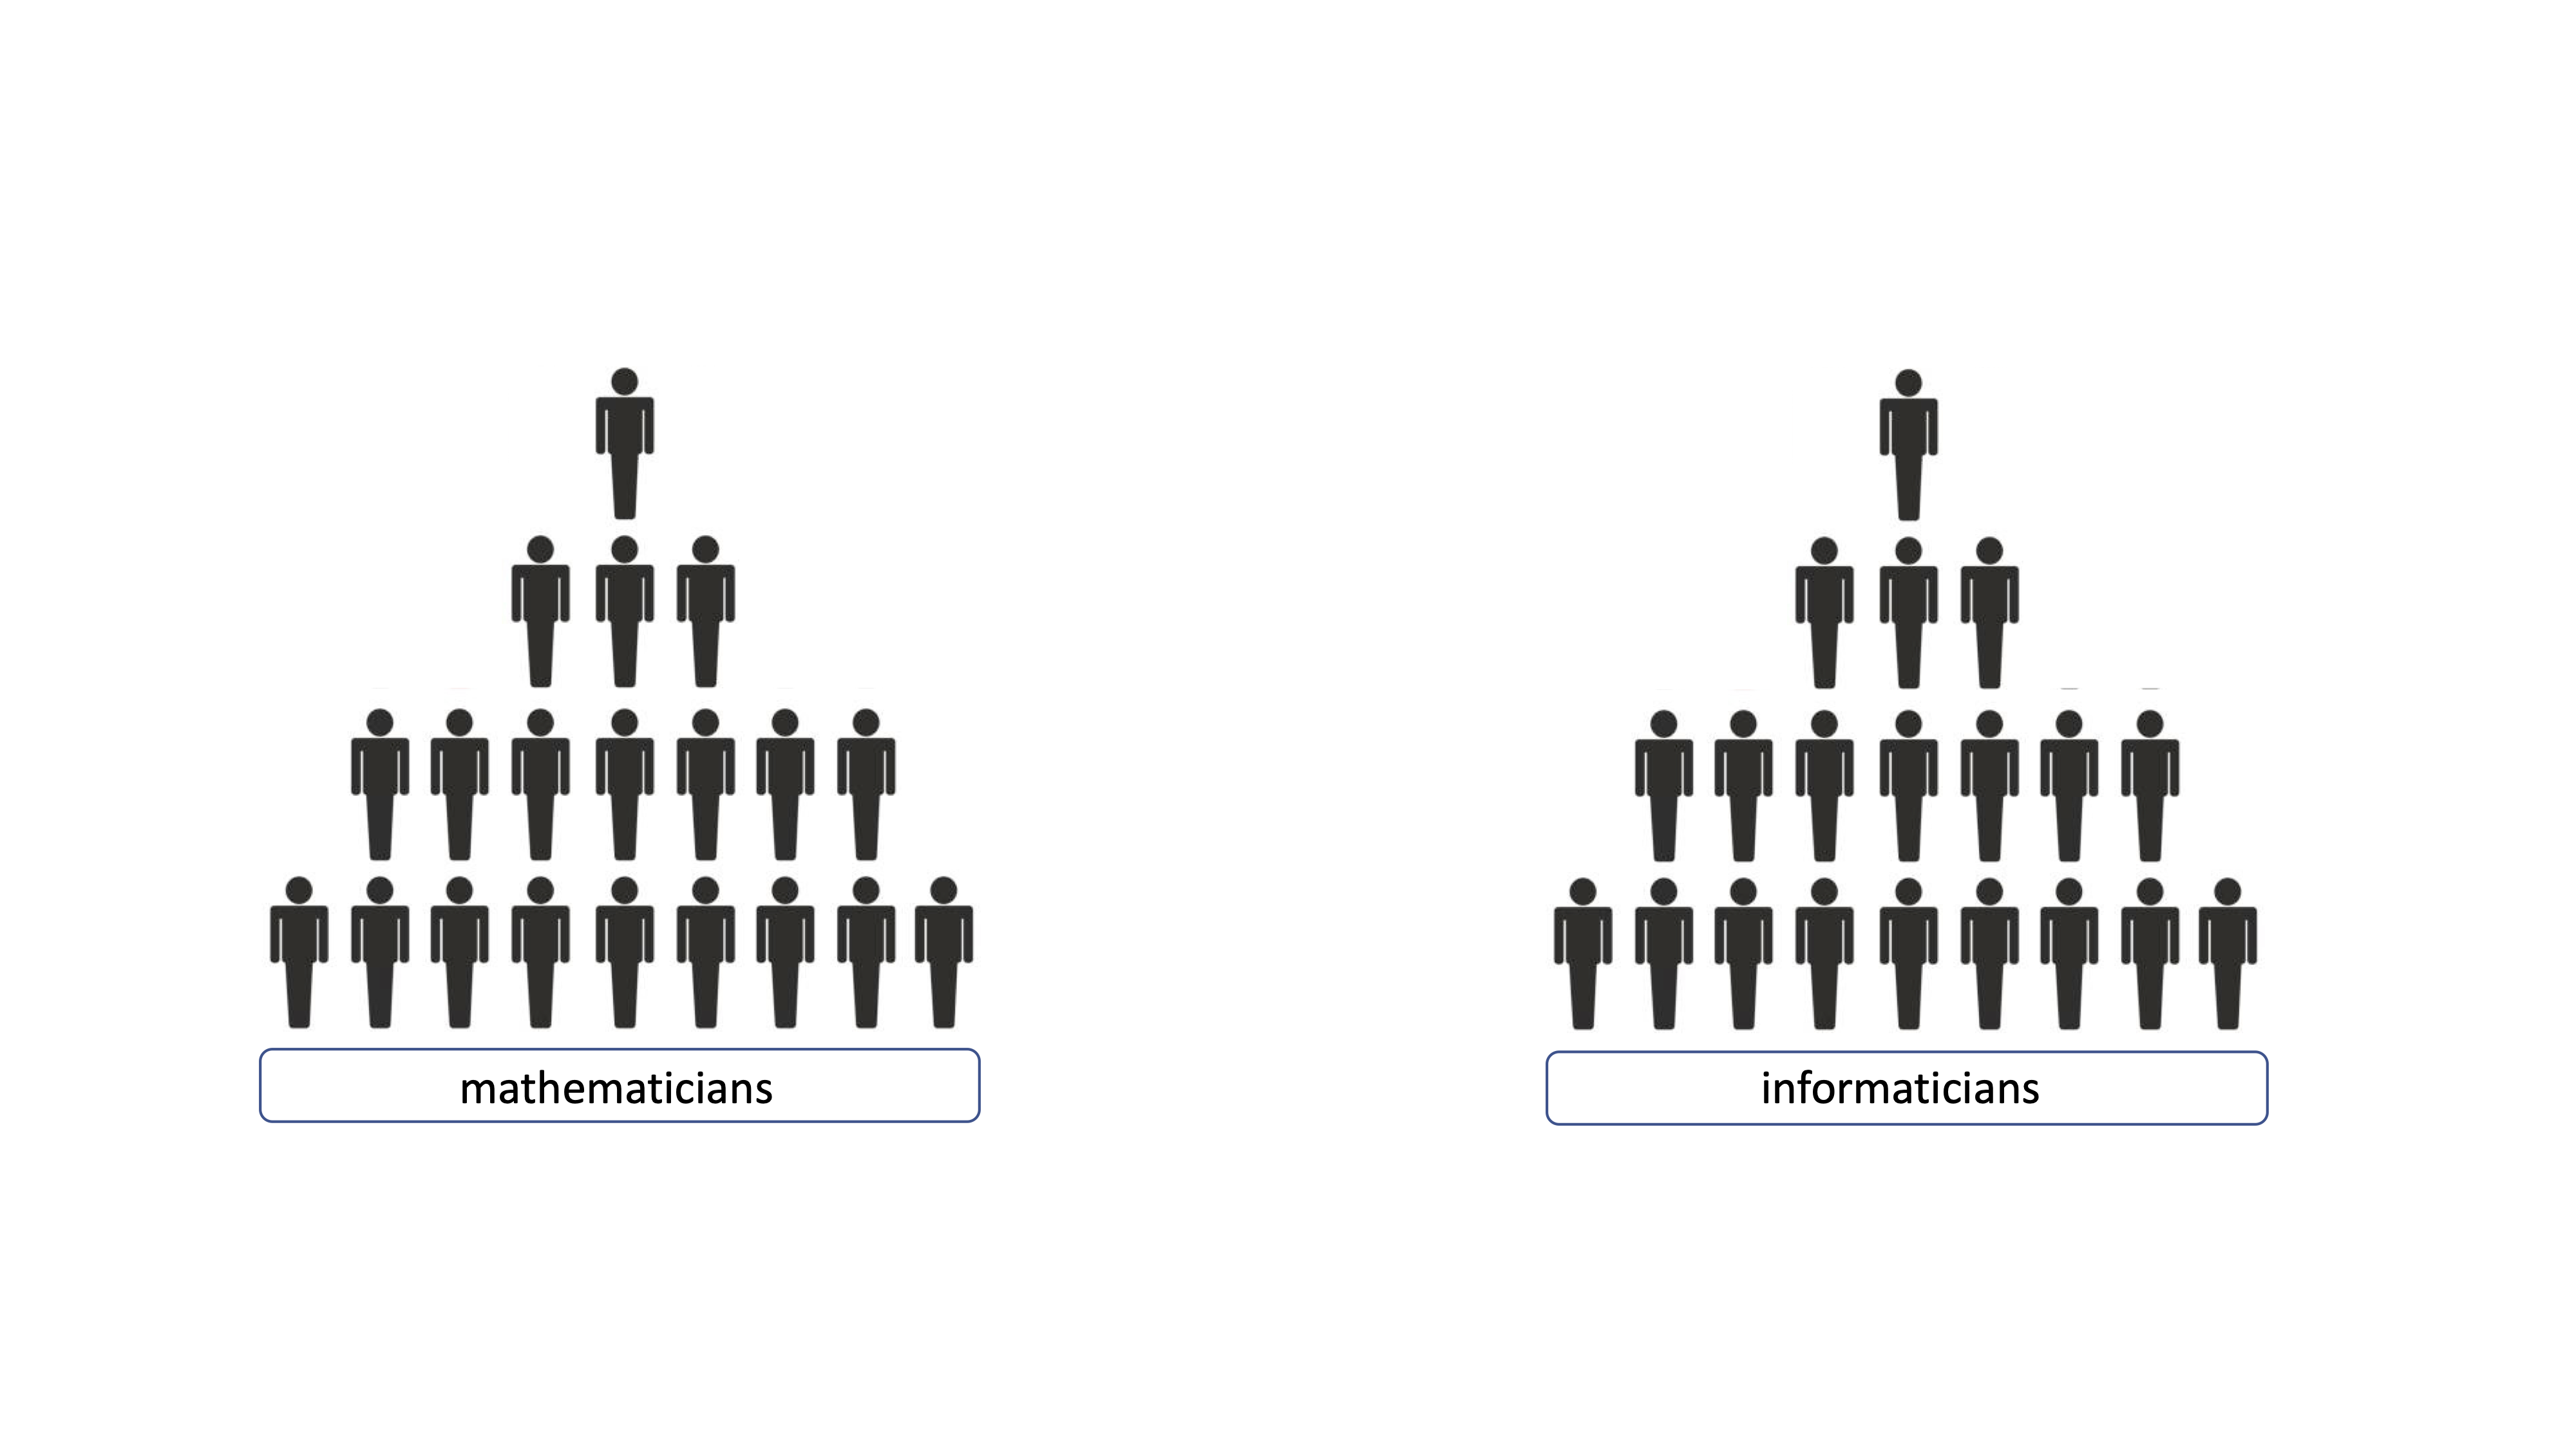
\includegraphics[width=12.5cm]{posJulia1.png}}
 }
  \only<2>{
  \textcolor{white}{A programming language for optimization}
 \hspace{-5mm}\centerline{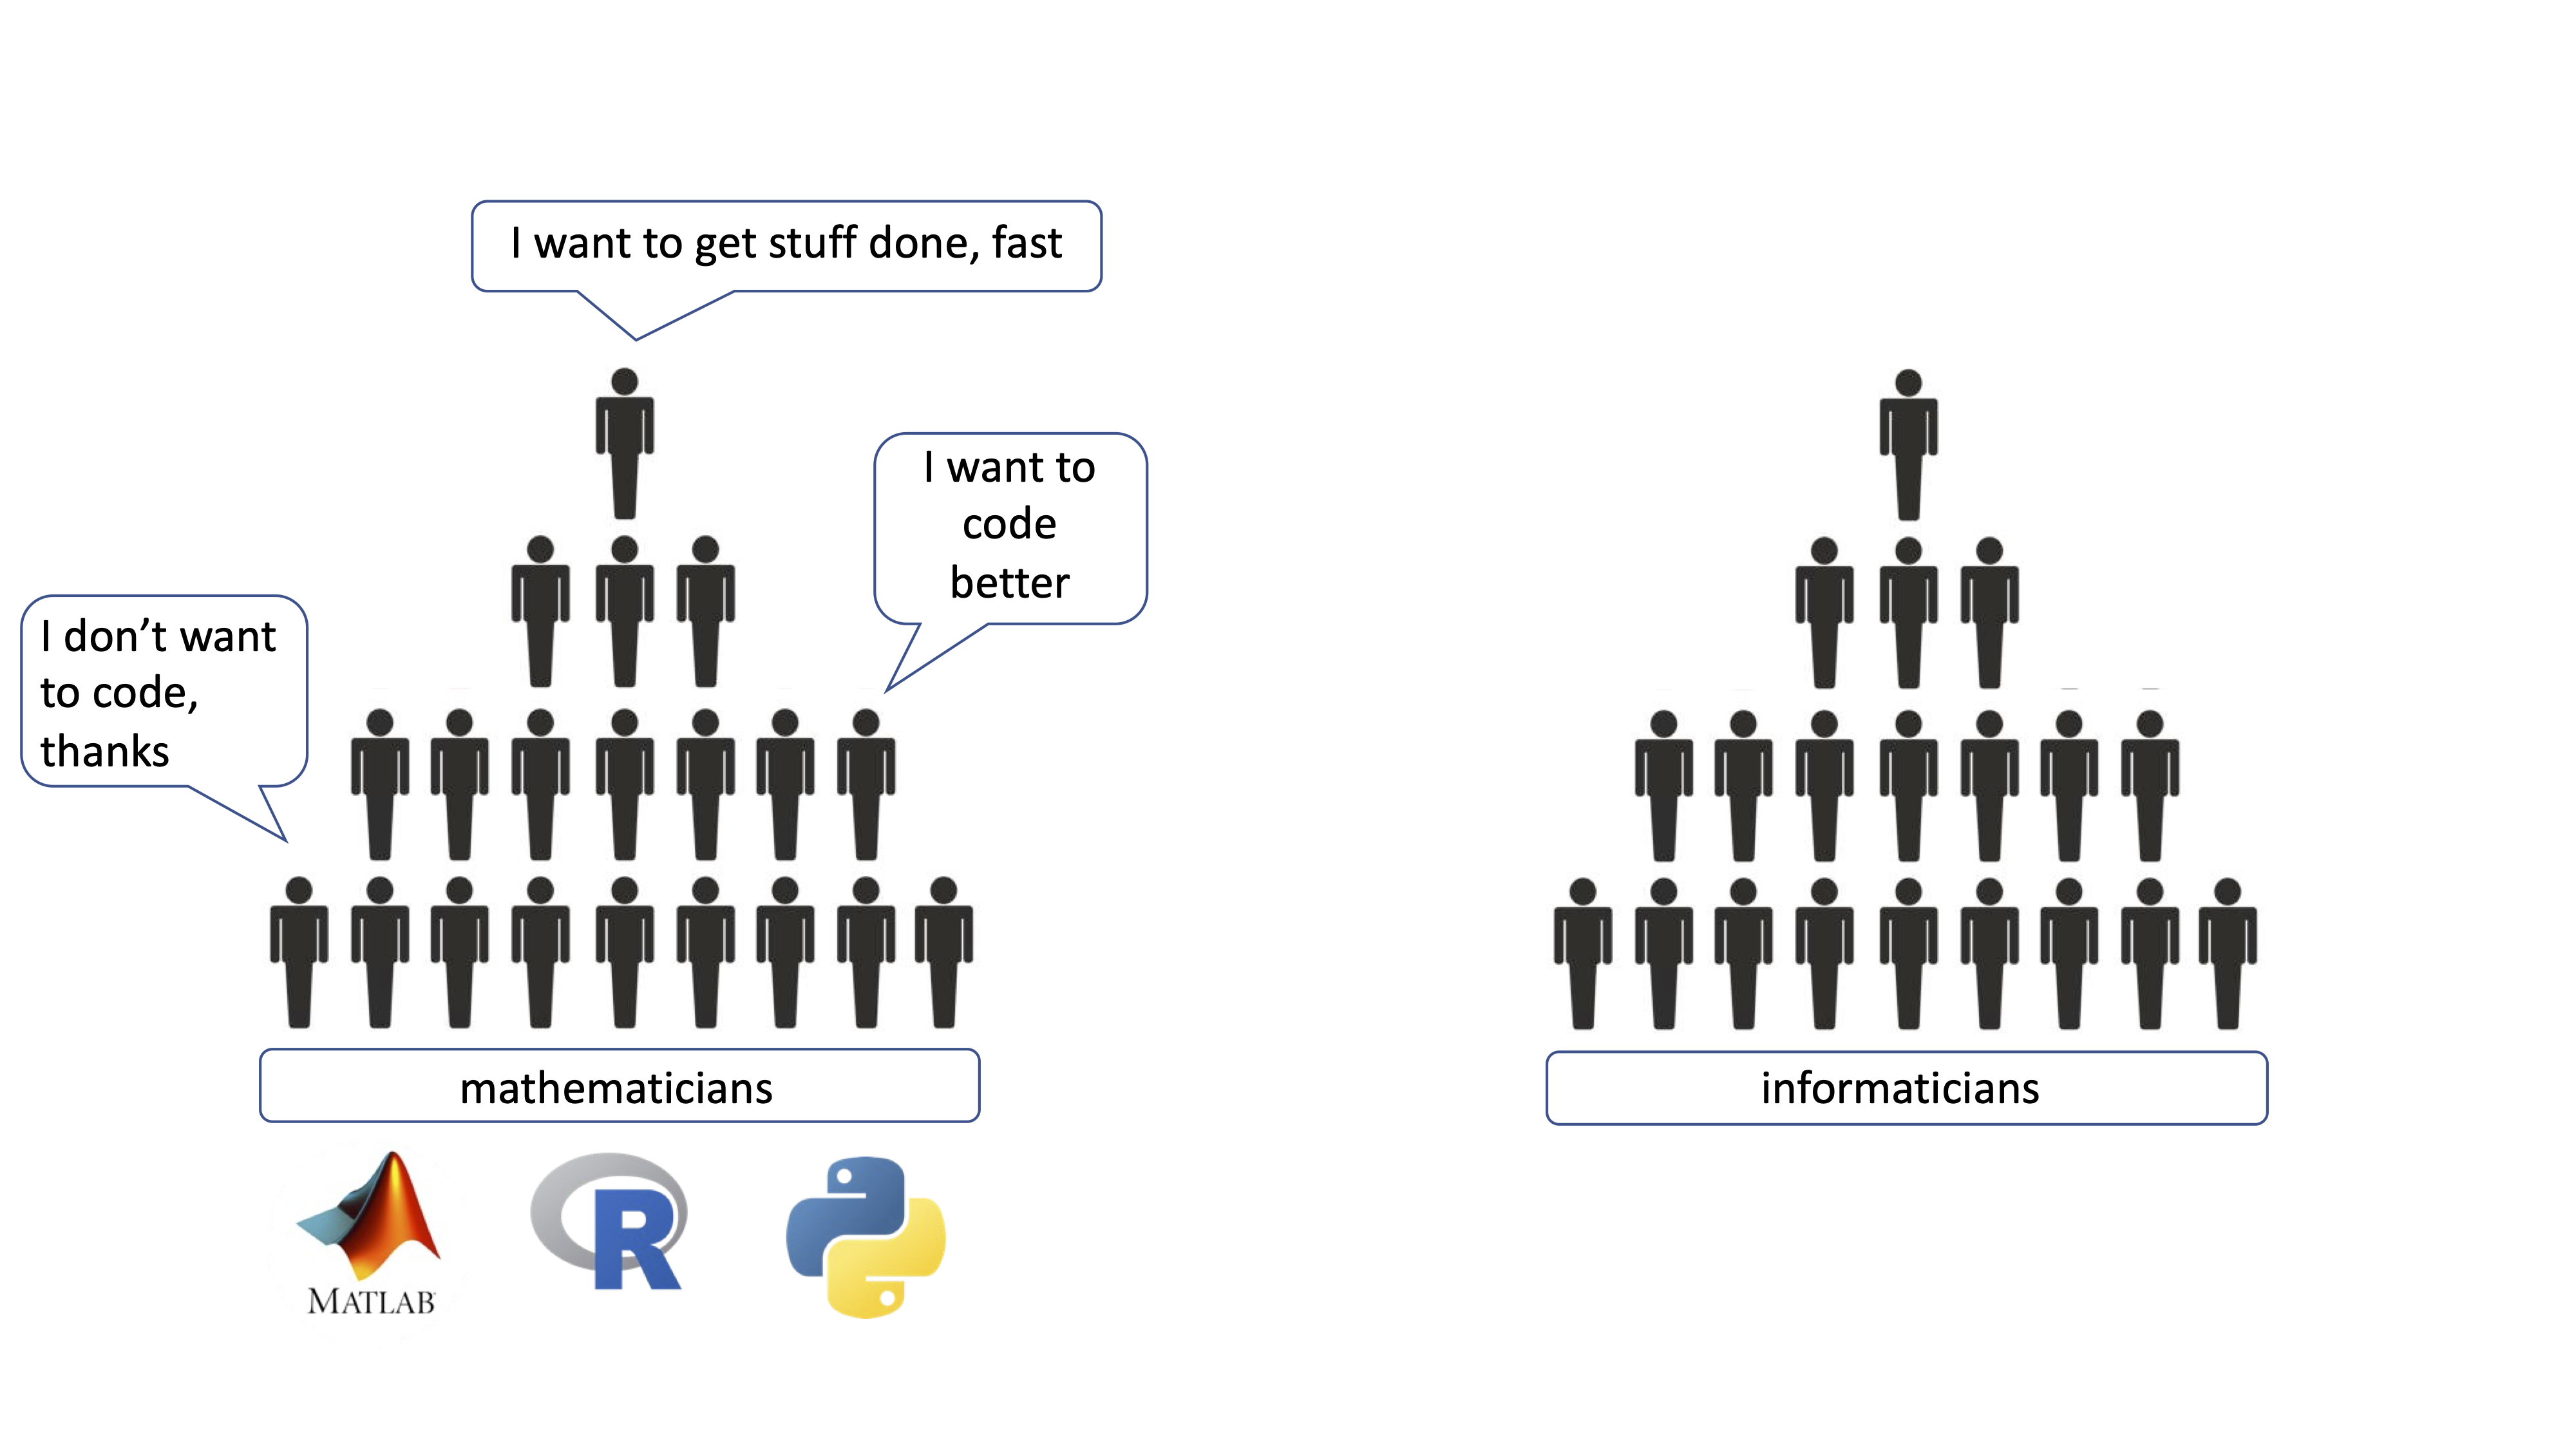
\includegraphics[width=12.5cm]{posJulia2.png}}
 }
  \only<3>{
  \textcolor{white}{A programming language for optimization}
 \hspace{-5mm}\centerline{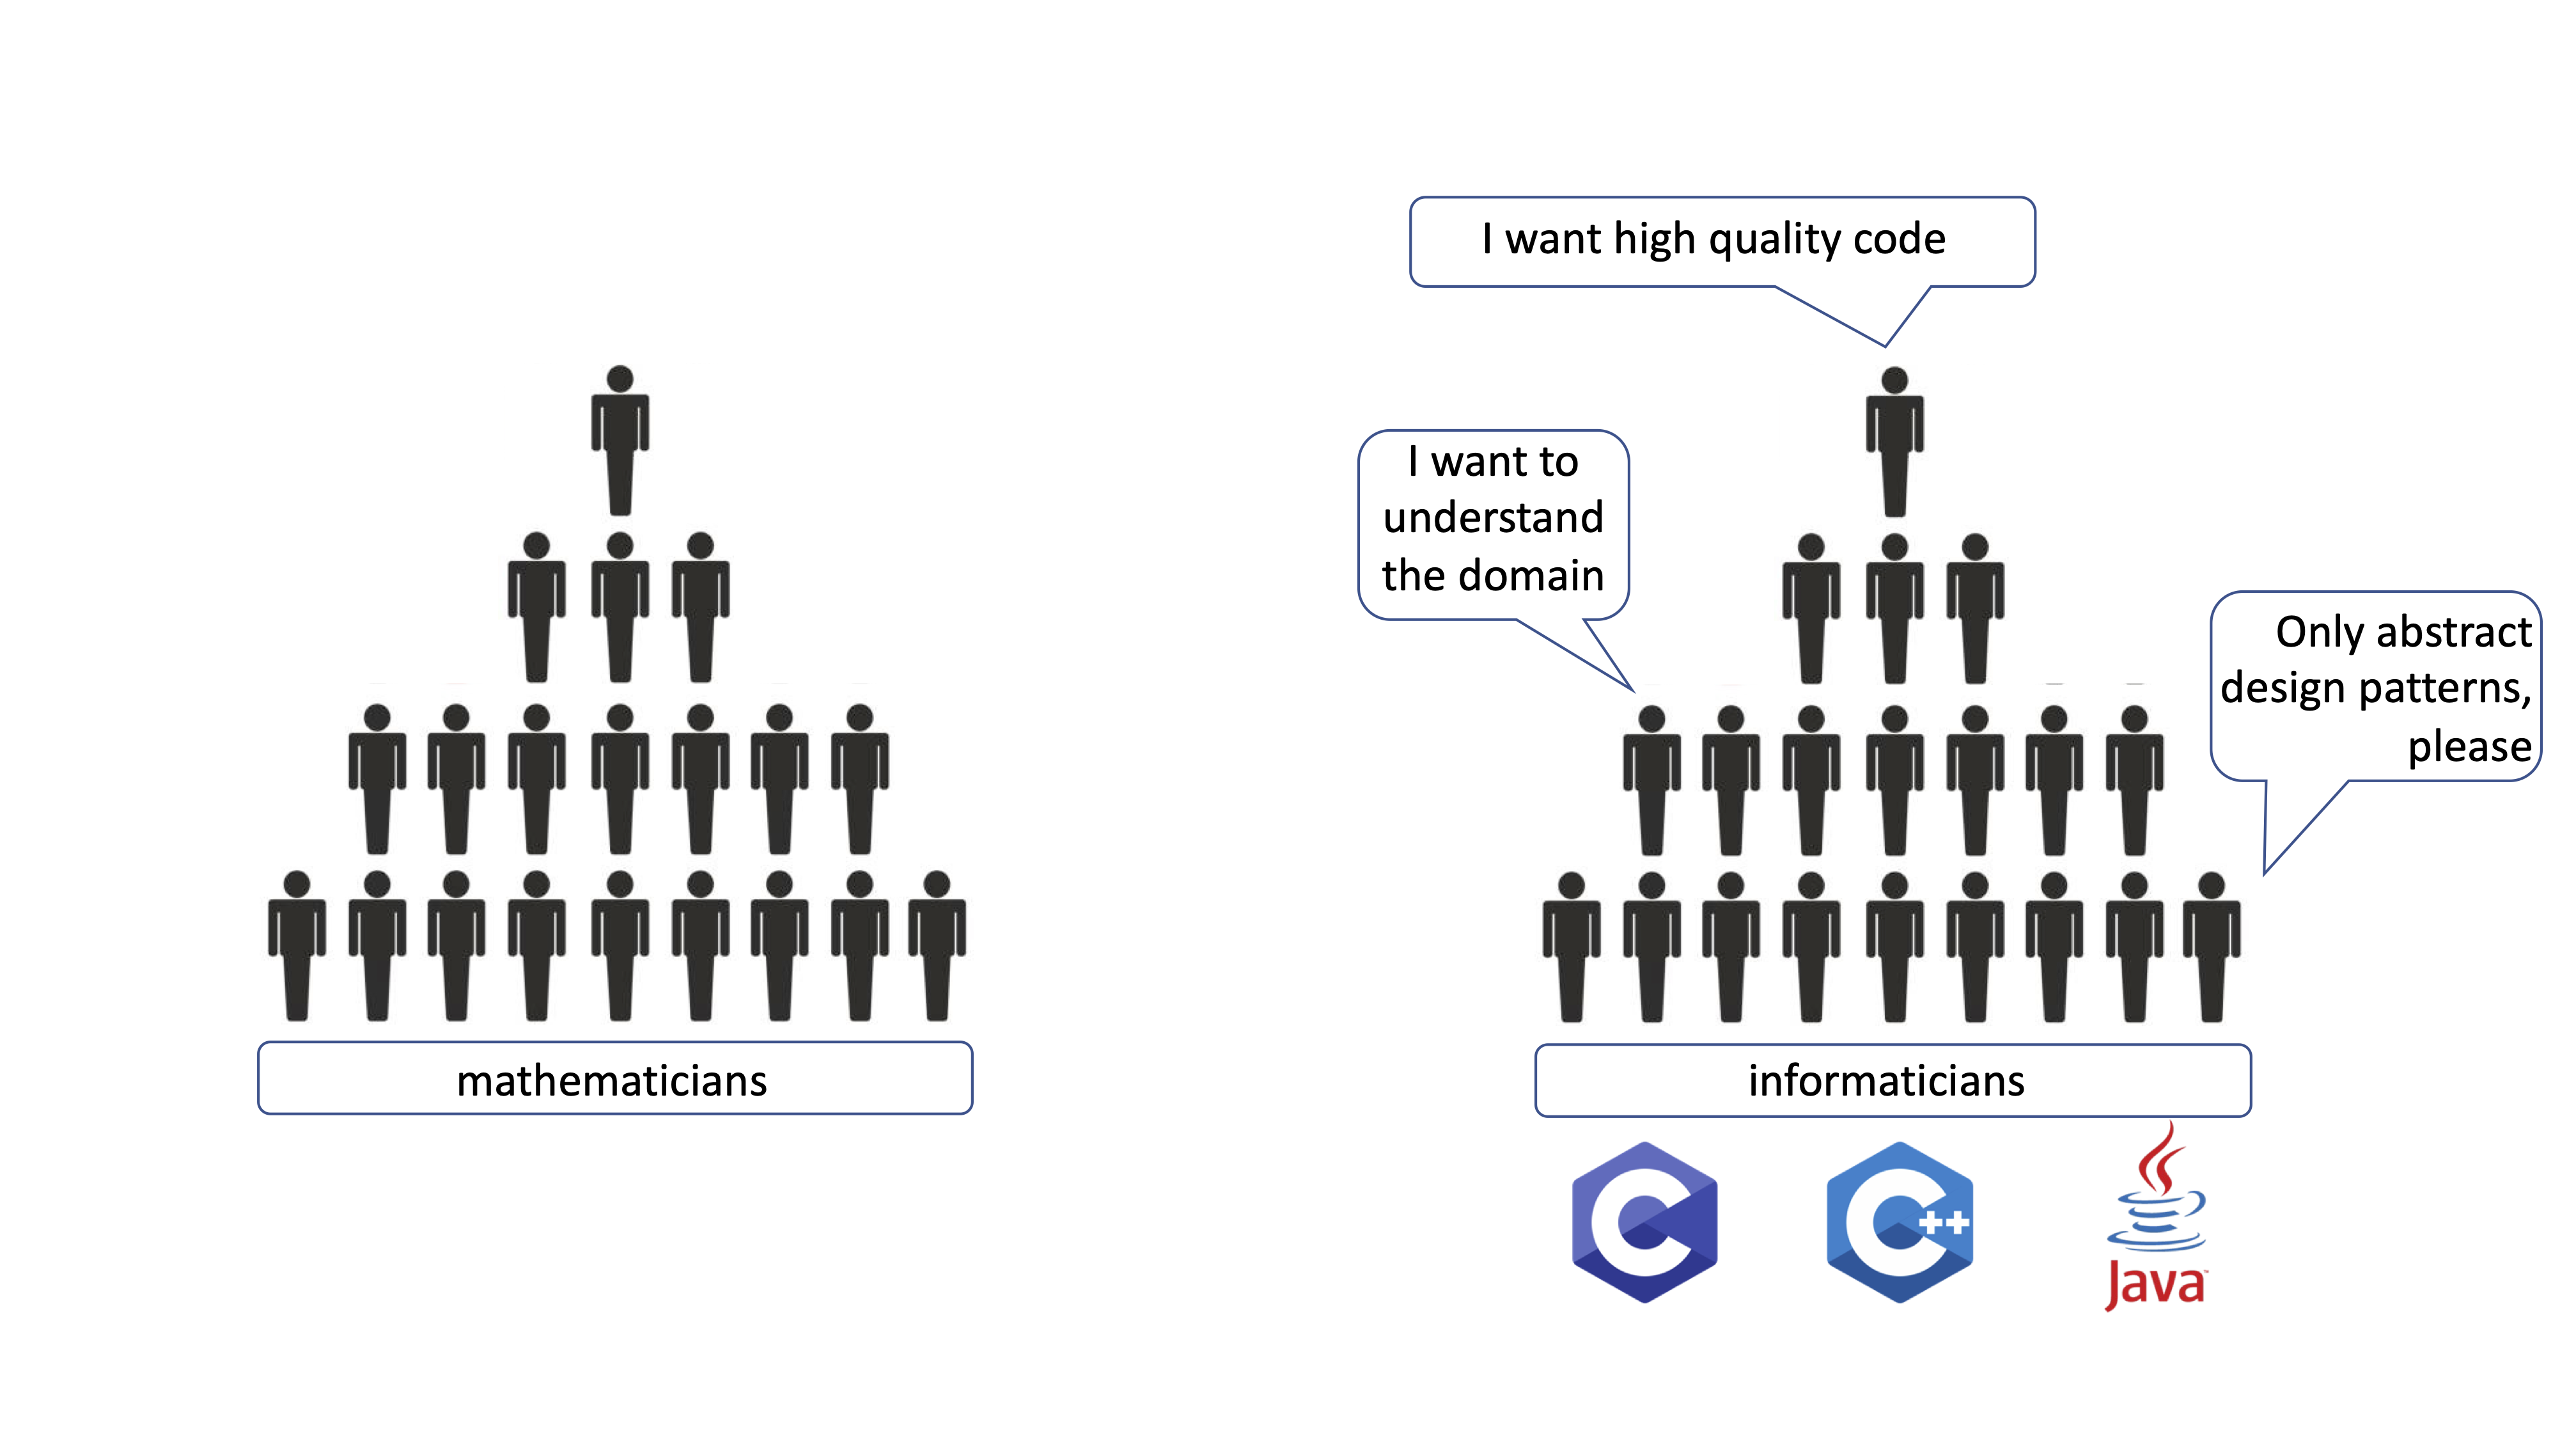
\includegraphics[width=12.5cm]{posJulia3.png}}
 }
  \only<4> {
  A programming language for optimization
 \hspace{-5mm}\centerline{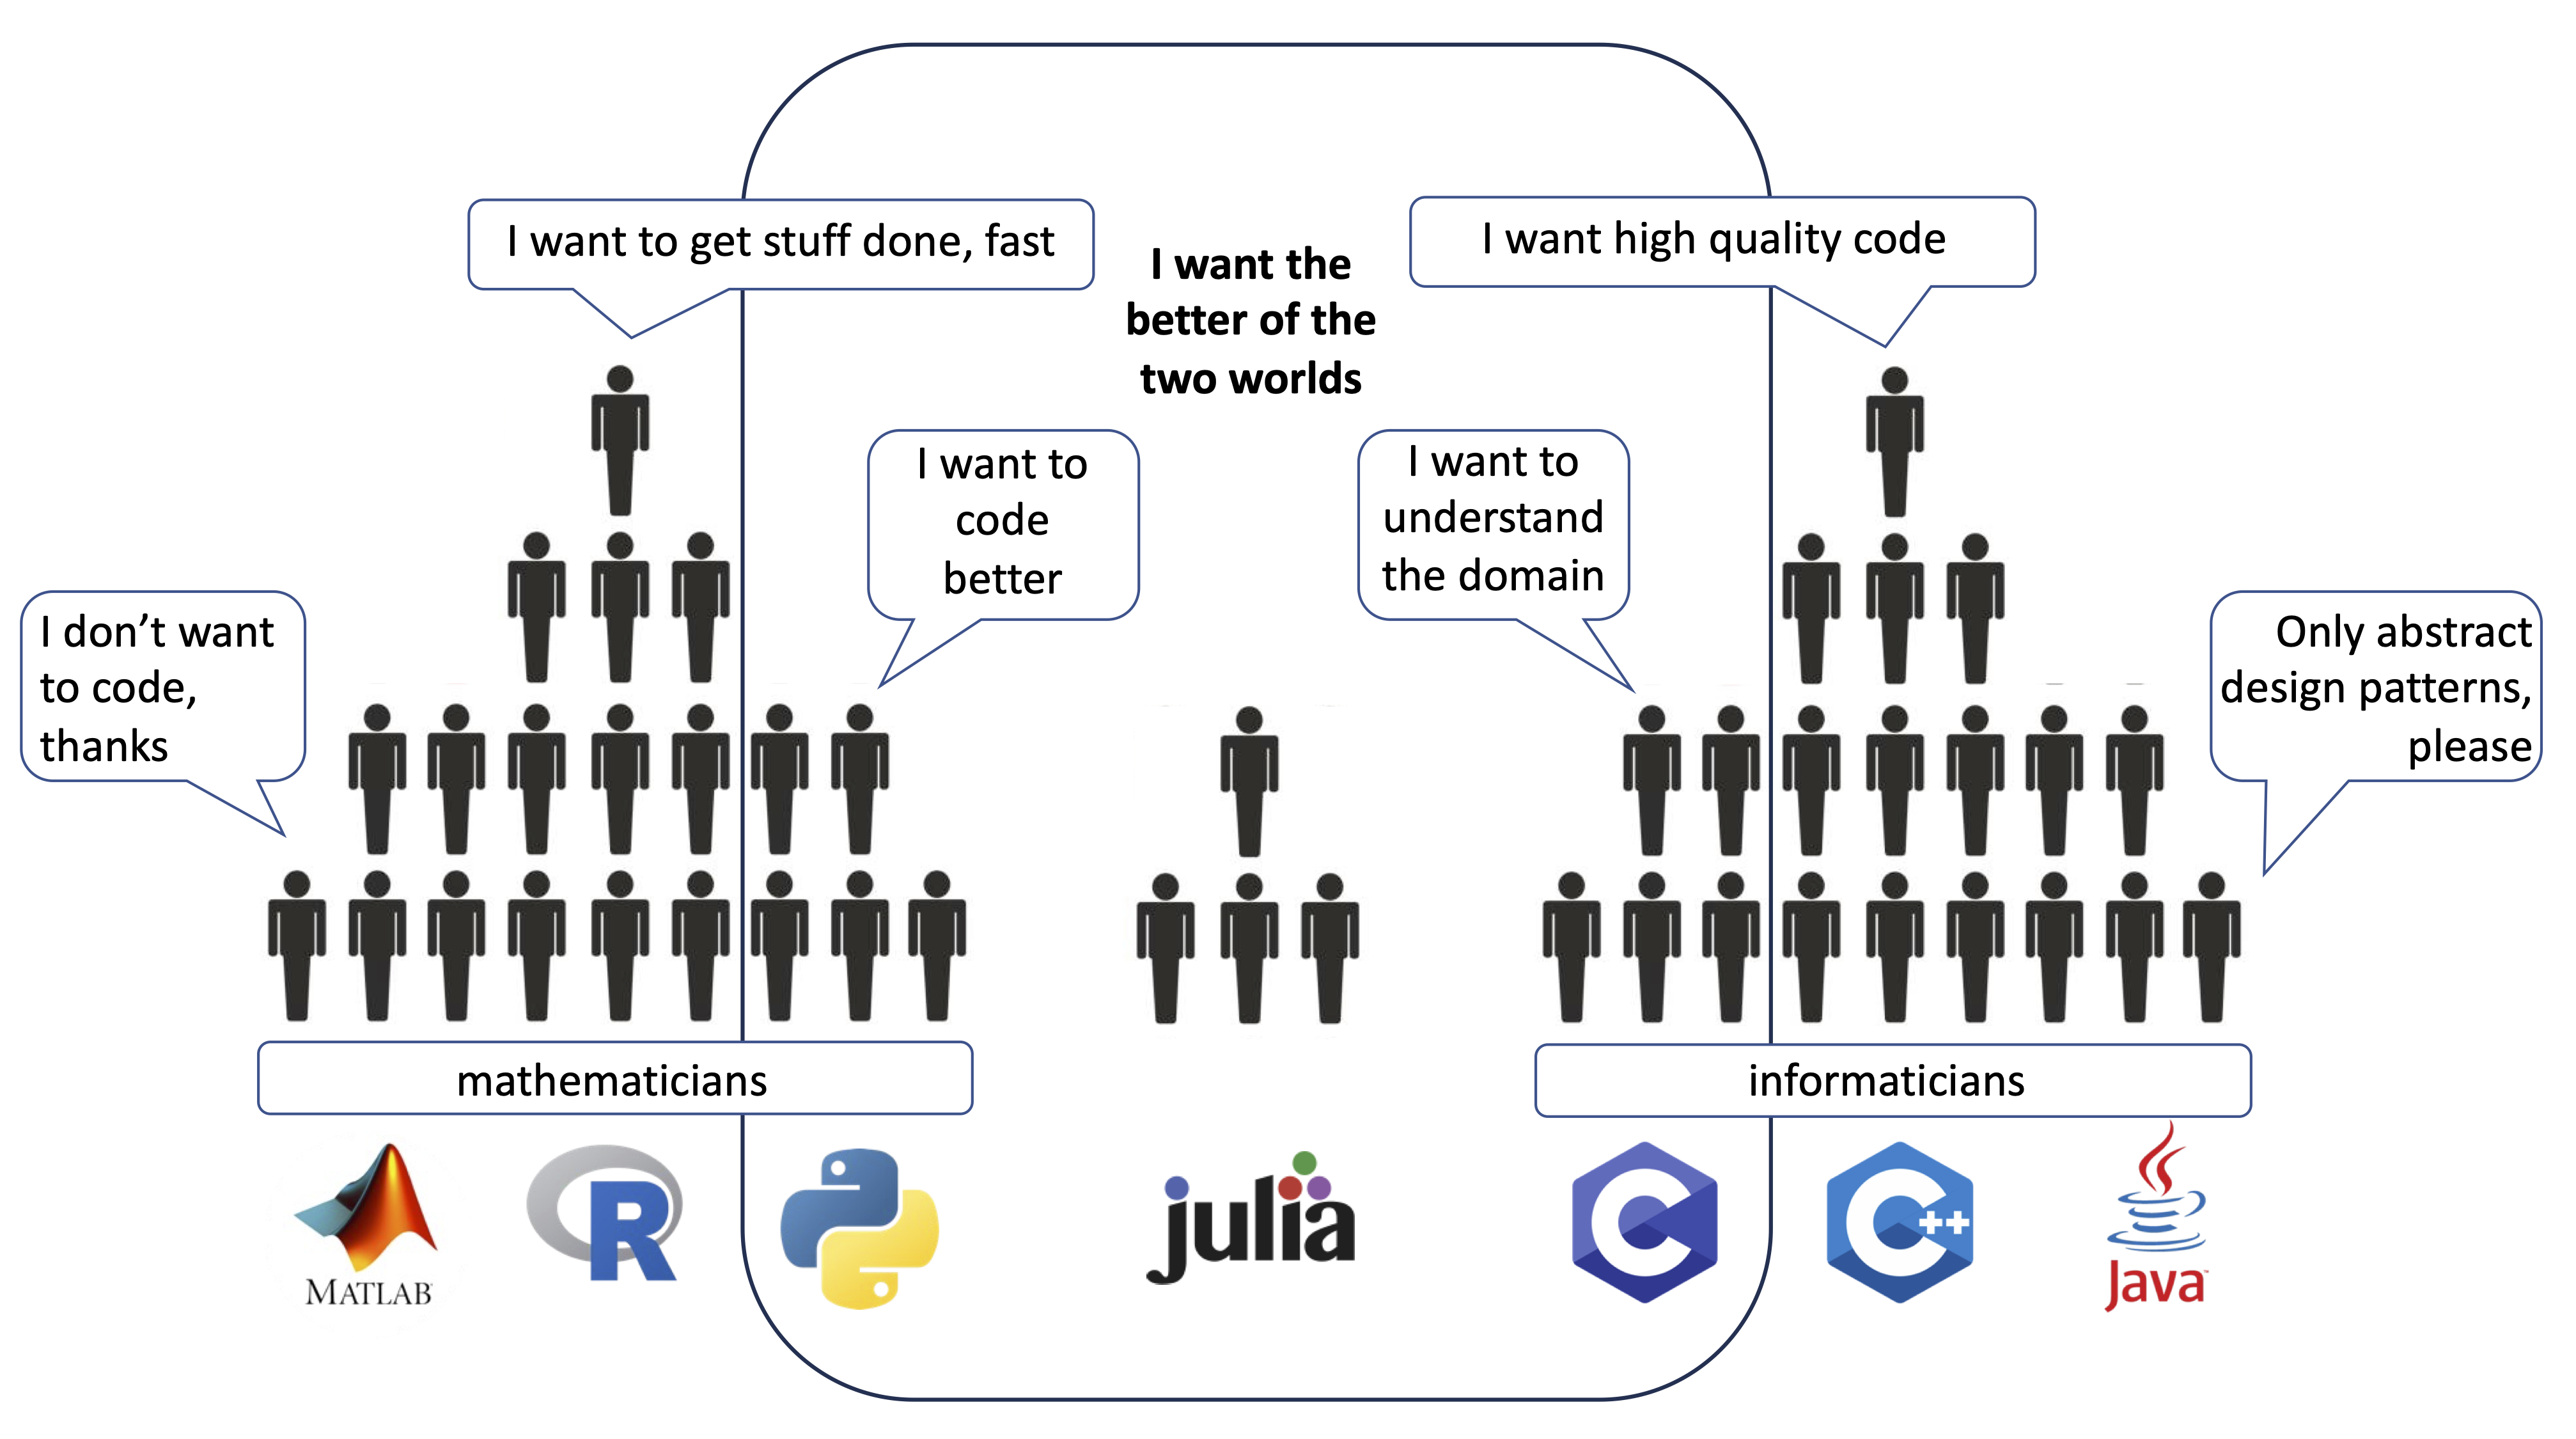
\includegraphics[width=12.5cm]{posJulia4.png}}
 }

\end{frame}

% 
% -------------------------------------------------------------------------------------------------------------------------------------------------------
%
\begin{frame}[fragile]
  \frametitle{Julia}
 \vspace{2mm}


  \only<1>{
   \textcolor{white}{LLVM: middleman between source code and compiled native code}
 \hspace{-5mm}
 \centerline{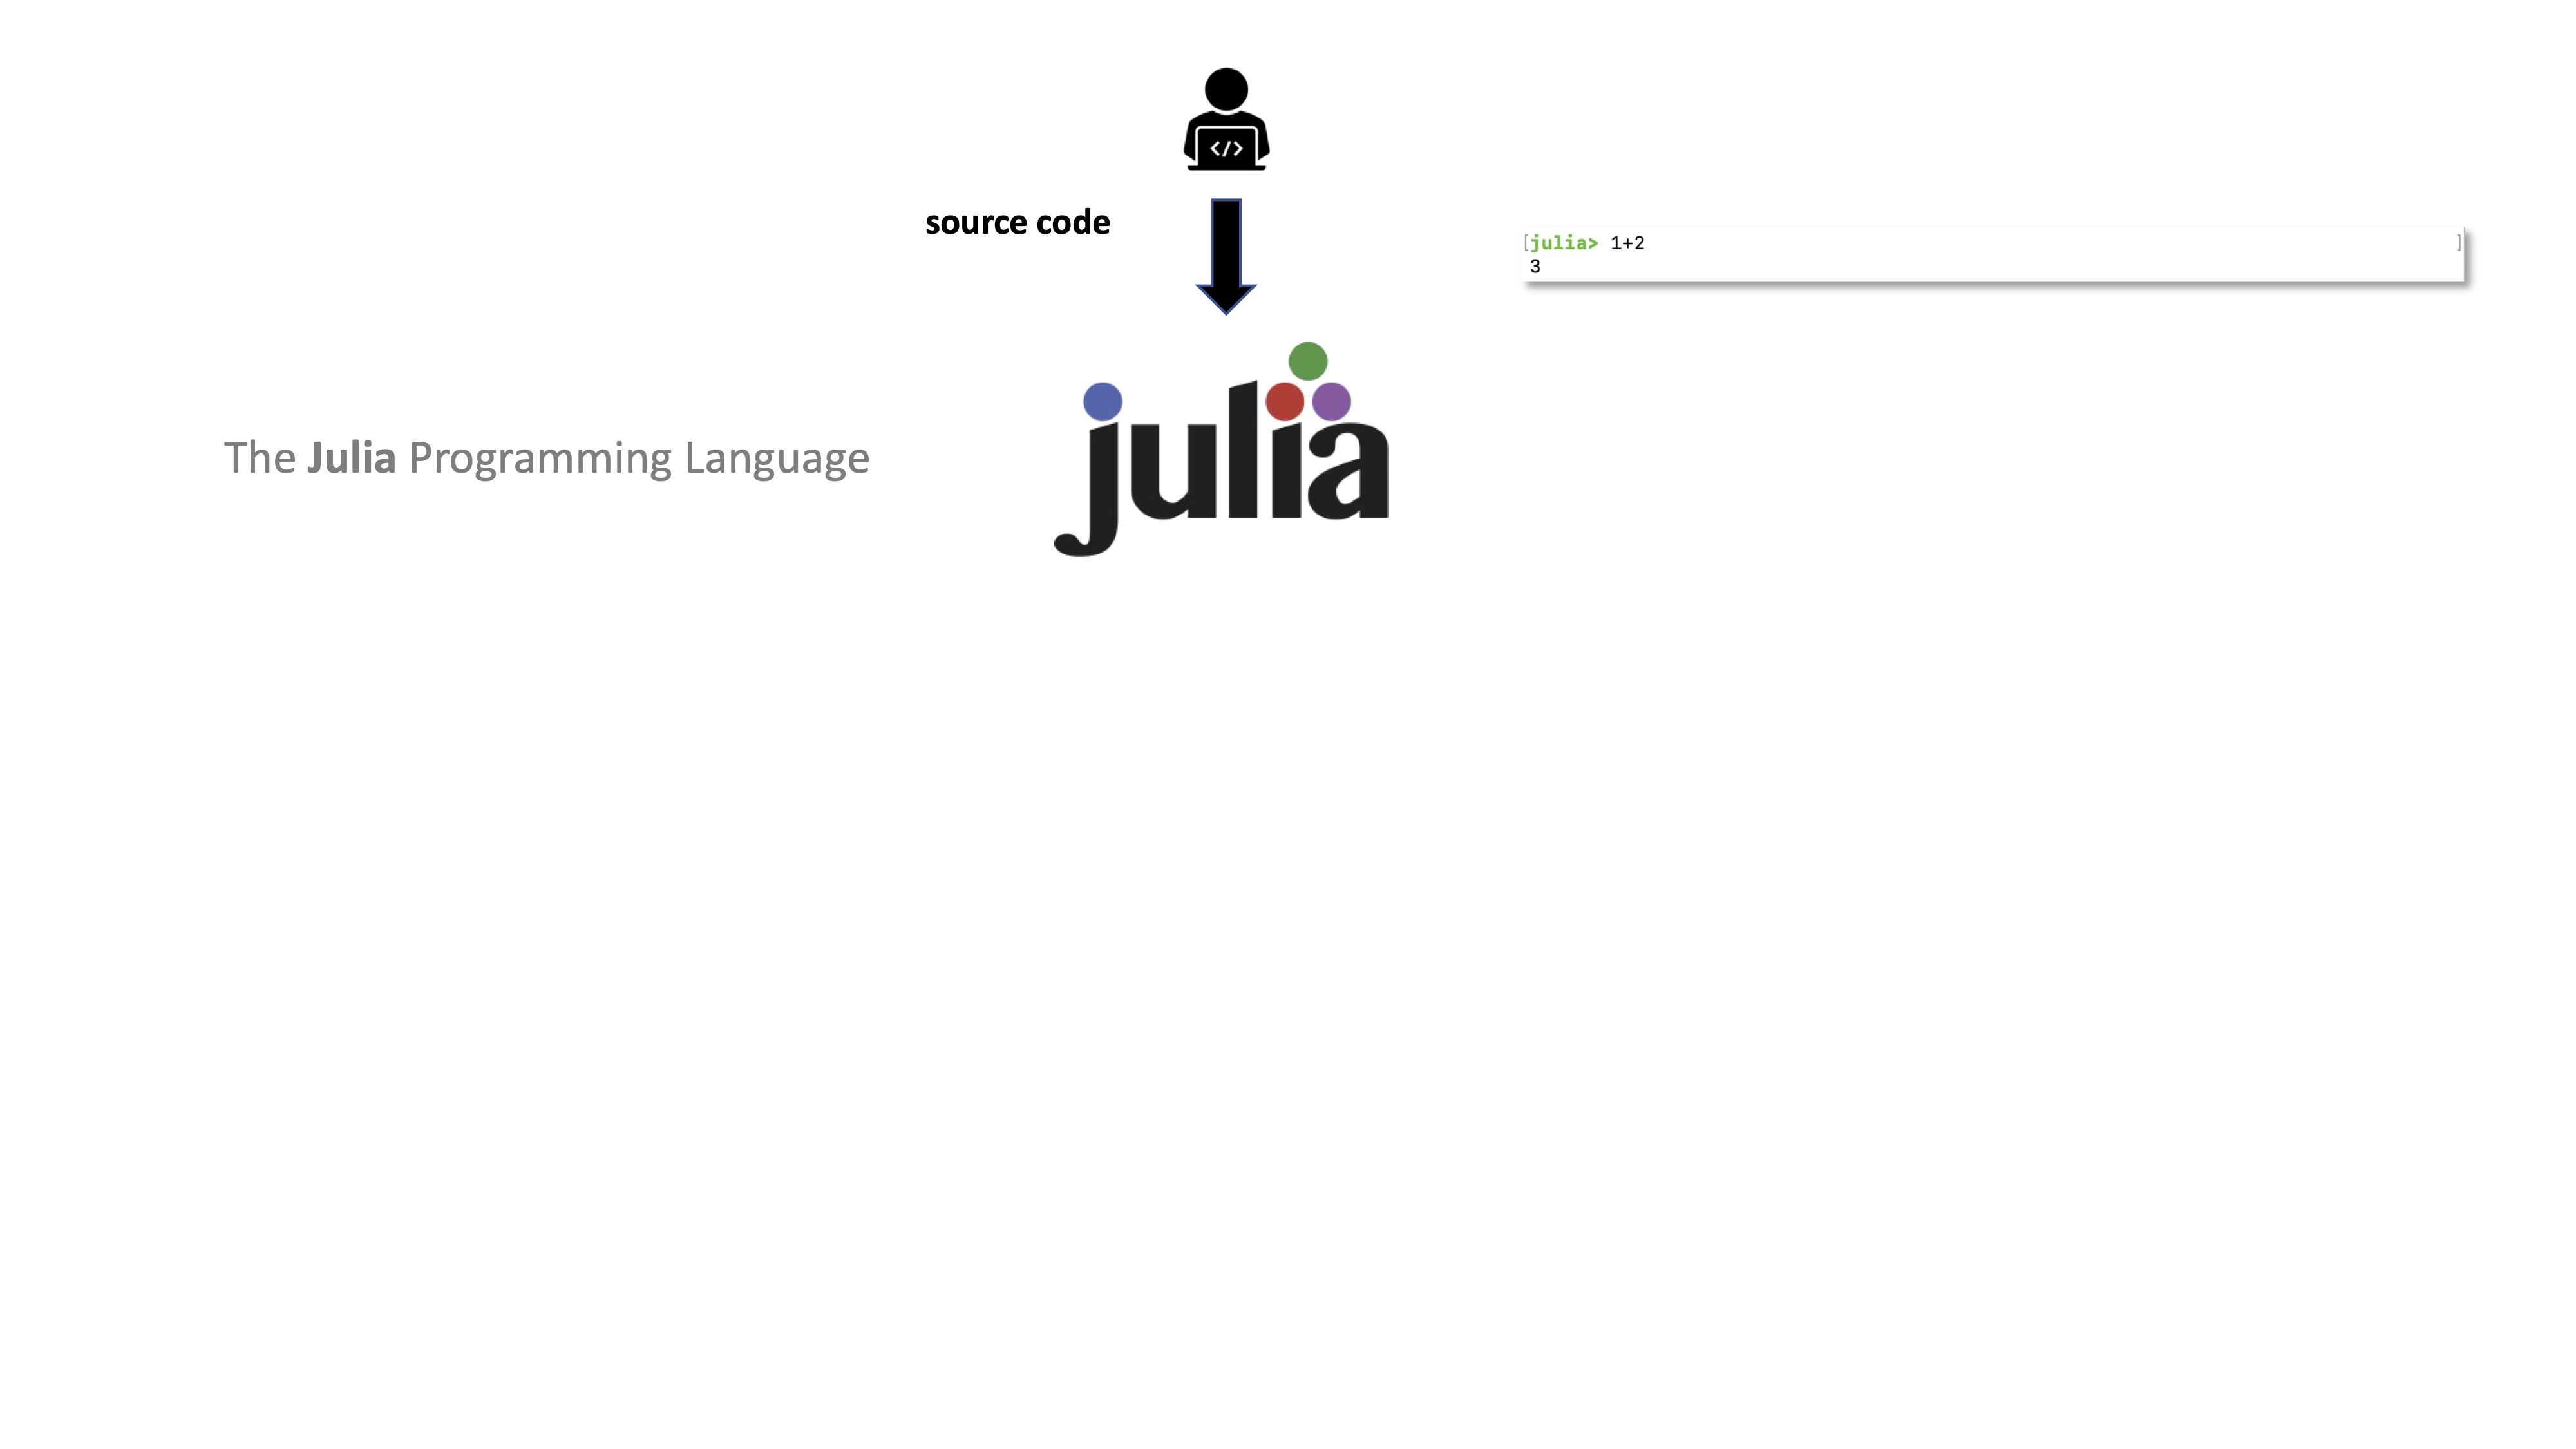
\includegraphics[width=12.5cm]{llvmJulia1.png}}
 }
  \only<2>{
  LLVM: middleman between source code and compiled native code
 \hspace{-5mm}
 \centerline{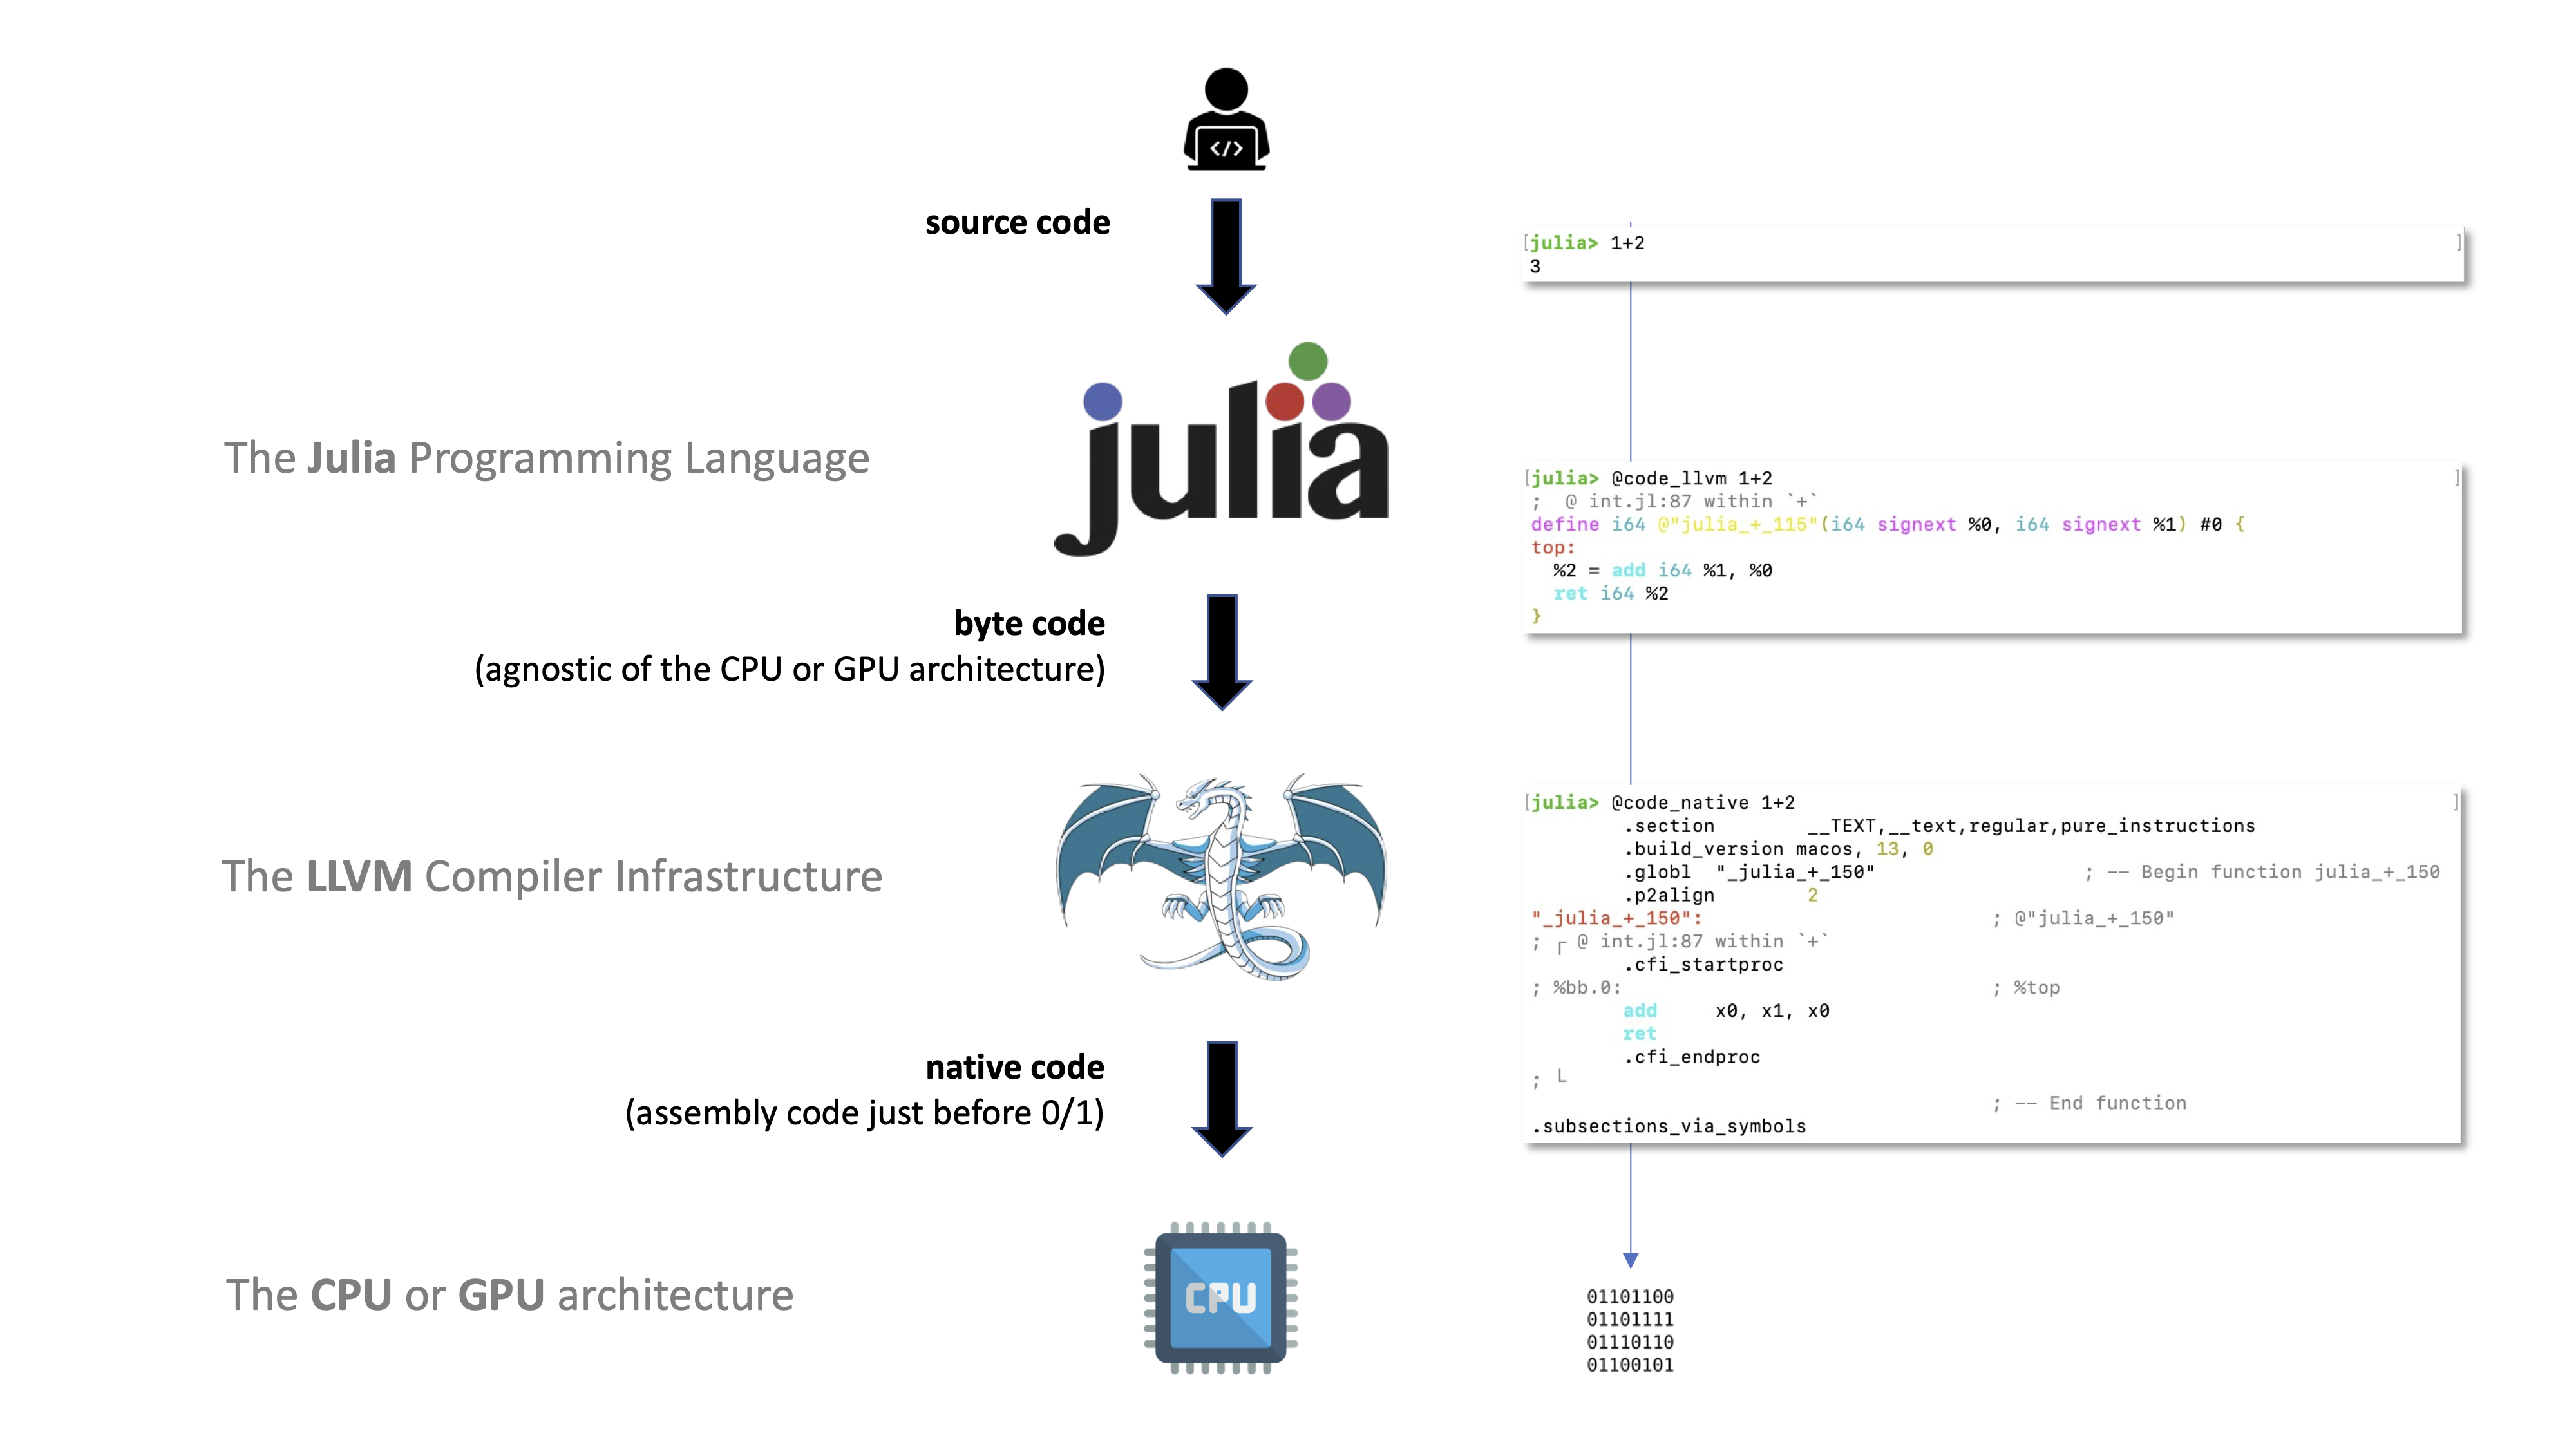
\includegraphics[width=12.5cm]{llvmJulia2.png}}
 }  
\end{frame}




% 
% -------------------------------------------------------------------------------------------------------------------------------------------------------
%

\begin{frame}
  \frametitle{Running a Julia code into...}
\vspace{3mm}

%    \begin{columns}
%          \begin{column}{0.5\textwidth}
%            ...the Julia REPL
%            \vspace{15mm}
%            
%            ...a notebook (jupyter)
%            \vspace{15mm}
%            
%              ....an IDE (VScode)
%                                    
%          \end{column}    
%          \begin{column}{0.5\textwidth}
%            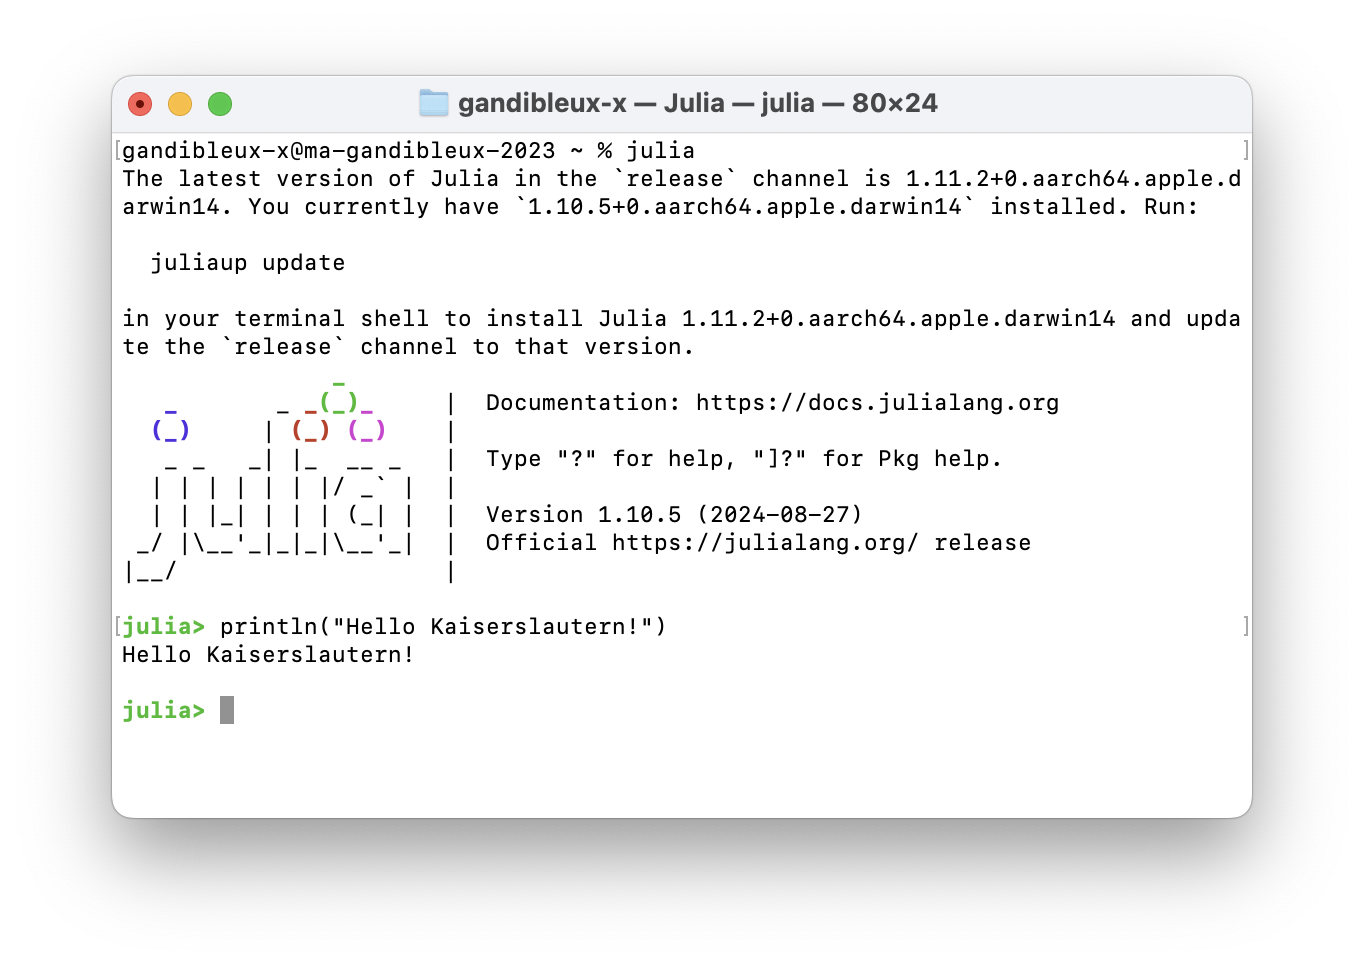
\includegraphics[angle=0,origin=c,height=35mm]{repl10.png} \vspace{-5mm}
%            
%            \hspace{5mm} 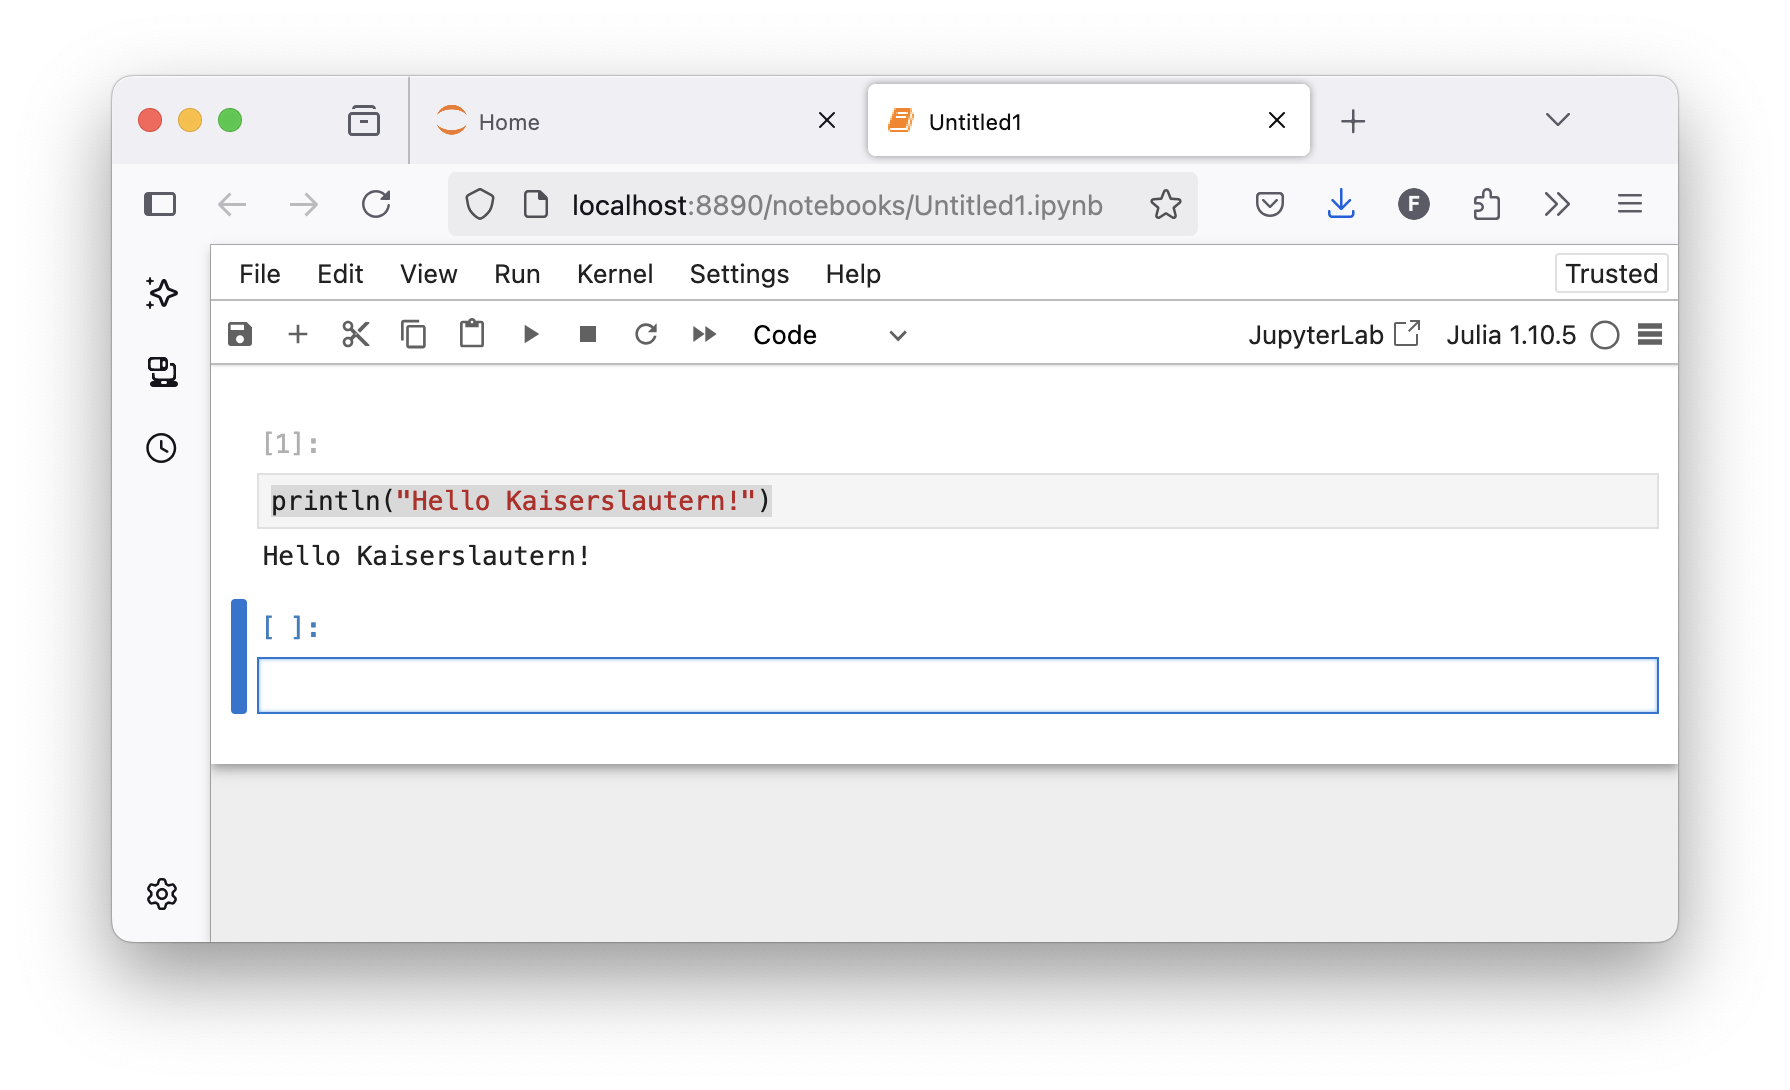
\includegraphics[angle=0,origin=c,height=35mm]{jupyter10.png} \vspace{-5mm}
%            
%            \hspace{10mm} 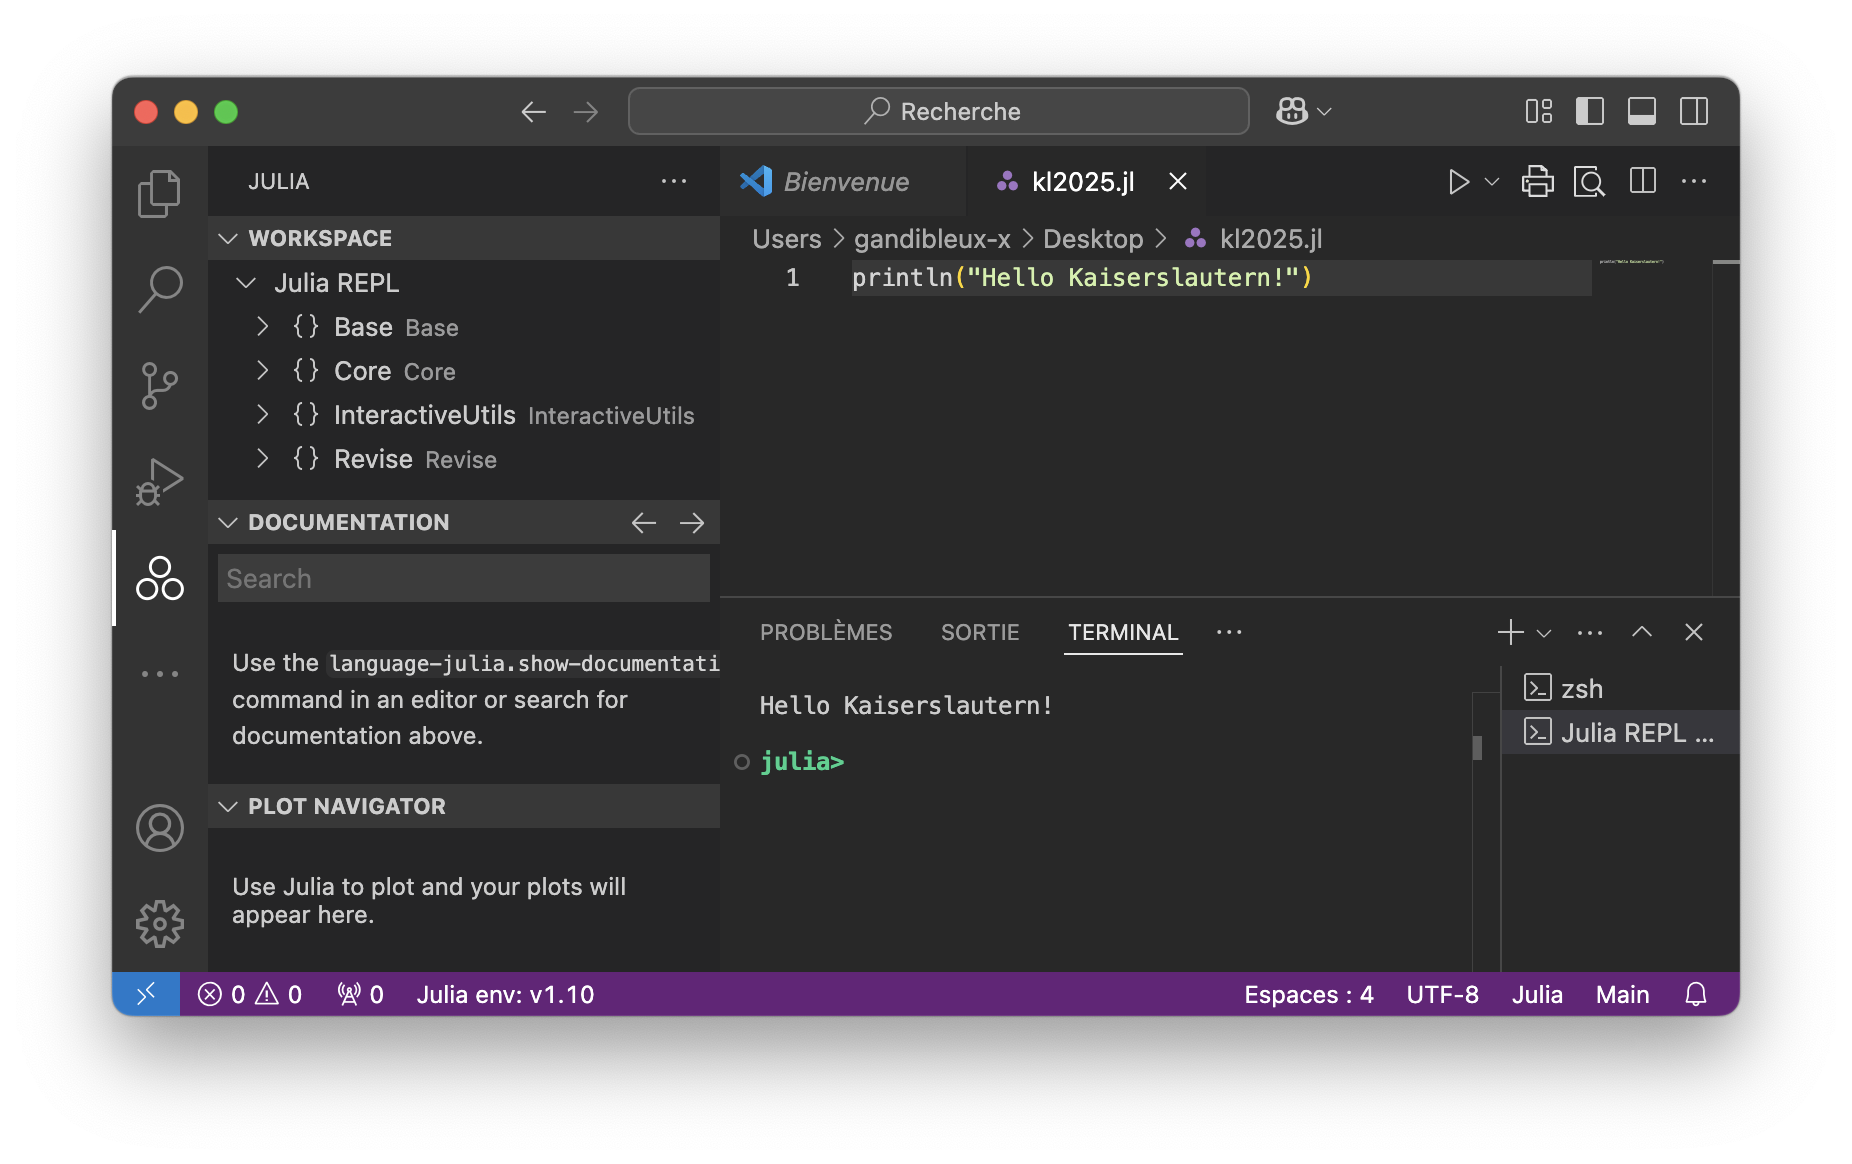
\includegraphics[angle=0,origin=c,height=35mm]{vscode10.png}                        
%          \end{column}      
%      \end{columns}
         
      
    \begin{columns}
      \begin{column}{0.3\textwidth}
      \vspace{0mm}
      ...the Julia REPL
      
       \centerline{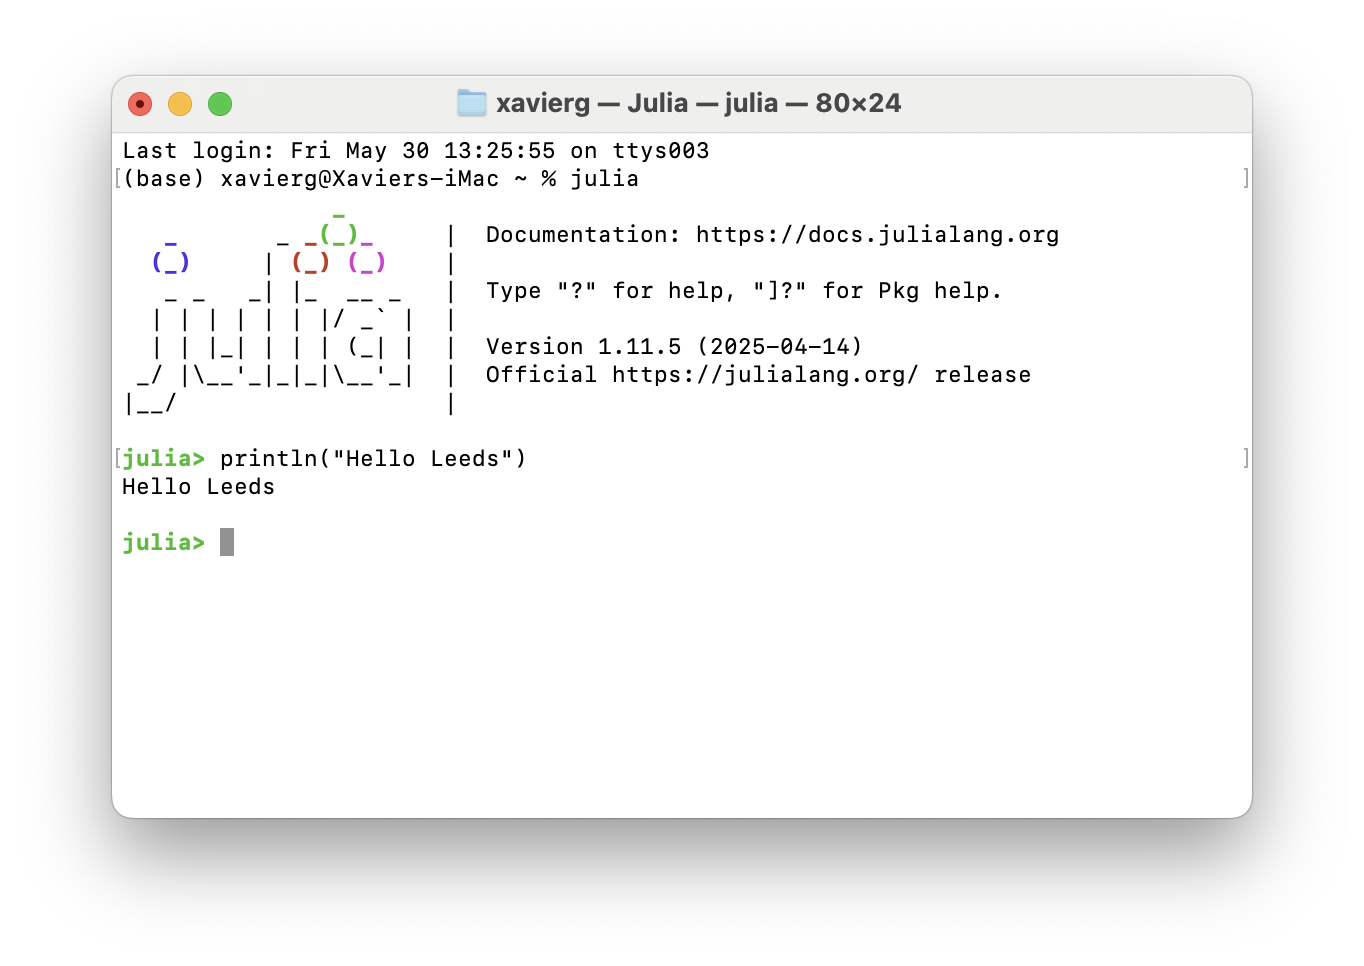
\includegraphics[angle=0,origin=c,height=35mm]{replLeeds.png}}      
       
       \vspace{15mm}
      \end{column}
      
      \begin{column}{0.33\textwidth}
      \vspace{5mm}
      
      ...a notebook \\ (e.g. jupyter)
      
      \centerline{{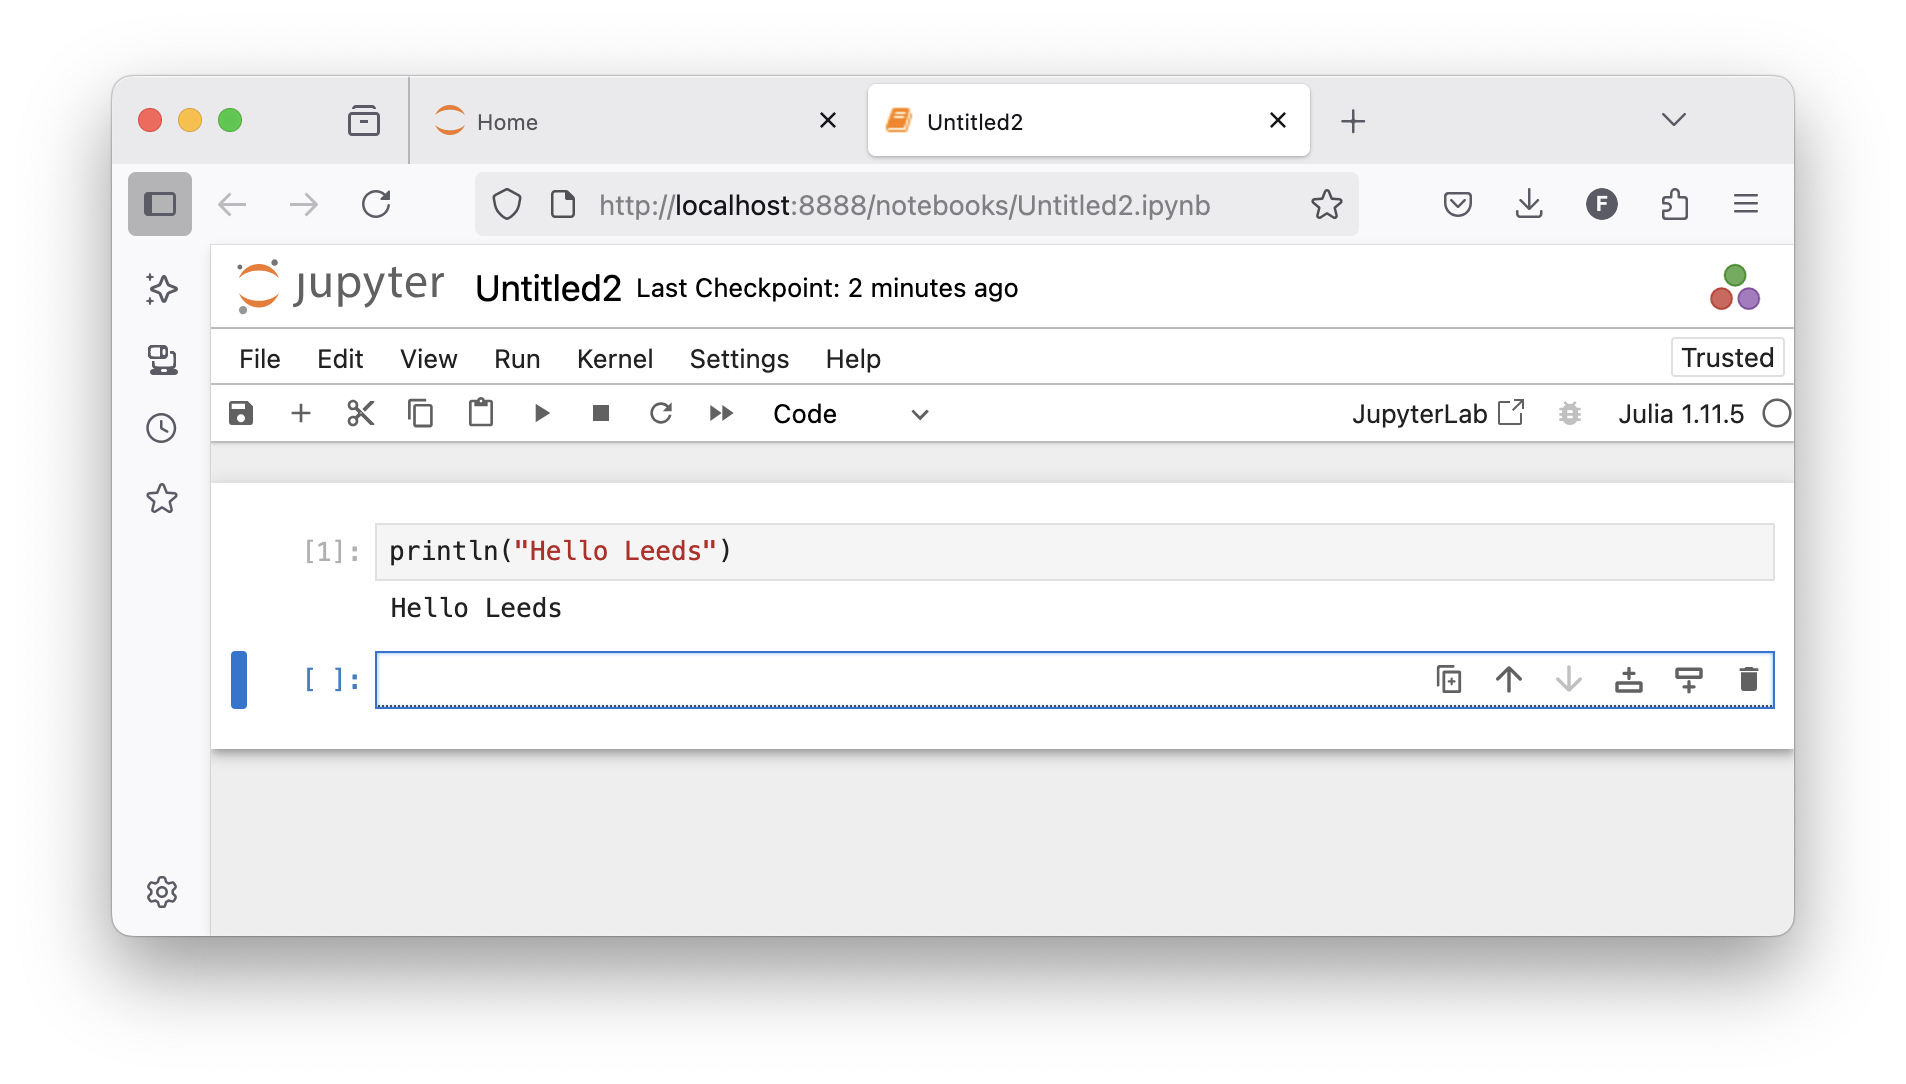
\includegraphics[angle=0,origin=c,height=30mm]{jupyterLeeds.png}}}      
      
      \vspace{10mm}
      \end{column}
      
      \begin{column}{0.3\textwidth}
      \vspace{10mm}
      
      ...an IDE \\ (e.g. VScode)
      
      \centerline{
\includegraphics[angle=0,origin=c,height=30mm]{vscodeLeeds.png}}      
      \vspace{5mm}            
      \end{column}  
          
      \end{columns}
      \vspace{5mm}
\hfill  ... or also in command line into a terminal.

\end{frame}



% 
% -------------------------------------------------------------------------------------------------------------------------------------------------------
%

\begin{frame}
  \frametitle{Example (1/2)}
\vspace{3mm}
   
          \begin{columns}
      \begin{column}{0.33\textwidth}

\centerline{MATLAB}
\medskip
{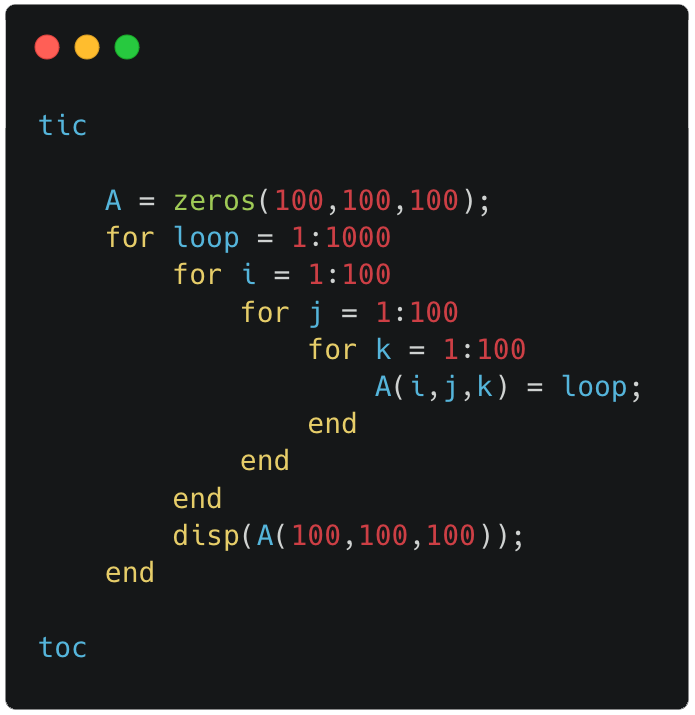
\includegraphics[angle=0,origin=t,width=39.6mm]{exempleMatLab.png}} 
\vspace{1.5mm}

      \end{column}
      
      \begin{column}{0.32\textwidth}

\centerline{Julia} 
\medskip
{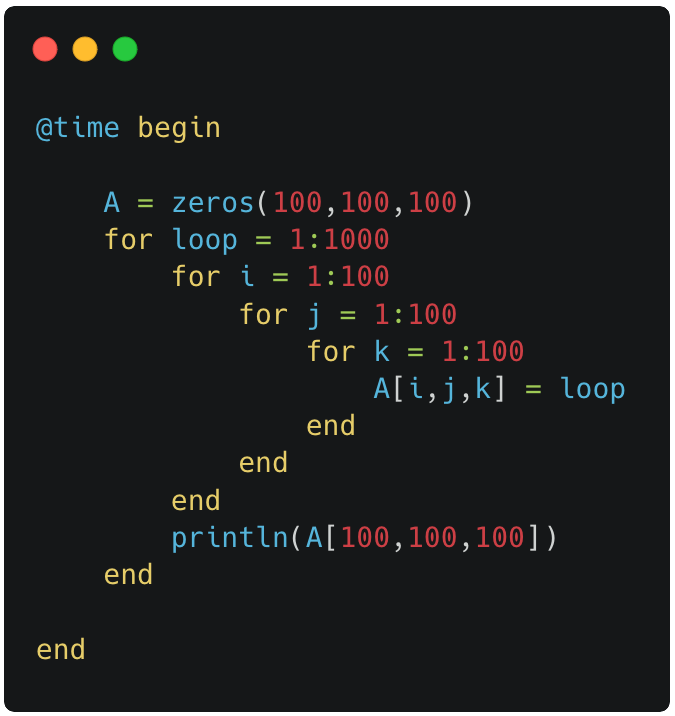
\includegraphics[angle=0,origin=t,width=38.5mm]{exempleJL.png}}
\vspace{1.5mm}       
 
      \end{column}  


      \begin{column}{0.32\textwidth}

\centerline{C} 
\vspace{1.7mm}
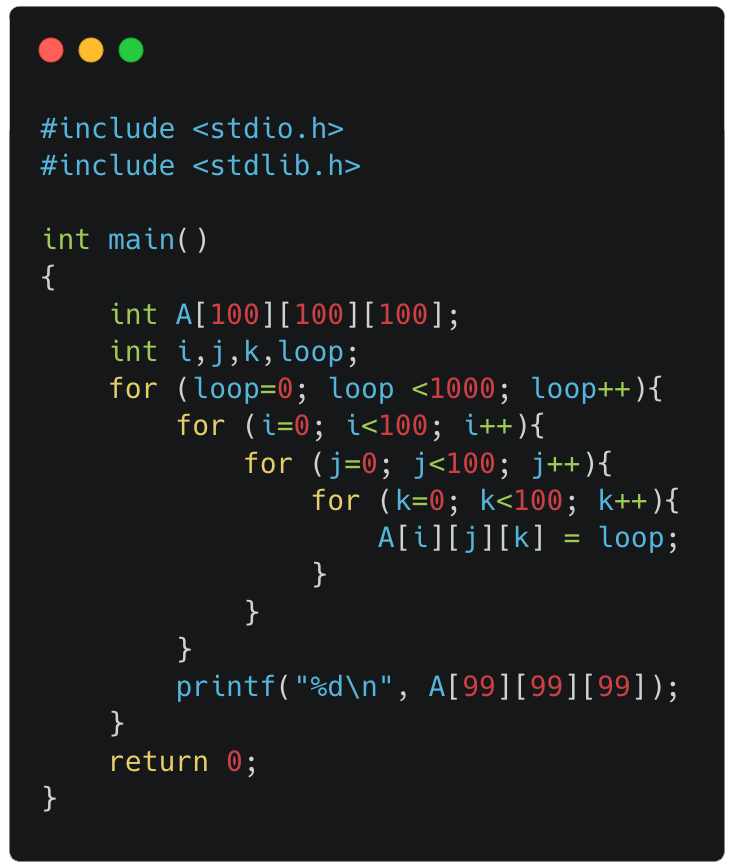
\includegraphics[angle=0,origin=t,width=38.99mm]{exempleC.png}

      \end{column}          
      \end{columns}

\end{frame}

% 
% -------------------------------------------------------------------------------------------------------------------------------------------------------
%
\begin{frame}
  \frametitle{Example (2/2)}
\vspace{3mm}

\begin{itemize}
\item \blue{C}\\
\vspace{2mm}

\begin{itemize}
\item[] \hspace{-7.75mm}\textit{without optimization} option\\
{\scriptsize
\hspace{-7.5mm}\texttt{1.286582 seconds} %991.021 ms
}
\vspace{2mm}

\item[] \hspace{-8.2mm} \textit{with optimization option } \texttt{-O3}\\
{\scriptsize
\hspace{-7.5mm}\texttt{0.087682 seconds} %85.081 ms
}
\end{itemize}
%\pause

\vspace{5mm}

\item \blue{Julia}\\
\vspace{2mm}

\begin{itemize}
\item[] \hspace{-7.75mm}\textit{1-to-1 straightforward} implementation\\
{\scriptsize
\hspace{-7.5mm}\texttt{26.732819 seconds (489.05 M allocations: 7.297 GiB, 0.29\% gc time)} %687.293 ms (23023 allocations: 8.56 MiB)
}
\vspace{-2mm}%\pause

\item[] \hspace{-7.95mm} \textit{julia style compliant} implementation\\
{\scriptsize
\hspace{-7.5mm}\texttt{0.252995 seconds (22.39 k allocations: 8.499 MiB)} %254.136 ms (22388 allocations: 8.50 MiB)
}
\vspace{2mm}%\pause

\item[] \hspace{-7.85mm} \textit{polished} implementation \\
{\scriptsize
\hspace{-7.5mm}\texttt{0.114872 seconds (20.75 k allocations: 4.318 MiB)} %95.346 ms (20747 allocations: 4.32 MiB)
}
\end{itemize}
\end{itemize}

\end{frame}

% 
% -------------------------------------------------------------------------------------------------------------------------------------------------------
%

\begin{frame}
  \frametitle{More (1/2)...}
\vspace{3mm}

{\footnotesize

Jeff Bezanson, Alan Edelman, Stefan Karpinski and Viral B. Shah.
Julia: A Fresh Approach to Numerical Computing. 
\textit{SIAM Review}, 59: 65--98. 2017.\vspace{5mm}\\

Resources:\\
\begin{itemize}
\item[] \blue{The Julia Programming Language} ( \url{https://julialang.org/}): \\
download, documentation, resources, community, etc. \vspace{4mm}
\end{itemize}

Conferences:\\
\begin{itemize}
\item[] \blue{JuliaCon Global} (\url{https://juliacon.org/}):\\ Annual International Conference since 2014 (Chicago, Cambridge, Berkeley, London, Baltimore, online, Eindhoven). \textbf{2025: Pittsburgh} \vspace{1.5mm}

\item[] \blue{JuliaCon Local} (\url{https://juliacon.org/}):\\ Annual International Conference since 2023 (Eindhoven). \textbf{2025: Paris} \vspace{1.5mm}\\

\item[] \blue{JuliaDays}:\\ the Julia \& Optimization days in France since 2019 (Nantes, Paris, Toulouse).
\end{itemize}

}
\end{frame}

% 
% -------------------------------------------------------------------------------------------------------------------------------------------------------
%

\begin{frame}
  \frametitle{More (2/2)...}
\vspace{3mm}

Example of material for optimizers:\vspace{6mm}\\
{\footnotesize

Course \vspace{2mm}\\
\quad \textbf{An introduction to Julia and JuMP for Operations Research}\\
\quad Xavier Gandibleux\\
\quad ÖGOR Summer-Workshop for PhD-candidates and Post-Docs (Krems, Austria)\\
\quad {\tiny \url{https://github.com/xgandibleux/Krems2023}}
\vspace{6mm}\\

Book \vspace{2mm}\\
\quad \textbf{Algorithms for Optimization}\\
\quad Mykel J. Kochenderfer, and Tim A. Wheeler\\
\quad The MIT Press Cambridge, Massachusetts London, England\\
\quad {\tiny \url{https://algorithmsbook.com/optimization/files/optimization.pdf}}

}
\end{frame}

% 
% -------------------------------------------------------------------------------------------------------------------------------------------------------
%

\begin{frame}
  \frametitle{Practice}
\vspace{3mm}

\begin{enumerate}
\item Installing Julia on your computer

\item Discovering the four modes of the REPL\vspace{3mm}

\item Installing the package IJulia

\item Running Julia code into Jupyter notebook\vspace{3mm}

\item Installing the Julia extension into VScode

\item Editing and running Julia code into  VScode
\end{enumerate}

\end{frame}



% ================================================================
% ================================================================
% ================================================================

\begin{frame}

\begin{center} 
{\Large \textbf{\Huge{JuMP} \vspace{5mm}} \\ Coding and Solving \\ Mathematical Programming Models \vspace{5mm}\\ \texttt{JuMP.jl}\\ }
\end{center}


              
\end{frame}

% 
% -------------------------------------------------------------------------------------------------------------------------------------------------------
%

\begin{frame}
  \frametitle{What is JuMP?}


 An Algebraic Modeling Language (AML) among the existing ones \dots
 \vspace{5mm}
\begin{center}

\includegraphics[angle=0,origin=c,height=40mm]{AML.png}
\end{center}
\vspace{5mm}

 ... for mathematical optimization (linear, mixed-integer, conic, semidefinite, nonlinear) written in the Julia language.

\end{frame}

% 
% -------------------------------------------------------------------------------------------------------------------------------------------------------
%

\begin{frame}
  \frametitle{Overview of JuMP}
\vspace{3mm}


\begin{itemize}
\item \blue{\textbf{User friendliness}}:
syntax that mimics natural mathematical expressions.
\bigskip
\pause

\item \blue{\textbf{Speed}}:
similar speeds to special-purpose modeling languages such as AMPL.
\bigskip
\pause

\item \blue{\textbf{Solver independence}}:
Currently 56 solvers are supported. \vspace{2mm}

Among the (MI)LP solvers: GLPK, Cbc, Clp, HiGHS, SCIP, CPLEX, Gurobi, FICO Xpress, COPT...
\bigskip
\pause

\item \blue{\textbf{Ease of embedding}}:
JuMP itself is written purely in Julia. Solvers are the only binary dependencies.

\end{itemize}

\end{frame}

% 
% -------------------------------------------------------------------------------------------------------------------------------------------------------
%
\begin{frame}

\begin{center} 
\Large{Getting started with JuMP}
\end{center}
              
\end{frame}

% 
% -------------------------------------------------------------------------------------------------------------------------------------------------------
%

\begin{frame}
  \frametitle{Getting started}
\vspace{3mm}


\only<1>{

  \begin{center}
    {\scriptsize
    \begin{tcolorbox}[arc=1ex, colback=black!20, colframe=black!20, left=3pt, right=3pt, top=3pt, bottom=2pt]
      \texttt{ \hspace{-1.5mm}\green{julia>}  using Pkg}\\
%%$\mbox{}$\hspace{0mm}   Pkg.add("JuMP")}
%\end{tcolorbox}  
%\vspace{1mm}
%\pause
%\begin{tcolorbox}[arc=1ex, colback=black!20, colframe=black!20, left=3pt, right=3pt, top=3pt, bottom=2pt]
      \texttt{ \hspace{-1.5mm}\green{julia>}  Pkg.add("JuMP")}
    \end{tcolorbox}  
    }
    \vspace{5mm}

    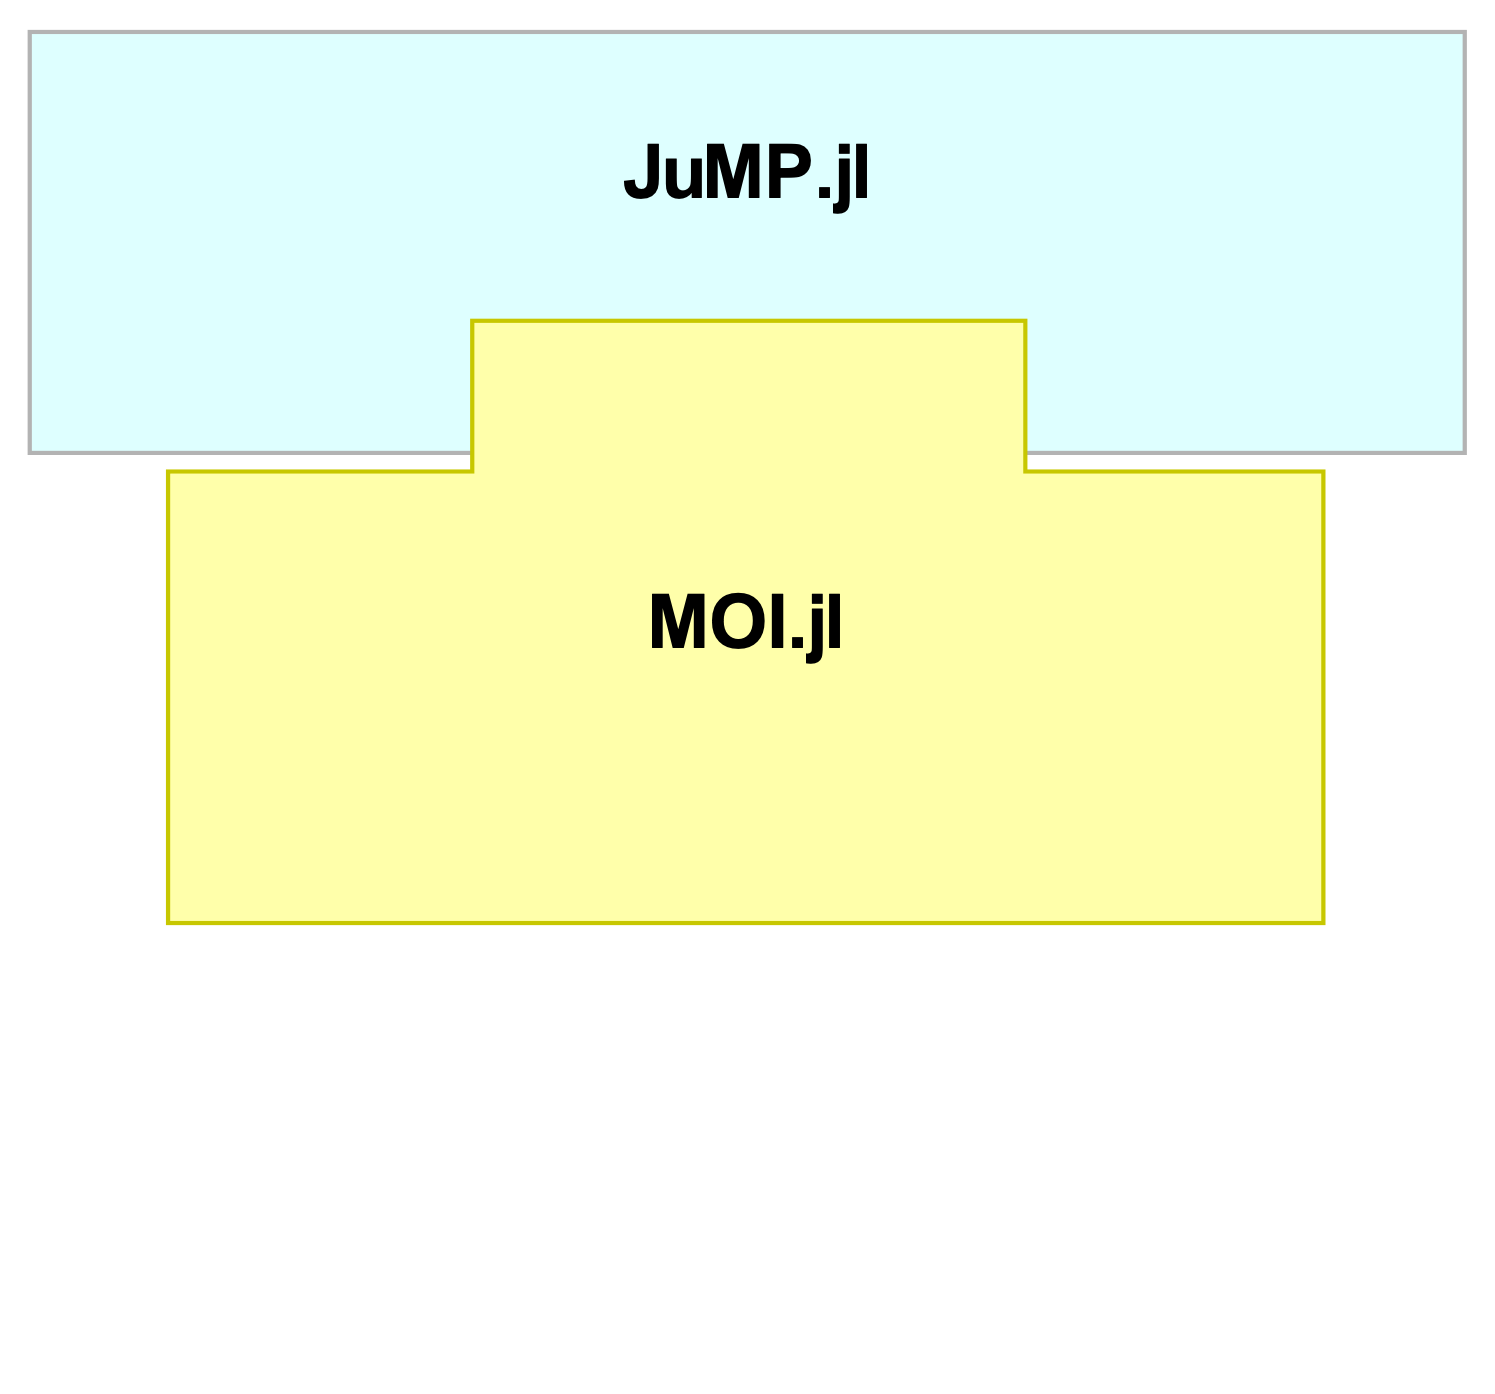
\includegraphics[angle=0,origin=c,height=55mm]{JuMP1.png}
  \end{center}

  \vspace{-15mm}
JuMP uses \textit{MathOptInterface (MOI)},  an abstraction layer designed to provide a unified interface to mathematical optimization solvers. \\
}


%\only<2>{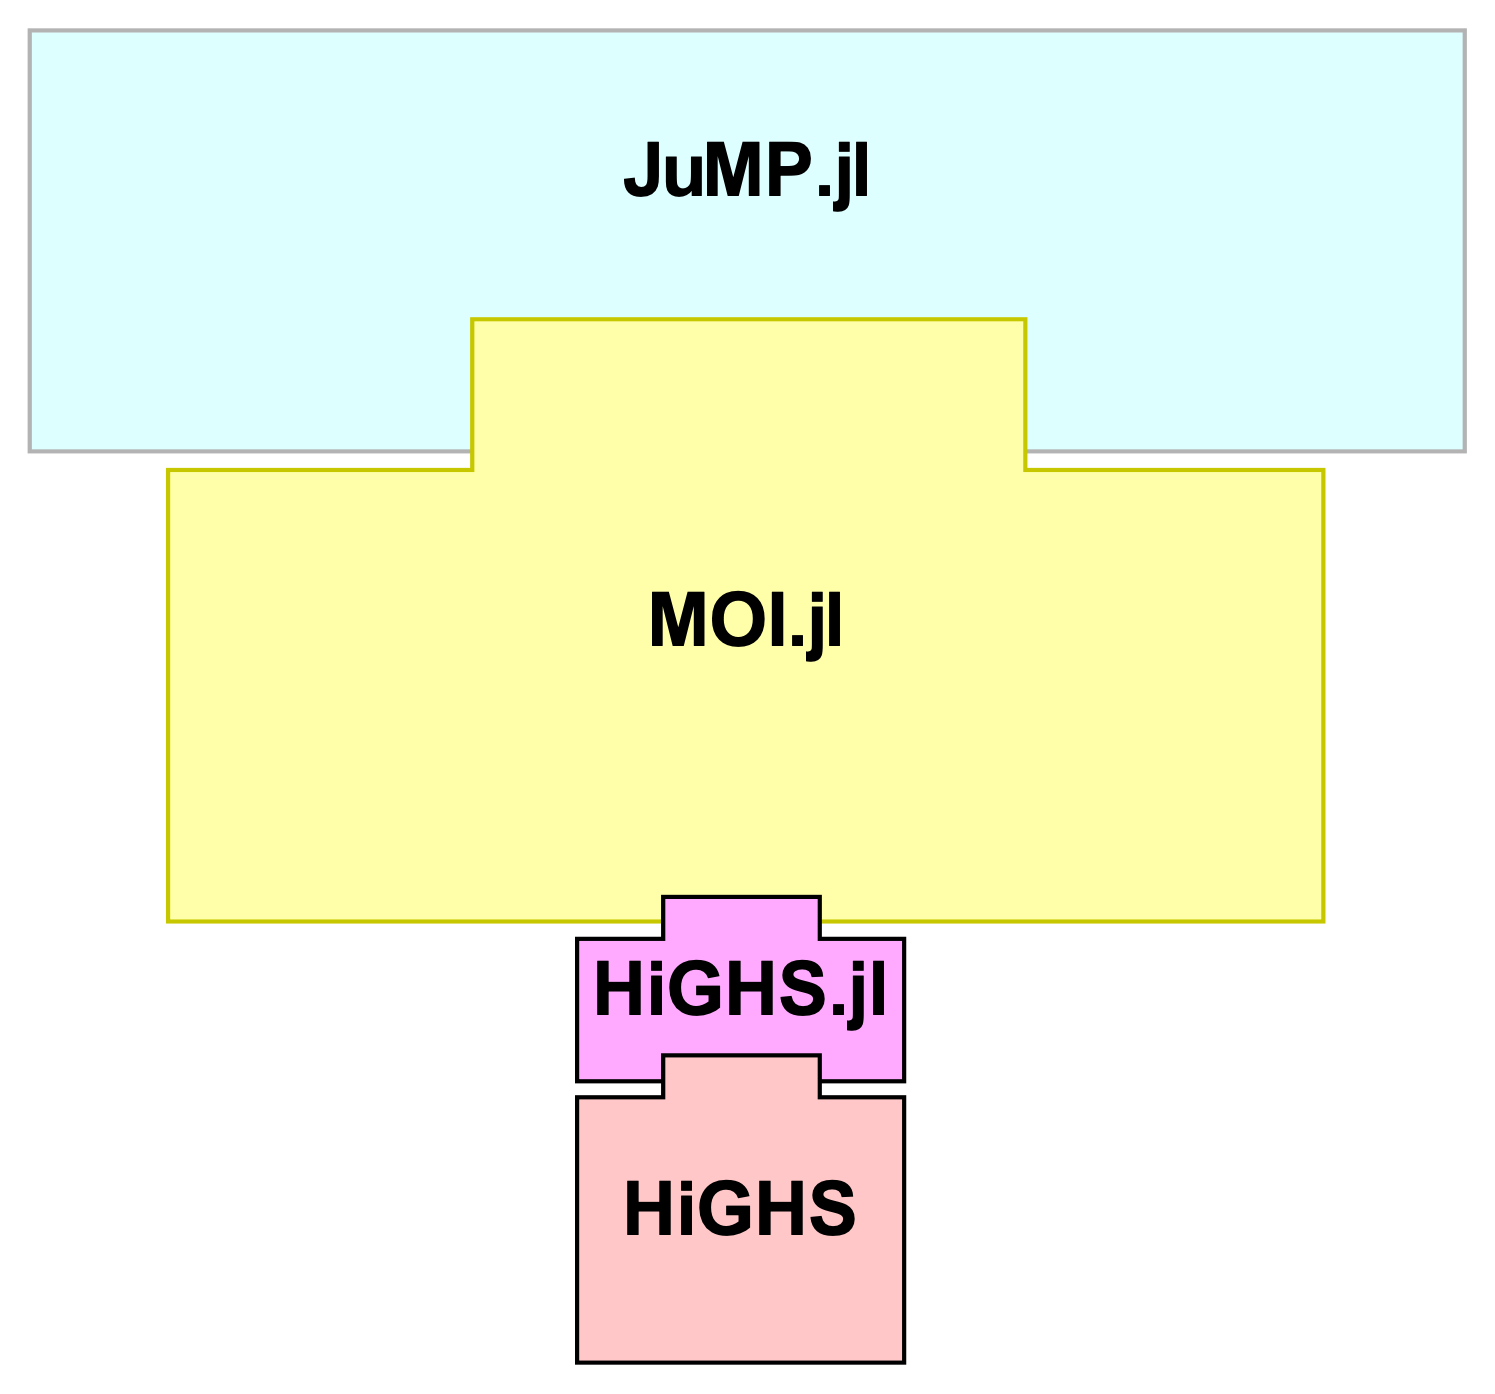
\includegraphics[angle=0,origin=c,height=55mm]{JuMP2.png}}
\only<2>{
  \begin{center}
    {\scriptsize  
      \begin{tcolorbox}[arc=1ex, colback=black!20, colframe=black!20, left=3pt, right=3pt, top=3pt, bottom=2pt]
        \texttt{ \hspace{-1.5mm}\green{julia>}   Pkg.add("HiGHS")}
      \end{tcolorbox}
    }
     \vspace{5mm}
        
    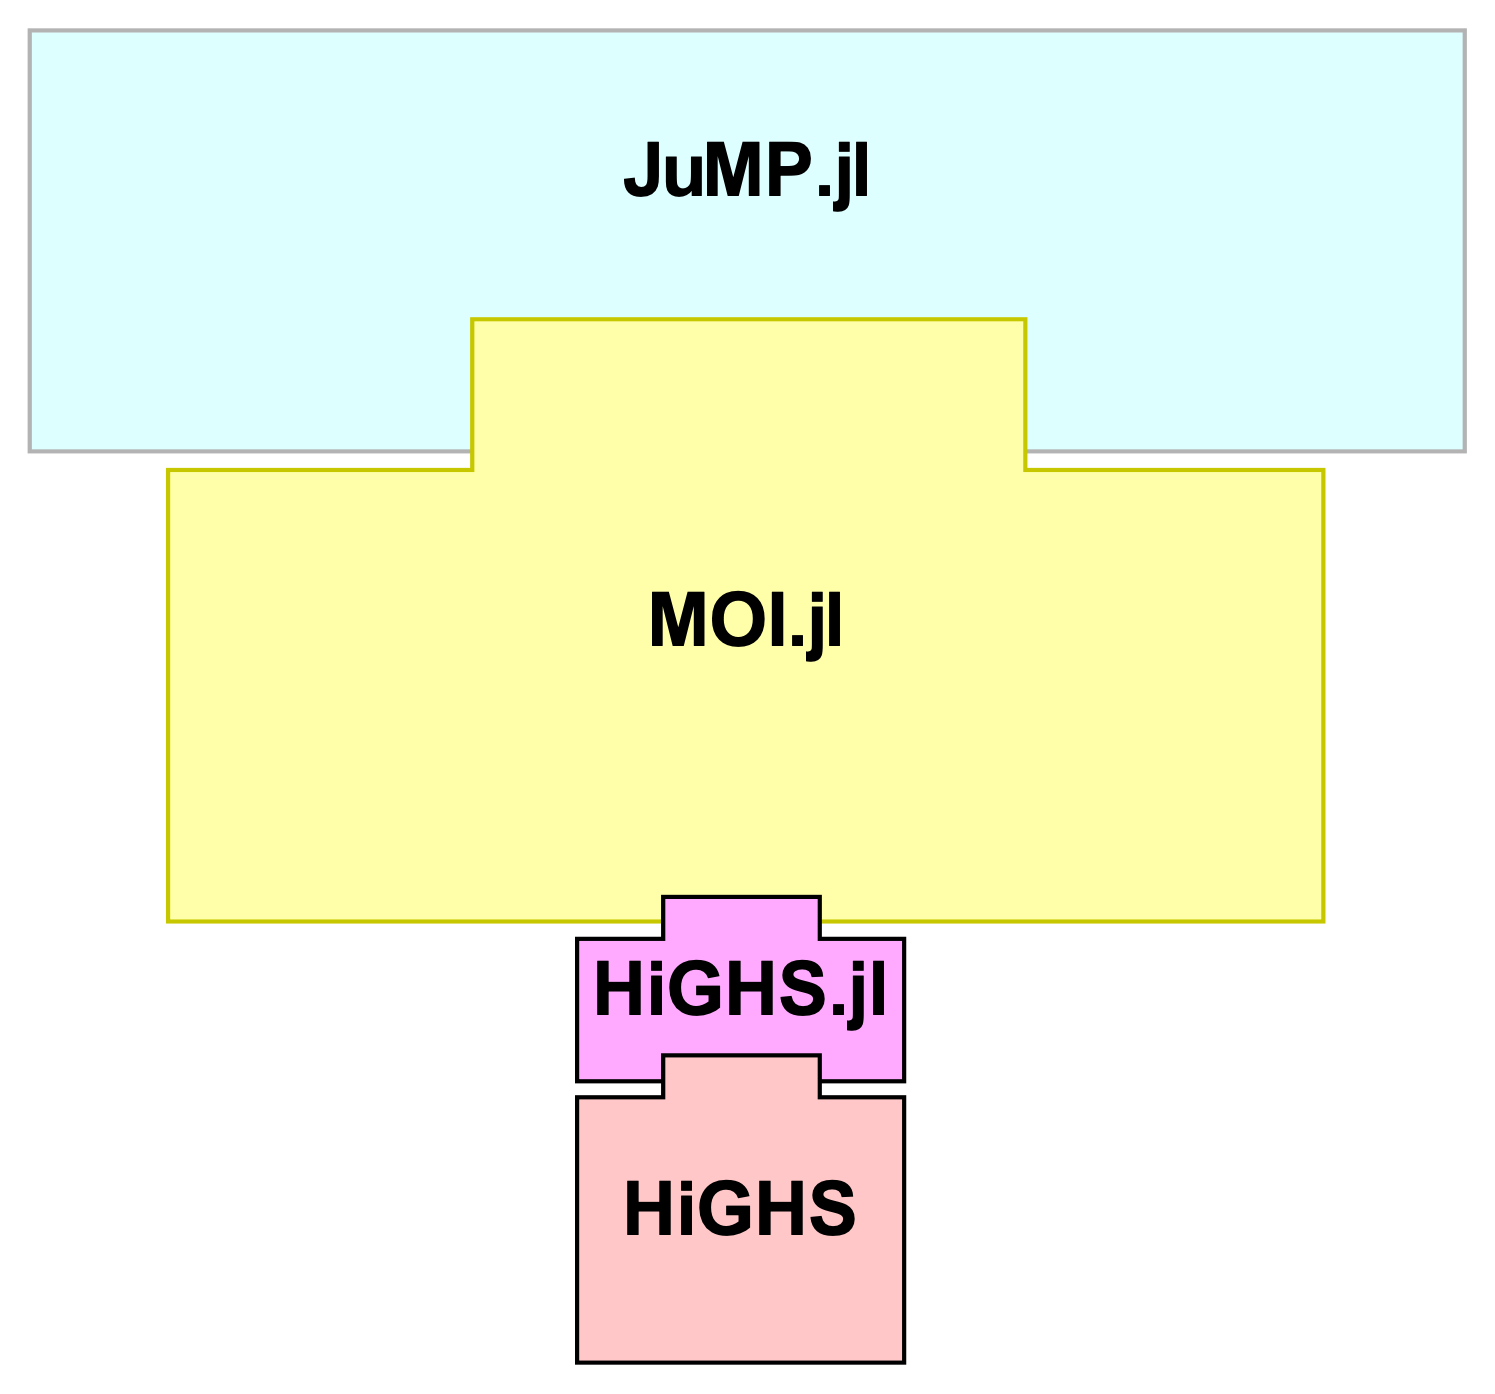
\includegraphics[angle=0,origin=c,height=55mm]{JuMP2.png}
  \end{center}
}

\only<3>{
  \begin{center}
      {\scriptsize  
      \begin{tcolorbox}[arc=1ex, colback=white, colframe=white, left=3pt, right=3pt, top=3pt, bottom=2pt]
        { \hspace{-1.5mm} With  Gurobi or CPLEX or Xpress MP solver properly installed on your computer...}
      \end{tcolorbox}
    }
     \vspace{5mm}
    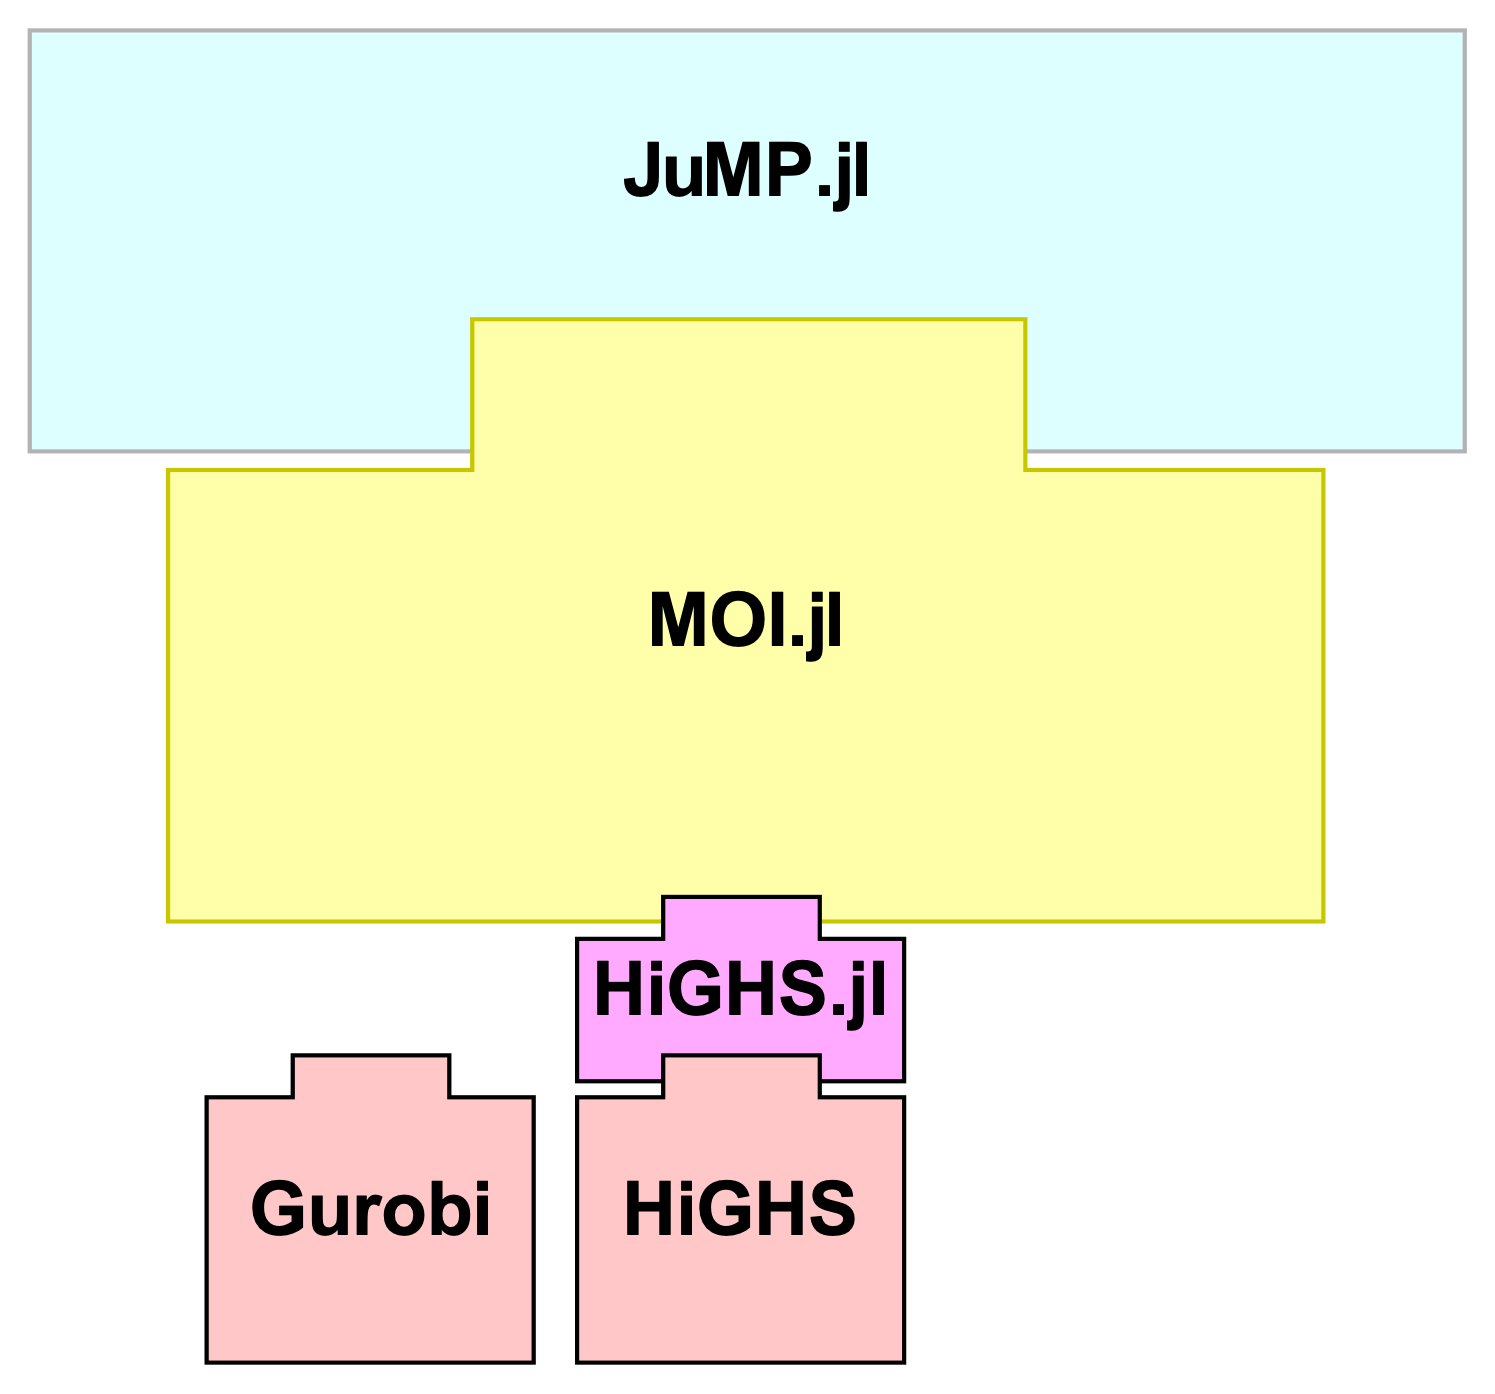
\includegraphics[angle=0,origin=c,height=55mm]{JuMP3.png}
  \end{center}
}

\only<4>{
  \begin{center}
    {\scriptsize  
      \begin{tcolorbox}[arc=1ex, colback=black!20, colframe=black!20, left=3pt, right=3pt, top=3pt, bottom=2pt]
        \texttt{ \hspace{-1.5mm}\green{julia>}   Pkg.add("Gurobi")}
      \end{tcolorbox}
    }
     \vspace{5mm}
        
    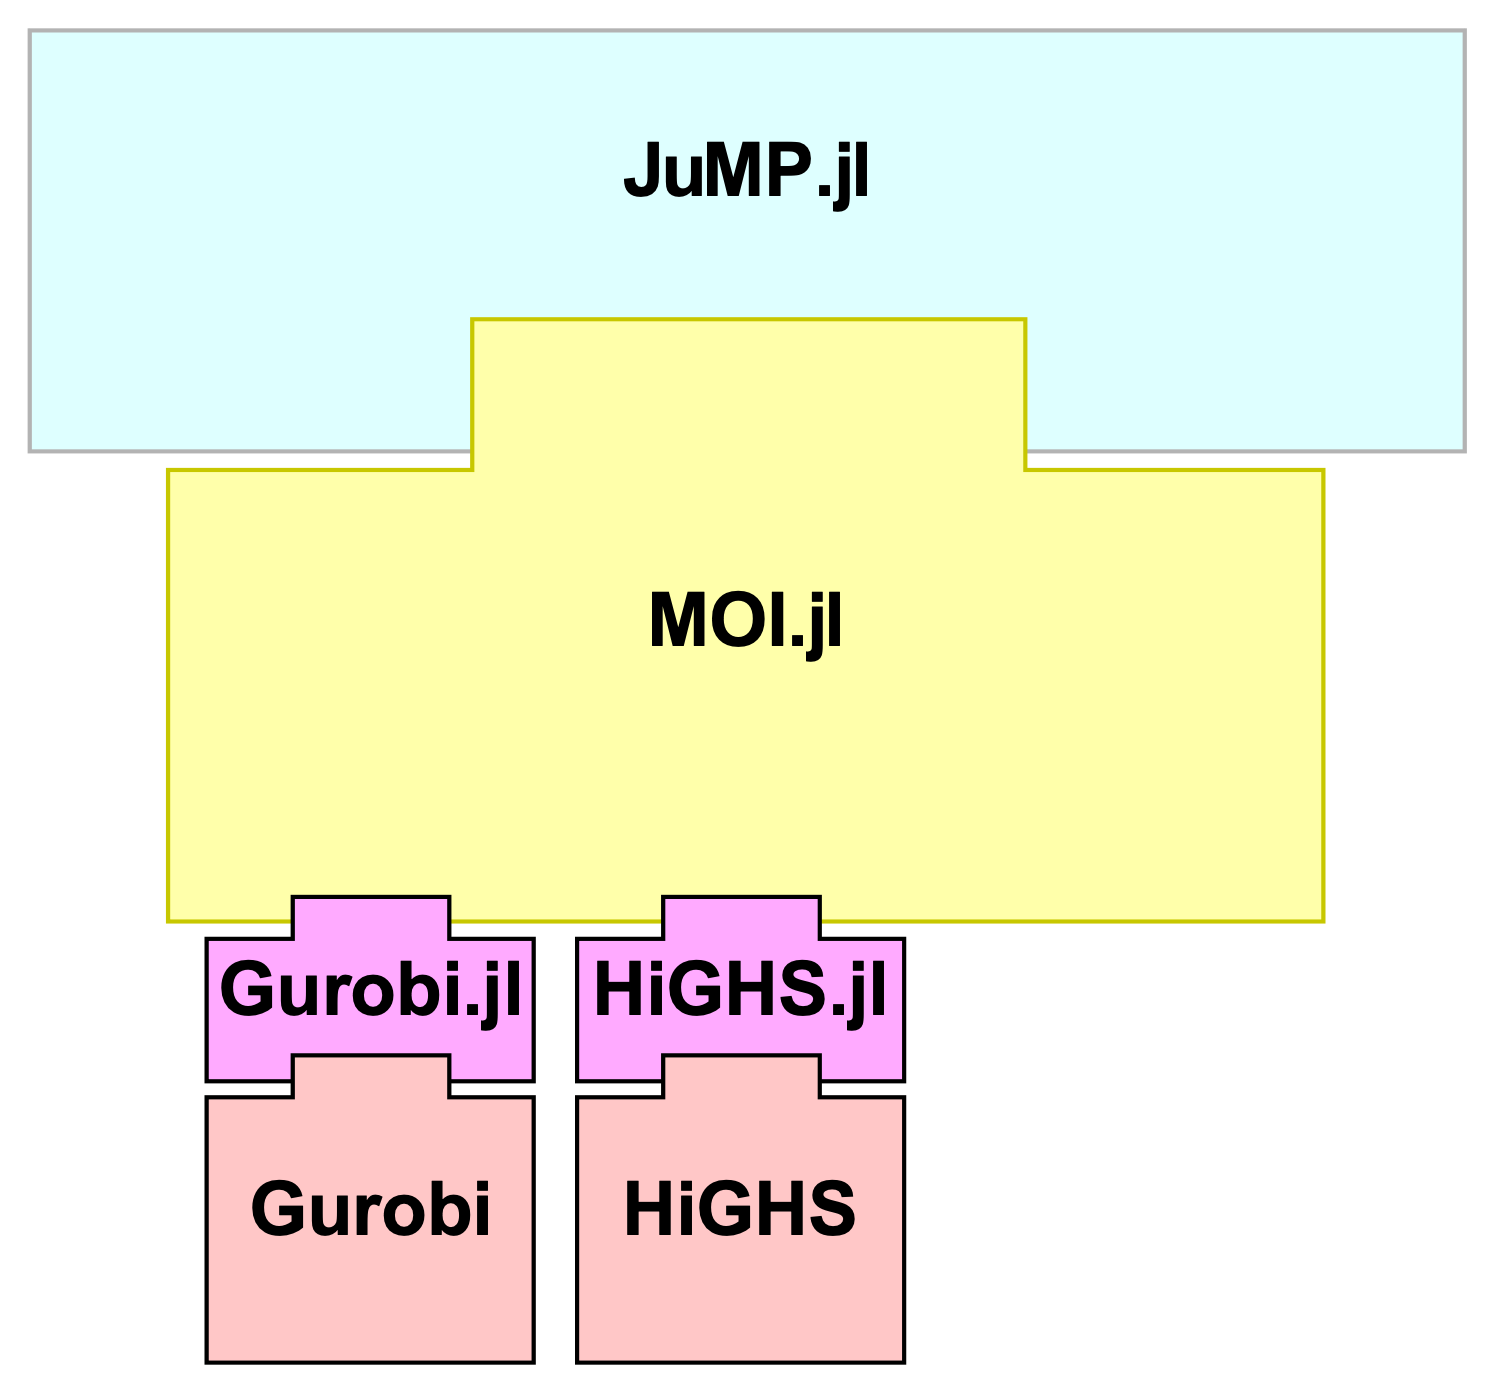
\includegraphics[angle=0,origin=c,height=55mm]{JuMP4.png}
  \end{center}
}


%\only<4>{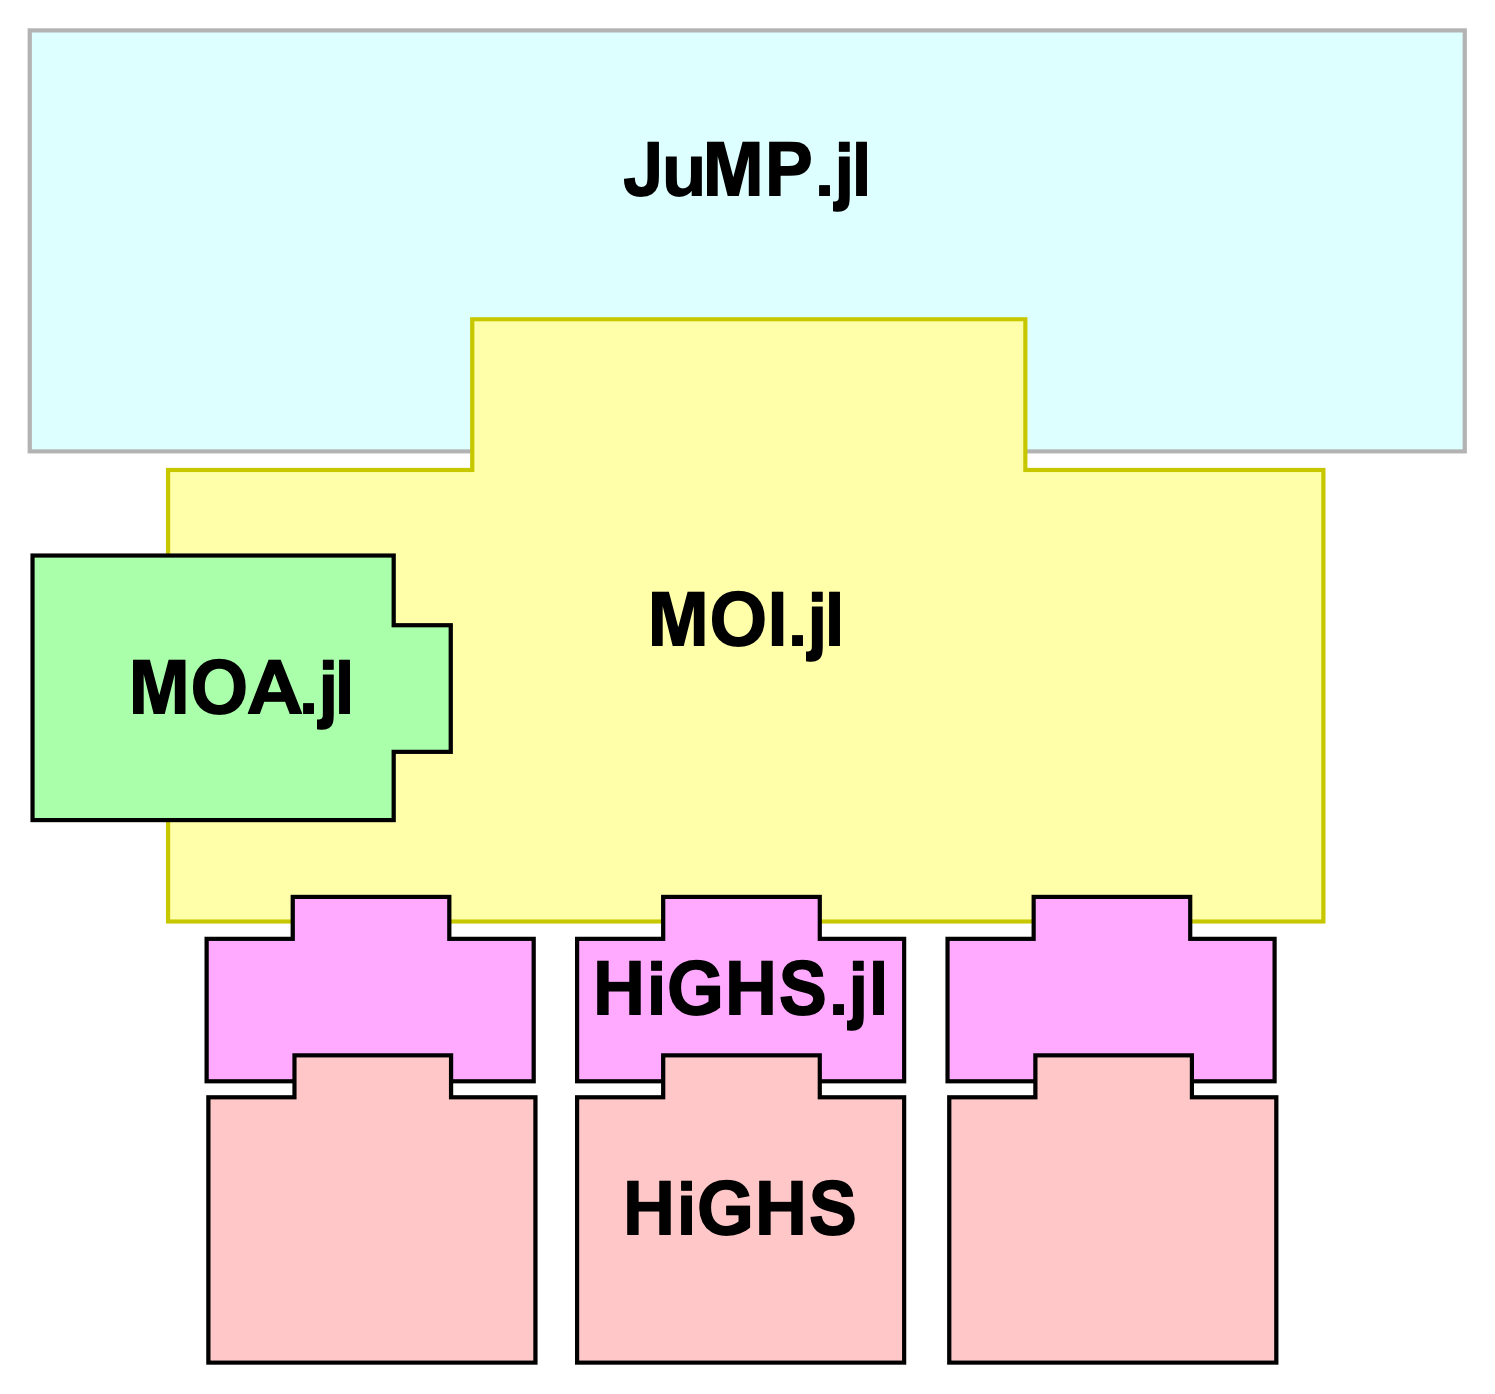
\includegraphics[angle=0,origin=c,height=55mm]{JuMP5.png}}


\end{frame}

%% 
%% -------------------------------------------------------------------------------------------------------------------------------------------------------
%%
%
%\begin{frame}
%  \frametitle{Getting Started}
%\vspace{3mm}
%
%\hspace{-2mm}Install:
%\vspace{1mm}
%{\scriptsize
%\begin{tcolorbox}[arc=1ex, colback=black!20, colframe=black!20, left=3pt, right=3pt, top=3pt, bottom=2pt]
%\texttt{ \hspace{-1.5mm}\green{julia>}  using Pkg}
%%$\mbox{}$\hspace{0mm}   Pkg.add("JuMP")}
%\end{tcolorbox}  
%\vspace{1mm}
%\pause
%\begin{tcolorbox}[arc=1ex, colback=black!20, colframe=black!20, left=3pt, right=3pt, top=3pt, bottom=2pt]
%\texttt{ \hspace{-1.5mm}\green{julia>}  Pkg.add("JuMP")}
%\end{tcolorbox}  
%\vspace{1mm}
%\pause
%
%\vspace{1mm}
%%\pause
%\vspace{3mm}
%}
%
%
%\end{frame}
%
%
%% 
%% -------------------------------------------------------------------------------------------------------------------------------------------------------
%%
%
%\begin{frame}
%  \frametitle{Getting started}
%\vspace{3mm}
%
%\hspace{-2mm}Install:
%\vspace{1mm}
%\begin{tcolorbox}[arc=1ex, colback=blue!20, colframe=blue!20, left=3pt, right=3pt, top=3pt, bottom=2pt]
%\texttt{ \hspace{-2mm}  using Pkg\\
%$\mbox{}$\hspace{0mm}   Pkg.add("JuMP")}
%\end{tcolorbox}  
%\vspace{1mm}
%\pause
%\begin{tcolorbox}[arc=1ex, colback=blue!20, colframe=blue!20, left=3pt, right=3pt, top=3pt, bottom=2pt]
%\texttt{ \hspace{-2mm}  Pkg.add("GLPK")}
%\end{tcolorbox}
%\pause
%\vspace{3mm}
%
%\hspace{-2mm}Setup:
%\vspace{1mm}
%\begin{tcolorbox}[arc=1ex, colback=blue!20, colframe=blue!20, left=3pt, right=3pt, top=3pt, bottom=2pt]
%\texttt{ \hspace{-2mm}  using JuMP}
%\end{tcolorbox}  
%\vspace{1mm}
%\begin{tcolorbox}[arc=1ex, colback=blue!20, colframe=blue!20, left=3pt, right=3pt, top=3pt, bottom=2pt]
%\texttt{ \hspace{-2mm}  using GLPK}
%\end{tcolorbox}  
%\vspace{1mm}
%
%\end{frame}
%


% 
% -------------------------------------------------------------------------------------------------------------------------------------------------------
%
\begin{frame}

\begin{center} 
\Large{Modeling and solving a (MI)LP with JuMP}
\end{center}
              
\end{frame}

% 
% -------------------------------------------------------------------------------------------------------------------------------------------------------
%

\begin{frame}
  \frametitle{The optimization problem}
\vspace{3mm}


$$\quad \left[ \ \begin{array}{crcrccc}
\quad  \max z(x) = & x_1 &+& 3x_2 &   &    & \quad (0)\quad \  \\
\quad  s.t &         x_1 &+&  x_2 &\le& 14 & \quad (1)\quad \ \\
    &       -2x_1 &+& 3x_2 &\le& 12 & \quad (2)\quad \ \\
    &        2x_1 &-&  x_2 &\le& 12 & \quad (3)\quad \ \\
    &         x_1 &,&  x_2 &\ge& 0  & \quad (4)\quad \
 \end{array}\ \right]
$$

\end{frame}

% using JuMP
% using GLPK
% model = Model(GLPK.Optimizer)
% @variable(model, x1 >= 0)
% @variable(model, x2 >= 0)
% @objective(model, Max, x1 + 3x2)
% @constraint(model, cst1, x1 + x2 <= 14)
% @constraint(model, cst2, -2x1 + 3x2 <= 12)
% @constraint(model, cst3, 2x1 - x2 <= 12)
% print(model)
% optimize!(model)
% @show termination_status(model)
% @show primal_status(model)
% @show dual_status(model)
% @show objective_value(model)
% @show value(x1)
% @show value(x2)
% @show shadow_price(cst1)
% @show shadow_price(cst2)
% @show shadow_price(cst3)
 
 % 
% -------------------------------------------------------------------------------------------------------------------------------------------------------
%

\begin{frame}
  \frametitle{Declaring  the packages to use}
\vspace{3mm}

 {
\begin{tcolorbox}[arc=1ex, colback=black!20, colframe=black!20, left=3pt, right=3pt, top=3pt, bottom=2pt]
\texttt{ \hspace{-1.5mm}\green{julia>}  using JuMP, HiGHS}
\end{tcolorbox} 
}

\end{frame}

% 
% -------------------------------------------------------------------------------------------------------------------------------------------------------
%

\begin{frame}
  \frametitle{Coding the optimization problem (1/4)}
\vspace{3mm}


\hspace{-2mm} Creating a model:
\vspace{1mm}
\begin{tcolorbox}[arc=1ex, colback=yellow!20, colframe=yellow!20, left=3pt, right=3pt, top=3pt, bottom=2pt]
\texttt{ \hspace{-2mm} \textit{modelId} = Model( )}
\end{tcolorbox}
\begin{tcolorbox}[arc=1ex, colback=black!20, colframe=black!20, left=3pt, right=3pt, top=3pt, bottom=2pt]
\texttt{ \hspace{-2mm}\greenxg{julia>}  modLP = Model( )}
\end{tcolorbox} 
\vspace{8mm}

\hspace{-2mm} Result:
\vspace{1mm}
{\tiny
{
$$\quad \left[ \ \begin{array}{crcrccc}
\mbox{ } \hspace{35mm} \mbox{ } \\
\mbox{ } \\
\mbox{ } \\
\mbox{ } \\
\mbox{ } 
 \end{array}\ \right]
$$
}
}



\end{frame}

% 
% -------------------------------------------------------------------------------------------------------------------------------------------------------
%

\begin{frame}
  \frametitle{Coding the optimization problem (2/4)}
\vspace{3mm}

\hspace{-2mm} Defining a variable:
\vspace{1mm}
\begin{tcolorbox}[arc=1ex, colback=yellow!20, colframe=yellow!20, left=3pt, right=3pt, top=3pt, bottom=2pt]
\texttt{ \hspace{-2mm} @variable(\textit{modelId}, \textit{variable})}
\end{tcolorbox}
\begin{tcolorbox}[arc=1ex, colback=black!20, colframe=black!20, left=3pt, right=3pt, top=3pt, bottom=2pt]
\texttt{ \hspace{-2mm}\greenxg{julia>}  @variable(modLP, x1 >= 0)} \\
%\end{tcolorbox} 
%%
%\begin{tcolorbox}[arc=1ex, colback=black!20, colframe=black!20, left=3pt, right=3pt, top=3pt, bottom=2pt]
\texttt{ \hspace{-2mm}\greenxg{julia>}  @variable(modLP, x2 >= 0)}
\end{tcolorbox} 
\vspace{8mm}

\hspace{-2mm} Result:
\vspace{1mm}
{\tiny
{
$$\quad \left[ \ \begin{array}{crcrccc}
\mbox{ } \hspace{19mm} \\
\mbox{ } \\
\mbox{ } \\
\mbox{ } \\
    &         x_1 &,&  x_2 &\ge& 0  & \quad (4)\quad \
 \end{array}\ \right]
$$
}
}





\end{frame}

% 
% -------------------------------------------------------------------------------------------------------------------------------------------------------
%

\begin{frame}
  \frametitle{Coding the optimization problem (3/4)}
\vspace{3mm}


\hspace{-2mm} Defining an objective function:
\vspace{1mm}
\begin{tcolorbox}[arc=1ex, colback=yellow!20, colframe=yellow!20, left=3pt, right=3pt, top=3pt, bottom=2pt]
\texttt{ \hspace{-2mm} @objective(\textit{modelId}, \textit{sense}, \textit{function})}
\end{tcolorbox}
\begin{tcolorbox}[arc=1ex, colback=black!20, colframe=black!20, left=3pt, right=3pt, top=3pt, bottom=2pt]
\texttt{ \hspace{-2mm}\greenxg{julia>}  @objective(modLP, Max, x1 + 3x2)}
\end{tcolorbox} 
\vspace{8mm}

\hspace{-2mm} Result:
\vspace{1mm}
{\tiny
{
$$\quad \left[ \ \begin{array}{crcrccc}
\quad  \max z(x) = \qquad & x_1 &+& 3x_2 &   &    & \quad (0)\quad \  \\
\mbox{ } \\
\mbox{ } \\
\mbox{ } \\
    &         x_1 &,&  x_2 &\ge& 0  & \quad (4)\quad \
 \end{array}\ \right]
$$
}
}


\end{frame}


% 
% -------------------------------------------------------------------------------------------------------------------------------------------------------
%

\begin{frame}
  \frametitle{Coding the optimization problem (4/4)}
\vspace{1mm}


\hspace{-2mm} Defining a constraint:
\vspace{1mm}
\begin{tcolorbox}[arc=1ex, colback=yellow!20, colframe=yellow!20, left=3pt, right=3pt, top=3pt, bottom=2pt]
\texttt{ \hspace{-2mm} @constraint(\textit{modelId}, \textit{id}, \textit{constraint})}
\end{tcolorbox}
\begin{tcolorbox}[arc=1ex, colback=black!20, colframe=black!20, left=3pt, right=3pt, top=3pt, bottom=2pt]
\texttt{ \hspace{-2mm}\greenxg{julia>}  @constraint(modLP, cst1, x1 + x2 <= 14)}\\
%\end{tcolorbox} 
%\begin{tcolorbox}[arc=1ex, colback=black!20, colframe=black!20, left=3pt, right=3pt, top=3pt, bottom=2pt]
\texttt{ \hspace{-2mm}\greenxg{julia>}  @constraint(modLP, cst2, -2x1 + 3x2 <= 12)}\\
%\end{tcolorbox} 
%\begin{tcolorbox}[arc=1ex, colback=black!20, colframe=black!20, left=3pt, right=3pt, top=3pt, bottom=2pt]
\texttt{ \hspace{-2mm}\greenxg{julia>}  @constraint(modLP, cst3, 2x1 - x2 <= 12)}
\end{tcolorbox} 
\vspace{8mm}

\hspace{-2mm} Result:
\vspace{1mm}
{\tiny
{
$$\quad \left[ \ \begin{array}{crcrccc}
\quad  \max z(x) = & x_1 &+& 3x_2 &   &    & \quad (0)\quad \  \\
\quad  s.t &         x_1 &+&  x_2 &\le& 14 & \quad (1)\quad \ \\
    &       -2x_1 &+& 3x_2 &\le& 12 & \quad (2)\quad \ \\
    &        2x_1 &-&  x_2 &\le& 12 & \quad (3)\quad \ \\
    &         x_1 &,&  x_2 &\ge& 0  & \quad (4)\quad \
 \end{array}\ \right]
$$
}
}


\end{frame}




% 
% -------------------------------------------------------------------------------------------------------------------------------------------------------
%

\begin{frame}
  \frametitle{Solving  the optimization problem}
\vspace{1mm}

\vspace{1mm}
\begin{tcolorbox}[arc=1ex, colback=yellow!20, colframe=yellow!20, left=3pt, right=3pt, top=3pt, bottom=2pt]
\texttt{ \hspace{-2mm} set\_optimizer(\textit{modelId}, \textit{solver} )}
\end{tcolorbox}
\begin{tcolorbox}[arc=1ex, colback=black!20, colframe=black!20, left=3pt, right=3pt, top=3pt, bottom=2pt]
\texttt{ \hspace{-2mm}\greenxg{julia>}  set\_optimizer(modLP, HiGHS.Optimizer)}
\end{tcolorbox} 
\vspace{2mm}

\vspace{1mm}
\begin{tcolorbox}[arc=1ex, colback=yellow!20, colframe=yellow!20, left=3pt, right=3pt, top=3pt, bottom=2pt]
\texttt{ \hspace{-2mm} set\_silent(\textit{modelId} )}
\end{tcolorbox}
\begin{tcolorbox}[arc=1ex, colback=black!20, colframe=black!20, left=3pt, right=3pt, top=3pt, bottom=2pt]
\texttt{ \hspace{-2mm}\greenxg{julia>}  set\_silent(modLP)}
\end{tcolorbox} 
\vspace{2mm}



%\hspace{-2mm} Defining Constraints:
\vspace{1mm}
\begin{tcolorbox}[arc=1ex, colback=yellow!20, colframe=yellow!20, left=3pt, right=3pt, top=3pt, bottom=2pt]
\texttt{ \hspace{-2mm} optimize!(\textit{modelId})}
\end{tcolorbox}
\begin{tcolorbox}[arc=1ex, colback=black!20, colframe=black!20, left=3pt, right=3pt, top=3pt, bottom=2pt]
\texttt{ \hspace{-2mm}\greenxg{julia>}  optimize!(modLP)}
\end{tcolorbox} 
\vspace{3mm}


\end{frame}

% 
% -------------------------------------------------------------------------------------------------------------------------------------------------------
%

\begin{frame}
  \frametitle{Querying the result}
\vspace{1mm}


%\hspace{-2mm} Defining Constraints:
%\vspace{1mm}
%\begin{tcolorbox}[arc=1ex, colback=yellow!20, colframe=yellow!20, left=3pt, right=3pt, top=3pt, bottom=2pt]
%\texttt{ \hspace{-2mm} optimize!(\textit{modName})}
%\end{tcolorbox}
\begin{tcolorbox}[arc=1ex, colback=black!20, colframe=black!20, left=3pt, right=3pt, top=3pt, bottom=2pt]
\texttt{ \hspace{-2mm}\greenxg{julia>}  @show is\_solved\_and\_feasible(modLP)}
%\texttt{ \hspace{-2mm}\greenxg{julia>}  @show primal\_status(model)} %\\
% \texttt{ \hspace{-2mm}\greenxg{julia>}  @show dual\_status(model)}
 \end{tcolorbox} 
 \medskip
\begin{tcolorbox}[arc=1ex, colback=black!20, colframe=black!20, left=3pt, right=3pt, top=3pt, bottom=2pt]
\texttt{ \hspace{-2mm}\greenxg{julia>}  @show termination\_status(modLP)}
%\texttt{ \hspace{-2mm}\greenxg{julia>}  @show primal\_status(model)} %\\
% \texttt{ \hspace{-2mm}\greenxg{julia>}  @show dual\_status(model)}
 \end{tcolorbox} 
 \medskip
 \pause
 \begin{tcolorbox}[arc=1ex, colback=black!20, colframe=black!20, left=3pt, right=3pt, top=3pt, bottom=2pt]
\texttt{ \hspace{-2mm}\greenxg{julia>}   @show objective\_value(modLP)}
 \end{tcolorbox} 
 \medskip
 \pause
 \begin{tcolorbox}[arc=1ex, colback=black!20, colframe=black!20, left=3pt, right=3pt, top=3pt, bottom=2pt]
\texttt{ \hspace{-2mm}\greenxg{julia>}   @show value(x1)}\\
\texttt{ \hspace{-2mm}\greenxg{julia>}   @show value(x2)}
 \end{tcolorbox} 
 \medskip
% \pause
%\begin{tcolorbox}[arc=1ex, colback=black!20, colframe=black!20, left=3pt, right=3pt, top=3pt, bottom=2pt]
%\texttt{ \hspace{-2mm}\greenxg{julia>}   @show dual(cst1)}\\
%\texttt{ \hspace{-2mm}\greenxg{julia>}   @show dual(cst2)}\\
%\texttt{ \hspace{-2mm}\greenxg{julia>}   @show dual(cst3)}
%\end{tcolorbox} 
% \pause
%\begin{tcolorbox}[arc=1ex, colback=black!20, colframe=black!20, left=3pt, right=3pt, top=3pt, bottom=2pt]
%\texttt{ \hspace{-2mm}\greenxg{julia>}   solution\_summary(model)}
%\end{tcolorbox} 


\end{frame}

% 
% -------------------------------------------------------------------------------------------------------------------------------------------------------
%

\begin{frame}
  \frametitle{Summary (explicit model)}
\vspace{1mm}

{\scriptsize
\begin{tcolorbox}[arc=1ex, colback=black!20, colframe=black!20, left=3pt, right=3pt, top=3pt, bottom=2pt]
\texttt{ \hspace{-1.5mm}\green{julia>}  using JuMP, HiGHS}\medskip \\
\texttt{ \hspace{-2mm}\greenxg{julia>}  modLP = Model( )}\\
\texttt{ \hspace{-2mm}\greenxg{julia>}  @variable(modLP, x1 >= 0)} \\
\texttt{ \hspace{-2mm}\greenxg{julia>}  @variable(modLP, x2 >= 0)}\\
\texttt{ \hspace{-2mm}\greenxg{julia>}  @objective(modLP, Max, x1 + 3x2)}\\
\texttt{ \hspace{-2mm}\greenxg{julia>}  @constraint(modLP, cst1, x1 + x2 <= 14)}\\
\texttt{ \hspace{-2mm}\greenxg{julia>}  @constraint(modLP, cst2, -2x1 + 3x2 <= 12)}\\
\texttt{ \hspace{-2mm}\greenxg{julia>}  @constraint(modLP, cst3, 2x1 - x2 <= 12)}\medskip \\
\texttt{ \hspace{-2mm}\greenxg{julia>}  set\_optimizer(modLP, HiGHS.Optimizer)}\\
\texttt{ \hspace{-2mm}\greenxg{julia>}  set\_silent(modLP)} \\
\texttt{ \hspace{-2mm}\greenxg{julia>}  optimize!(modLP)}\medskip \\
\texttt{ \hspace{-2mm}\greenxg{julia>}  @show is\_solved\_and\_feasible(modLP)}\\
\texttt{ \hspace{-2mm}\greenxg{julia>}   @show objective\_value(modLP)}\\
\texttt{ \hspace{-2mm}\greenxg{julia>}   @show value(x1), value(x2)}
 \end{tcolorbox} 
 }
 
\end{frame}

%
%-----------------------------------------------------------
%
\begin{frame}
  \frametitle{More...}
\vspace{3mm}

{\footnotesize

 Miles Lubin, Oscar Dowson, Joaquim {Dias Garcia}, Joey Huchette, Beno{\^i}t Legat, Juan Pablo Vielma.
{JuMP} 1.0: {R}ecent improvements to a modeling language for mathematical optimization.
\textit{Mathematical Programming Computation}. 2023.\vspace{5mm}\\

Miles Lubin. 
The state of JuMP. 
\textit{JuMP-dev 2024 - Co-Located with ISMP'2024}, July 19-21, 2024. GERAD research center, Montréal, Canada.\\
\url{https://www.youtube.com/watch?v=cMUTdfoAMpo} \vspace{5mm}\\


Resources:\\
\begin{itemize}
\item[] \blue{The JuMP website} (\url{https://jump.dev/}):\\
documentation, resources, community, etc. \vspace{4mm}
\end{itemize}

Workshops:\\
\begin{itemize}
\item[] \blue{JuMP-dev} (\url{https://jump.dev/meetings/jumpdev2025/}): \\
Regular meeting since 2017: Cambridge (USA), Bordeaux (France), Santiago (Chile), online, Montréal (Canada). \textbf{2025: Auckland (New Zealand)} %\vspace{1.5mm}
\end{itemize}
}
   
\end{frame}

% 
% -------------------------------------------------------------------------------------------------------------------------------------------------------
%

\begin{frame}
  \frametitle{Practice}
\vspace{3mm}

\begin{enumerate}
\item Installing the packages JuMP and HiGHS

\item Coding and solving a IP problem \vspace{3mm}

\end{enumerate}

\end{frame}


% ================================================================
% ================================================================
% ================================================================

\begin{frame}

\begin{center} 
{\Large \textbf{\Huge{MOA} \vspace{5mm}} \\ Moving from \\ single to multiple objectives MIP optimization \vspace{5mm}\\ \texttt{MultiObjectiveAlgorithms.jl} \\}
\end{center}

%\vspace{8mm}



      
\end{frame}



% 
% -------------------------------------------------------------------------------------------------------------------------------------------------------
%
\begin{frame}[fragile]
  \frametitle{Multiobjective Optimization Problem (MOP) notations}

\[
\begin{array}{clrclrrrl}
\min   & \red{F}(x)   \\
s.t.     & x  \ \in \ X
\end{array}
\]


\vspace{-2mm}
\noindent 
where:
\vspace{2mm}
%\vfill
$$
\begin{array}{rcl}
%
X \subseteq\mR^n  & \longrightarrow & \hbox{the set of feasible solutions}\\
Y=F(X)\subseteq \mR^{\red{p}} & \longrightarrow & \hbox{the set of images}\\
\notag
\end{array}
$$
%\pause

\hspace{0mm}Computing sets $\textcolor{blue}{X_E}$  and $\textcolor{blue}{Y_N}$ for MOP:

\vspace{0mm}

\begin{center}
{$y=F(x)$\medskip\\
$y^*\in Y$ is \textcolor{black}{nondominated}, if $\not\exists\, y\in Y$ such that $y_i\leq y^*_i,~\forall i$ and $ y\not= y^*$.\\
			$\textcolor{blue}{Y_N}$ is the set of nondominated points.\medskip\\
			$x^*\in X$ is \textcolor{black}{efficient} if $y^*$ is nondominated.\\
			$\textcolor{blue}{X_E}$ is a complete set of efficient solutions.}

\end{center}
\vspace{5mm}


\end{frame}


%
% ================================================================
% 
%\setwatermark{}
%\setwatermark{\fontsize{125pt}{125pt}\selectfont{Simple}}
\begin{frame}{Examples of $Y$ and $Y_N$ when $p=2$}

\hspace{-3mm}Computing \textcolor{blue}{$Y_N$} for Multiobjective (linear) Optimization Problems ({MOP}):
\vspace{-10mm}

\begin{columns}
% ----------------------------------------------------------------------------------------------------------------
\column{0.33\textwidth}
  \begin{center}
  $${x} \ {\in} \ {\mR^{n_1}}\vspace{0mm}$$
  \end{center}
  \begin{tikzpicture}[scale=0.35, label distance= 0.2mm, inner sep= 0.1mm]
	\draw[help lines] (0,0) grid (9,9);
	\draw[->] (0,0) -- (9,0);
	\draw[->] (0,0) -- (0,9);
	\node at ($(0,0)!.95!-3:(9,0)$) {$f^1$};
	\node at ($(0,0)!.95!3:(0,9)$) {$f^2$};

\onslide<1->{
	\draw[color=gray, fill = gray!20] (2,8) -- (1,7)-- (2,5) -- (4,3) -- (7,1) -- (8,3) -- (7,6) -- (5.5,7.5) -- (4,8.5) -- (2,8);
 %        \draw[color=red] 	(1,7)-- (2,5) -- (4,3) -- (7,1);
}
\only<2>{
	\draw[blue, thick] (1,7)-- (2,5) -- (4,3) -- (7,1);
%	\draw[color=blue, fill = blue!20] (1,7) circle (0.2cm);
%	\draw[color=blue, fill = blue!20] (4,3) circle (0.2cm);
%	\draw[color=blue, fill = blue!20] (2,5) circle (0.2cm);
%	\draw[color=blue, fill = blue!20] (7,1) circle (0.2cm);
}
  \end{tikzpicture}

% ----------------------------------------------------------------------------------------------------------------
\column{0.33\textwidth}
  \begin{center}
$${x} \ {\in} \ {\mR^{n_1} \times \mZ^{n_2}}\vspace{0mm}$$
  \end{center}
    \begin{tikzpicture}[scale=0.35, label distance= 0.2mm, inner sep= 0.1mm]
	\draw[help lines] (0,0) grid (9,9);
	\draw[->] (0,0) -- (9,0);
	\draw[->] (0,0) -- (0,9);
	\node at ($(0,0)!.95!-3:(9,0)$) {$f^1$};
	\node at ($(0,0)!.95!3:(0,9)$) {$f^2$};
	\draw[color=gray, fill = gray!20] (0.5,7.5) circle (0.15cm);
	\draw[color=gray, fill = gray!20] (1,7) -- (2,6) -- (3.5,5.5) -- (4,6.5) -- (2.5,8) -- (1,7);
  \draw[color=gray, fill = gray!20] (3.5,4) -- (4,3) -- (6,2) --(7,4) -- (4,4.5) -- (3.5,4);
  \draw[color=gray, thick] (7,1.5) -- (8,0.5) -- (8.5,0.5);
  
  \draw[color=gray, fill = gray!20] (3,8.5) -- (4.5,6.5) -- (5.5,6) -- (6,6.75) -- (4,8.75) -- (3,8.5);
  
  \draw[color=gray, fill = gray!20, thick] (7,6) -- (8.5,4);
  \draw[color=gray, fill = gray!20] (6,8.5) -- (7,8.25) -- (8.5,7.5) -- (7.25,7) -- (6,8.5);
    \draw[color=gray, fill = gray!20] (8,2) circle (0.15cm);
    \draw[color=gray, fill = gray!20] (5,5) circle (0.15cm);
\only<2>{
\draw[color=blue, fill = blue!20] (0.5,7.5) circle (0.15cm);
	\draw[blue, thick] (1,7) -- (2,6) -- (3.5,5.5);
  \draw[blue, thick] (3.5,4) -- (4,3) -- (6,2);
  \draw[blue, thick] (7,1.5) -- (8,0.5);
  \draw[color=blue, fill = blue!20] (1,7) circle (0.15cm);
  \draw[color=blue, fill = blue!20] (2,6) circle (0.15cm);
  \draw[color=blue, fill = black!0] (3.5,5.5) circle (0.15cm);
  \draw[color=blue, fill = blue!20] (3.5,4) circle (0.15cm);
  \draw[color=blue, fill = blue!20] (4,3) circle (0.15cm);
  \draw[color=blue, fill = blue!20] (6,2) circle (0.15cm);
  \draw[color=blue, fill = blue!20] (7,1.5) circle (0.15cm);
  \draw[color=blue, fill = blue!20] (8,0.5) circle (0.15cm);
  }
  \end{tikzpicture}  

% ----------------------------------------------------------------------------------------------------------------
\column{0.33\textwidth}
  \begin{center}
$${x} \ {\in} \ {\mZ^{n_2}}\vspace{0mm}$$
  \end{center}
  \begin{tikzpicture}[scale=0.35, label distance= 0.2mm, inner sep= 0.1mm]
	\draw[help lines] (0,0) grid (9,9);
	\draw[->] (0,0) -- (9,0);
	\draw[->] (0,0) -- (0,9);
	\node at ($(0,0)!.95!-3:(9,0)$) {$f^1$};
	\node at ($(0,0)!.95!3:(0,9)$) {$f^2$};
        \draw[color=gray, fill = gray!20] (1,7) circle (0.15cm);
			\draw[color=gray, fill = gray!20] (1,5) circle (0.15cm);
			\draw[color=gray, fill = gray!20] (4,5) circle (0.15cm);
			\draw[color=gray, fill = gray!20] (6,7) circle (0.15cm);
			\draw[color=gray, fill = gray!20] (2,5) circle (0.15cm);
			\draw[color=gray, fill = gray!20] (7,3) circle (0.15cm);
			\draw[color=gray, fill = gray!20] (3,4) circle (0.15cm);
			\draw[color=gray, fill = gray!20] (4,3) circle (0.15cm);
			\draw[color=gray, fill = gray!20] (3,6) circle (0.15cm);
			\draw[color=gray, fill = gray!20] (4,2) circle (0.15cm);
			\draw[color=gray, fill = gray!20] (7,1) circle (0.15cm);
			\draw[color=gray, fill = gray!20] (5,1) circle (0.15cm);
			\draw[color=gray, fill = gray!20] (6,4) circle (0.15cm);
			\draw[color=gray, fill = gray!20] (6,2) circle (0.15cm);
			\draw[color=gray, fill = gray!20] (5,4) circle (0.15cm);
			\draw[color=gray, fill = gray!20] (5,5) circle (0.15cm);
			%\only<2>{	\filldraw[orange!20, thick ,fill=orange!20] (3,4)  -- (-0.2,4)  -- (3,-0.2) -- (3,4);
			%	\draw[orange,thick](3,4) to (-0.2,4);
			%	\draw[orange,thick](3,4) to (3,-0.2);
			%	\draw(1.5,2.5) node[orange] {$-\R^{2}_{\geqq}$};}
			\only<2>{\draw[color=blue, fill = blue!20] (1,5) circle (0.15cm);
				\draw[color=blue, fill = blue!20] (3,4) circle (0.15cm);
				\draw[color=blue, fill = blue!20] (4,2) circle (0.15cm);
				\draw[color=blue, fill = blue!20] (5,1) circle (0.15cm);
			}
  \end{tikzpicture}
\end{columns}  
% ----------------------------------------------------------------------------------------------------------------  
\begin{columns}
% ----------------------------------------------------------------------------------------------------------------
\column{0.33\textwidth}
\only<2>{	
  \begin{center}
    Continuous nondominated set (edges)\\
    \vspace{14mm}
  \end{center}  
  }
% ----------------------------------------------------------------------------------------------------------------
\column{0.33\textwidth}  
\only<1>{	
  \begin{center}
    \textcolor{white}{Nondominated set composed of edges that are either closed, half-open, open or reduced to a point\vspace{2mm}\\}
  \end{center}   
  } 
\only<2>{	
  \begin{center}
    Nondominated set composed of edges that are either closed, half-open, open or reduced to a point\vspace{5mm}\\
  \end{center}   
  } 
% ----------------------------------------------------------------------------------------------------------------
\column{0.33\textwidth}    
\only<2>{	
  \begin{center}
  Discrete set of nondominated \\points\\
      \vspace{14mm}
  \end{center}
  }
\end{columns}

\vspace{5mm}  
\end{frame}



%
% --------------------------------------------------------------------------------------------------------------------------------------------------------------
%

\begin{frame}{Existing MP Software for MOP}

\begin{itemize}

\item ADBASE \hspace{27mm}MOLP \hfill (1975)\\
\pause
\item BENSOLVE (with GLPK) \hspace{3mm}MOLP \hfill (2014; last rev 2017)\\

\item polySCIP (with SCIP) \hspace{7mm} MOLP, MOIP\hfill (2016; last rev 2017)\\

\item inner (with GLPK) \hspace{12.5mm} MOLP\hfill (2016?; last rev 2024)\\

\item JuMP + vOptSolver$\mid$MOA + solvers \hspace{1mm} MOIP \hfill (2017, last rev 2025)\\

\item PaMILO (with Gurobi/CPLEX)  \hspace{0mm} MOMILP($Y_{SN}$) \hfill (2020?; last rev'25)\\
\pause

\item HiGHS \hspace{29.25mm} \dots  \hfill (since Ver1.10?, 2025?)\\

\end{itemize}


\vspace{3mm}

%\vspace{-2mm}\rule{\linewidth}{.5pt}

\vspace{3mm}

\begin{itemize}
\item Gurobi Optimization \hfill (since Ver7.0, 2016)\\

\item IBM ILOG CPLEX Optimisation \hfill (since Ver12.7, 2016)\\

\item FICO Xpress Optimization \hfill (since Ver9.0, 2022)\\

\item Hexaly Optimizer \hfill (since Ver12.0, 2023)\\

\end{itemize}

\end{frame}

%\end{document}

% 
% -------------------------------------------------------------------------------------------------------------------------------------------------------
%

\begin{frame}
  \frametitle{Getting Started (con't)}
\vspace{3mm}

\hspace{-2mm}Installing the  package:
\vspace{1mm}
{\scriptsize
\begin{tcolorbox}[arc=1ex, colback=black!20, colframe=black!20, left=3pt, right=3pt, top=3pt, bottom=2pt]
\texttt{ \hspace{-1.5mm}\green{julia>}  using Pkg}
%$\mbox{}$\hspace{0mm}   Pkg.add("JuMP")}
\end{tcolorbox}  
\vspace{1mm}
\begin{tcolorbox}[arc=1ex, colback=black!20, colframe=black!20, left=3pt, right=3pt, top=3pt, bottom=2pt]
\texttt{ \hspace{-1.5mm}\green{julia>}  Pkg.status()}\\
\texttt{ \hspace{-1.5mm}\green{  Status} `$\sim$/.julia/environments/v1.11/Project.toml`}\\
\texttt{ $\mbox{} $  \quad  {\color{black!50} [60bf3e95]} HiGHS v1.18.1}\\
\texttt{ $\mbox{} $  \quad  {\color{black!50} [4076af6c]} JuMP v1.26.0}
\end{tcolorbox}  
\vspace{1mm}
\begin{tcolorbox}[arc=1ex, colback=black!20, colframe=black!20, left=3pt, right=3pt, top=3pt, bottom=2pt]
\texttt{ \hspace{-1.5mm}\green{julia>}   Pkg.add("MultiObjectiveAlgorithms")}
\end{tcolorbox}
\vspace{3mm}
}

\end{frame}

% 
% -------------------------------------------------------------------------------------------------------------------------------------------------------
%

\begin{frame}
  \frametitle{Getting Started (con't)}
\vspace{3mm}

\begin{center}
%\only<1>{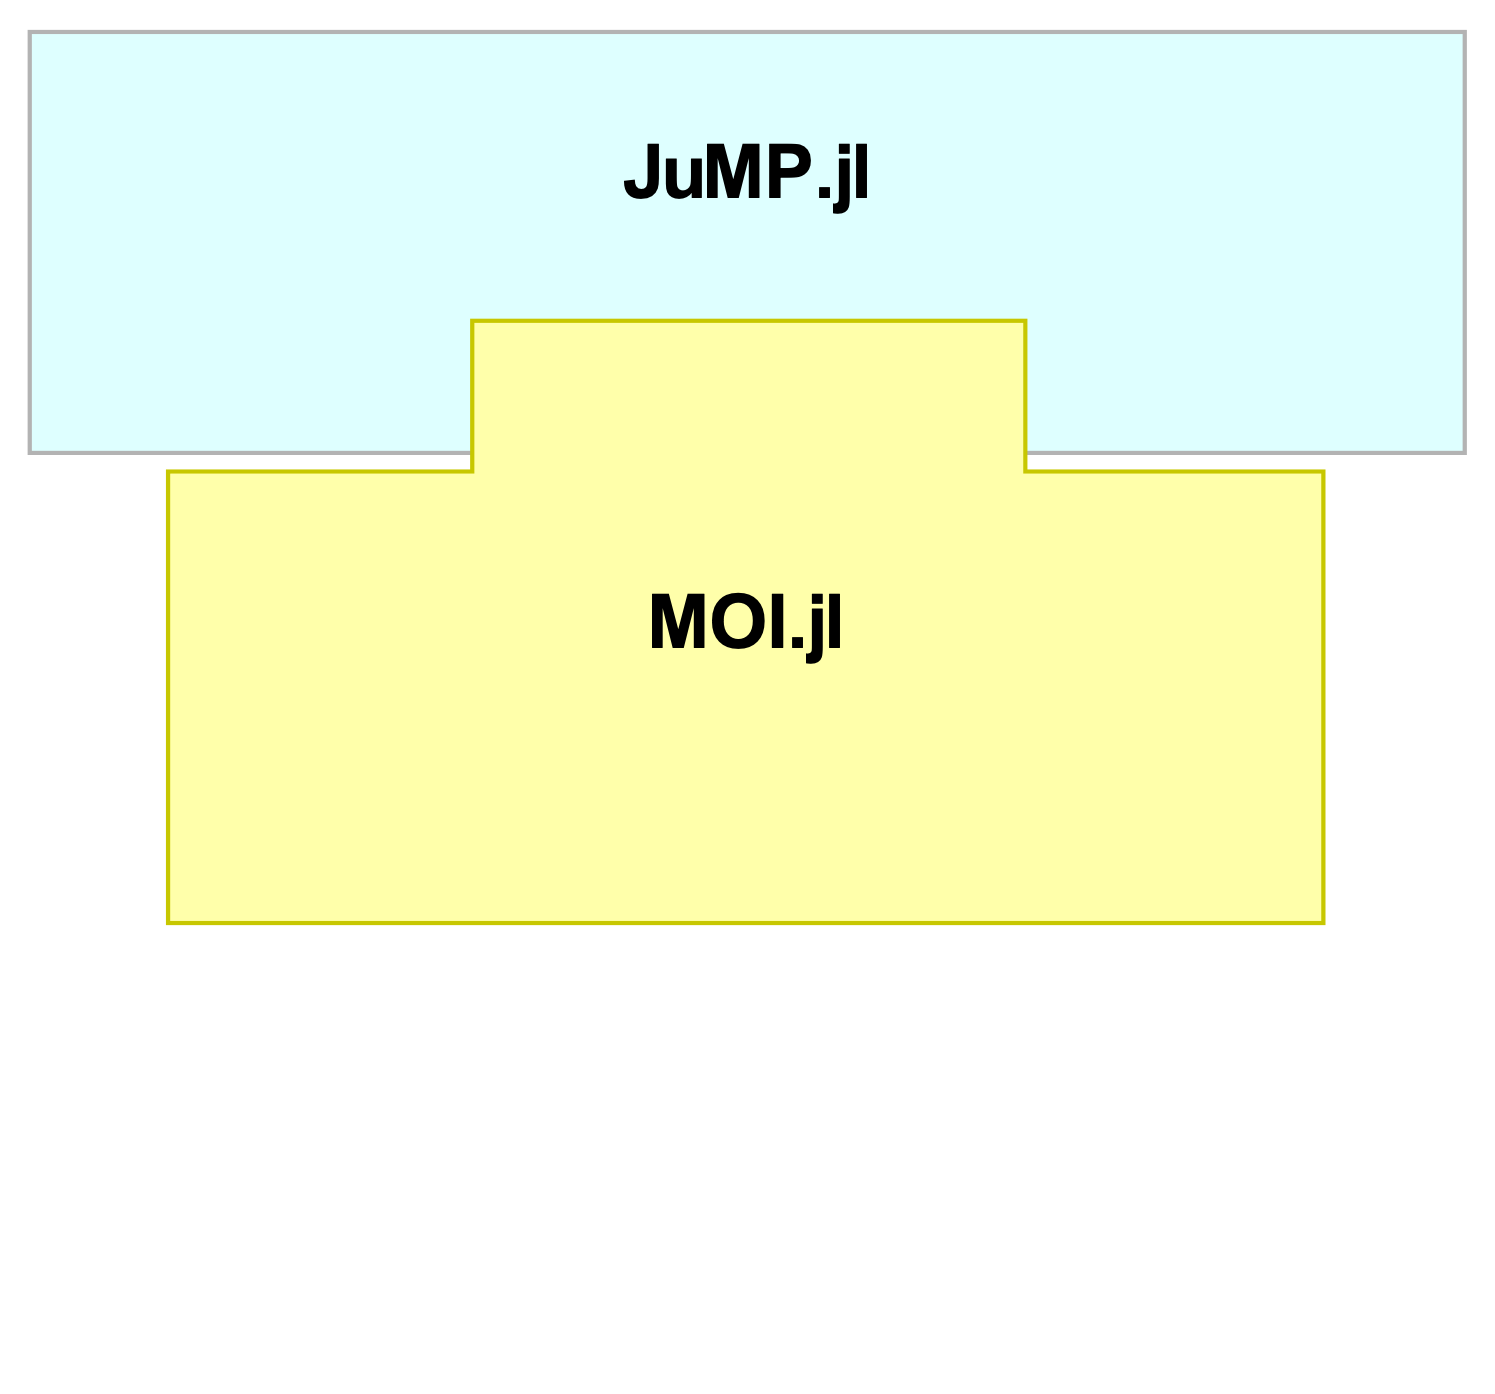
\includegraphics[angle=0,origin=c,height=55mm]{JuMP1.png}}
%\only<2>{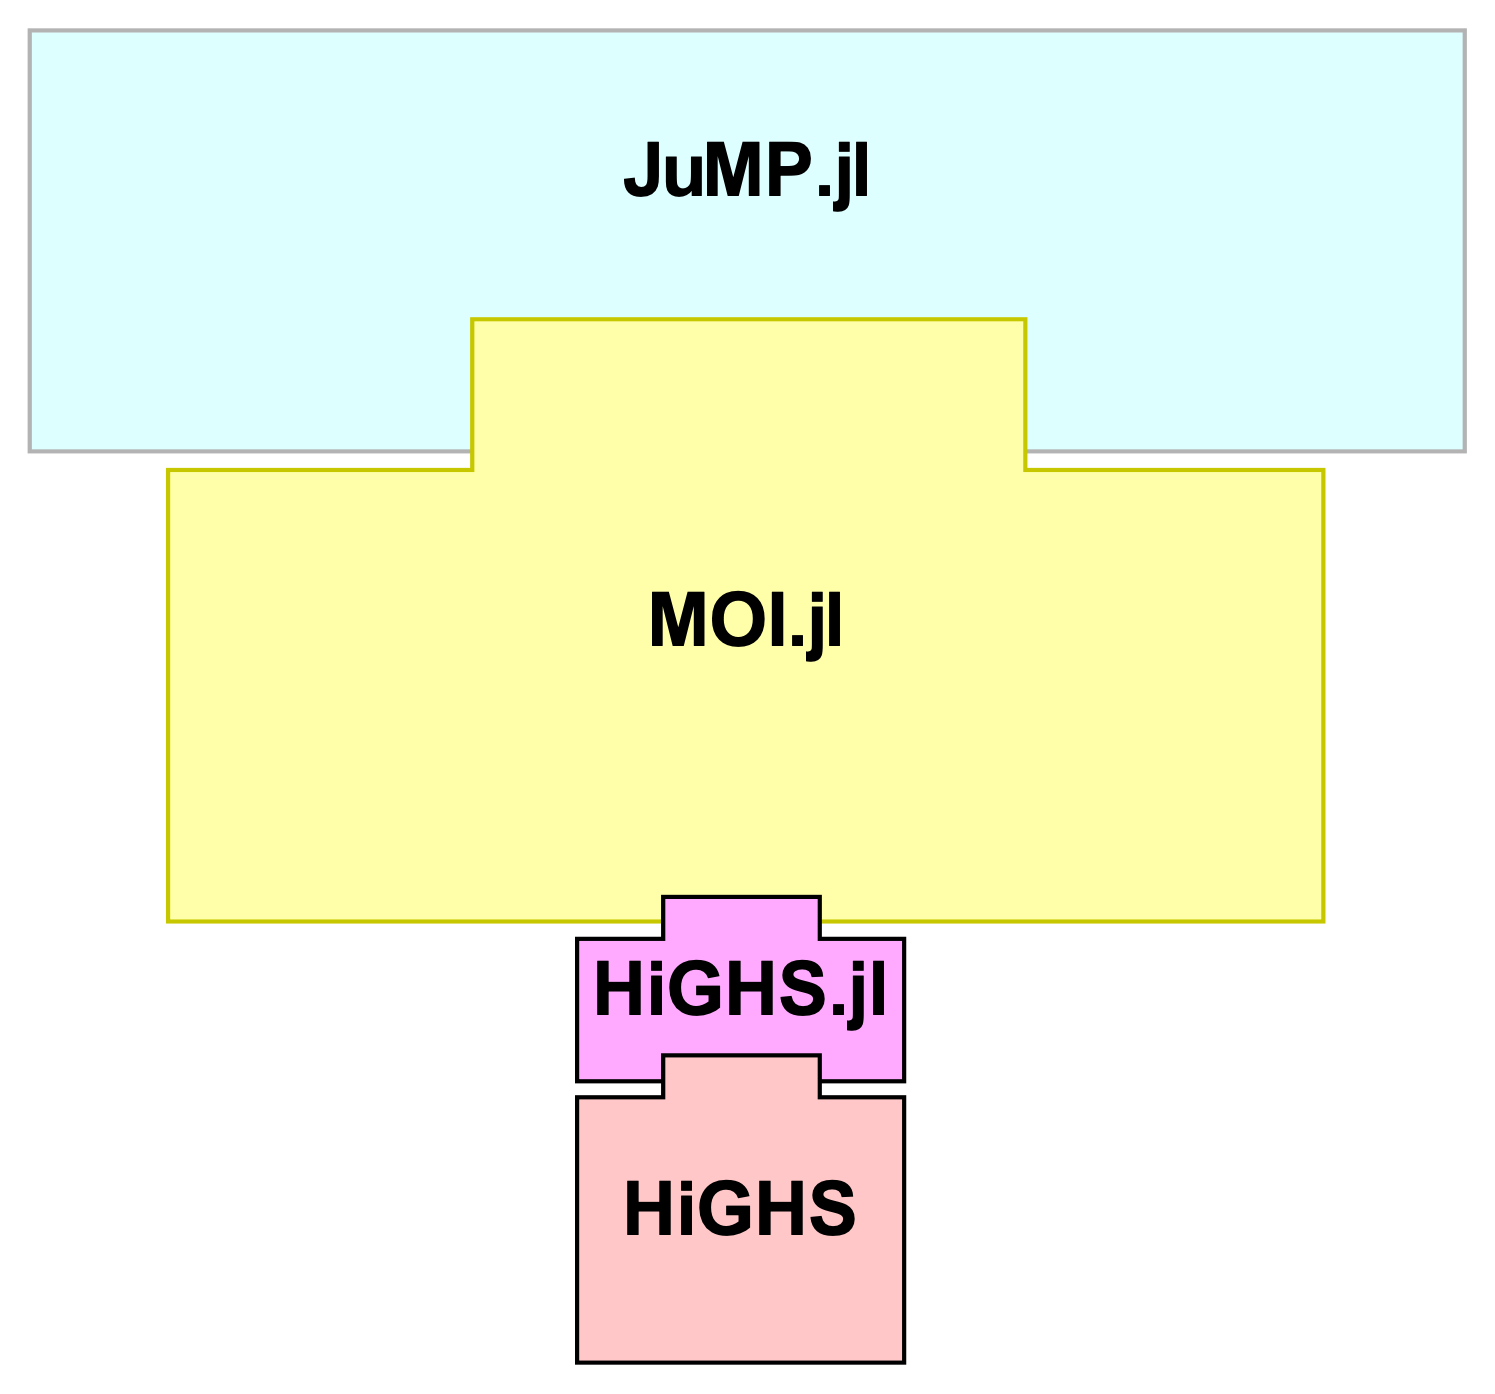
\includegraphics[angle=0,origin=c,height=55mm]{JuMP2.png}}
%\only<2>{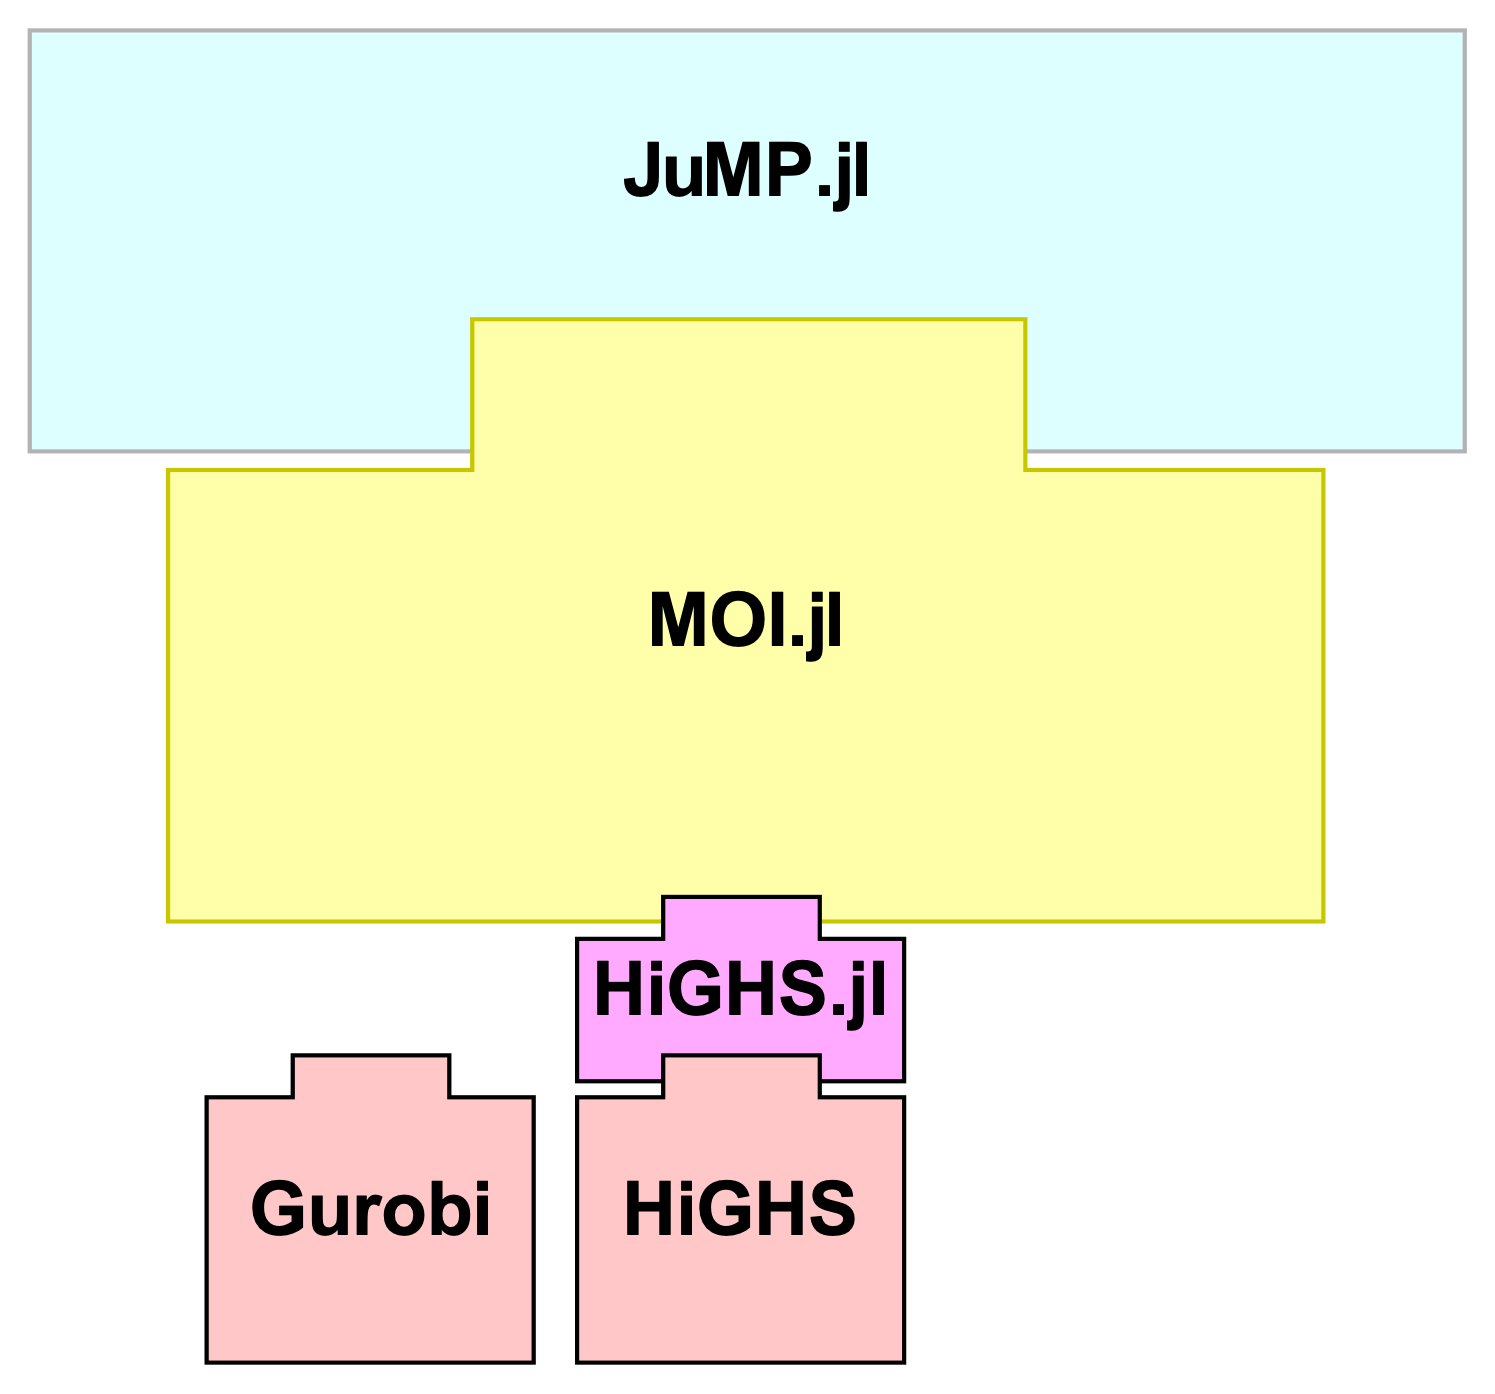
\includegraphics[angle=0,origin=c,height=55mm]{JuMP3.png}}
%\only<3>{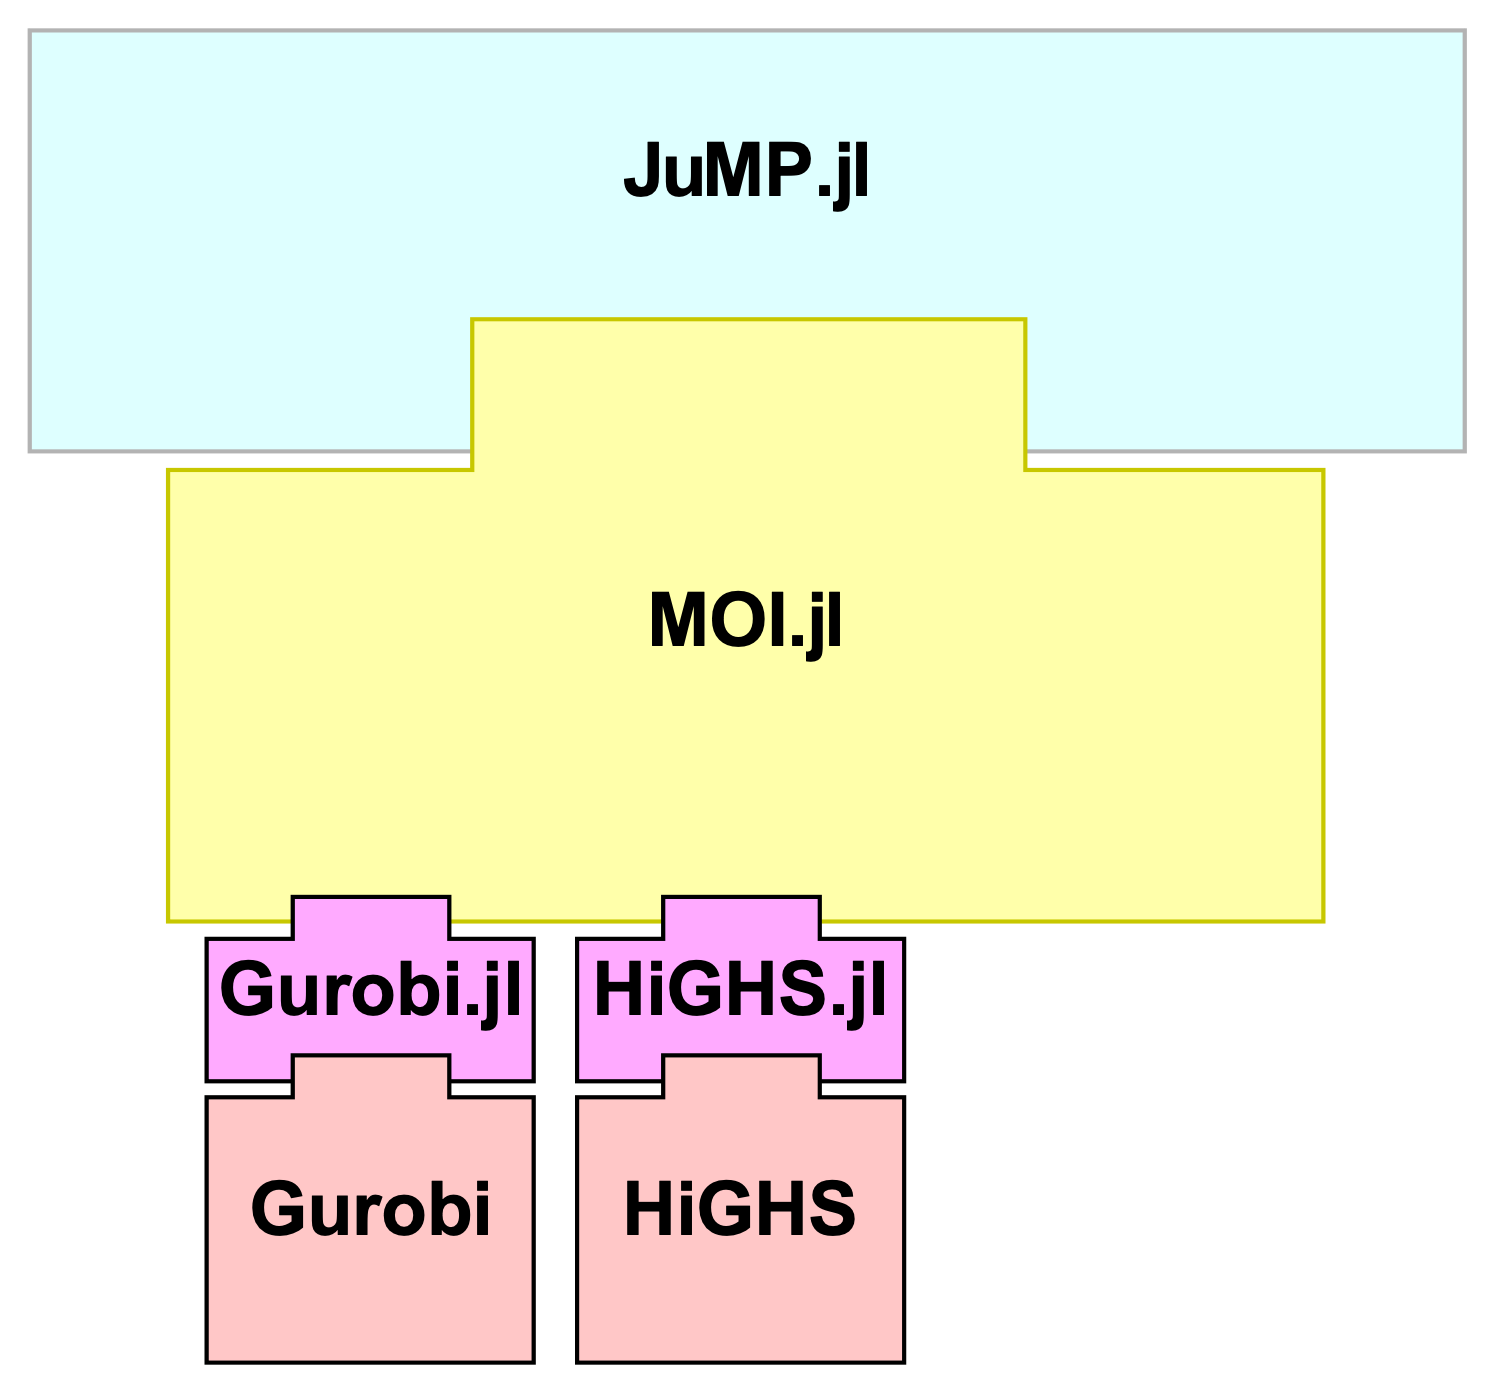
\includegraphics[angle=0,origin=c,height=55mm]{JuMP4.png}}
\only<1>{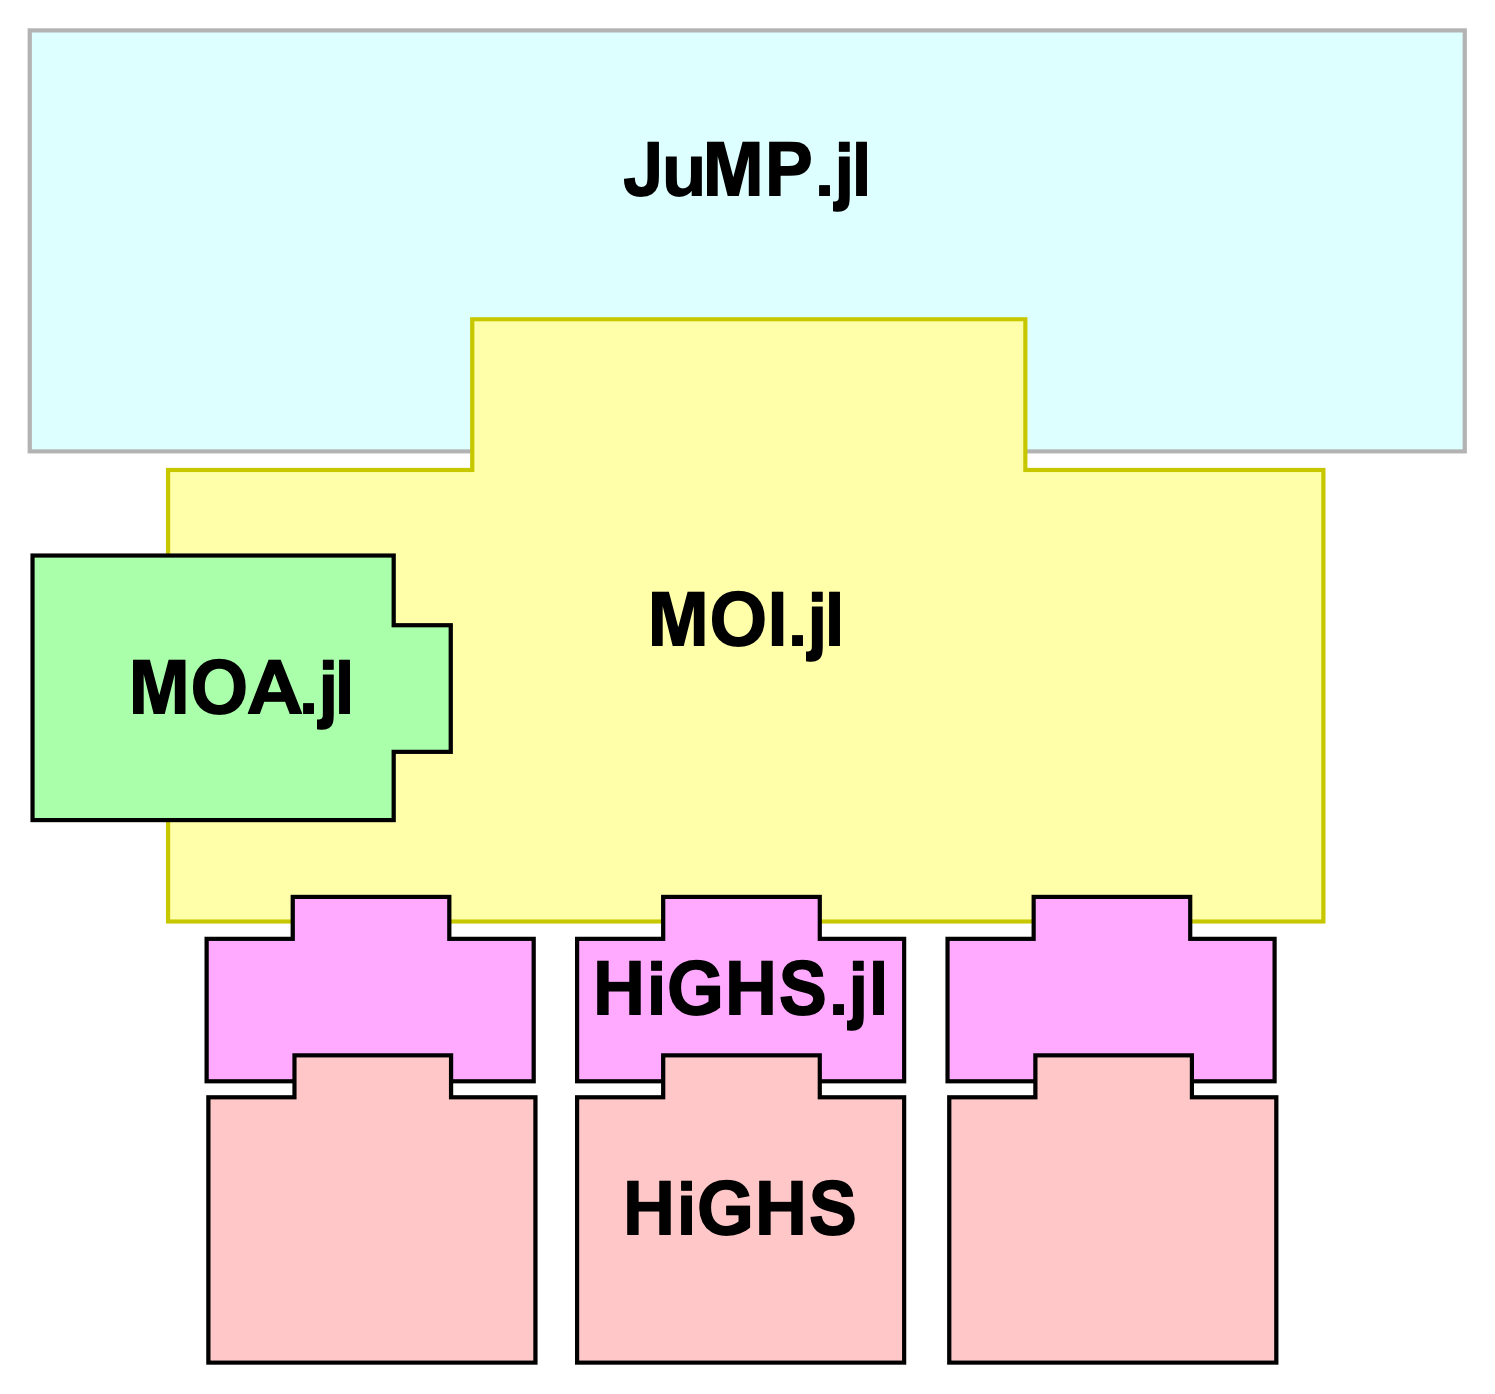
\includegraphics[angle=0,origin=c,height=55mm]{JuMP5.png}}
\end{center}

\end{frame}

% 
% -------------------------------------------------------------------------------------------------------------------------------------------------------
%

\begin{frame}
  \frametitle{Algorithms currently available (v1.3.3)}


\begin{enumerate}
\item     MOA.Lexicographic() [default]  \hfill $p \ge 2$
\item     MOA.Dichotomy()   \hfill $p=2$
\item     MOA.EpsilonConstraint() \hfill $p=2$

%\pause
\medskip

\item     MOA.Hierarchical() \hfill $p \ge 2$
\item     MOA.Chalmet() \hfill $p=2$

\pause
\medskip

\item     MOA.KirlikSayin() \hfill $p \ge 3$
\item     MOA.DominguezRios() \hfill $p \ge 3$
\item     MOA.TambyVanderpooten() \hfill $p \ge 3$
\end{enumerate}
\vspace{6mm}
\pause

\noindent
{+ optimization attributes coming with a given algorithm}

\end{frame}

% 
% -------------------------------------------------------------------------------------------------------------------------------------------------------
%

\begin{frame}
  \frametitle{Zoom on the $\epsilon$-constraint algorithm}
  \medskip

Algorithm:
\begin{itemize}
\item    \blue{\texttt{EpsilonConstraint()}}

\smallskip
\begin{itemize}
\item  []
   {\tiny 
  Y.V. Haimes, L.S. Lasdon, D.A. Wismer (1971). On a bicriterion formation of the problems of integrated system identification and system optimization. \textit{IEEE Transactions on Systems, Man and Cybernetics}, Volume SMC-1, Issue 3, Pages 296-297.\\
  }
 \end{itemize}   
\vspace{-1mm}

  % {\scriptsize for bi-objective programs.}
\end{itemize}   
   

  \bigskip

Attributes:

\begin{itemize}
\item  \blue{\texttt{MOA.EpsilonConstraintStep()}} \\
\smallskip
{\scriptsize 
algorithm uses this value
   as the $\epsilon$ by which it partitions the first-objective's space. The
   default is \texttt{1}, so that for a pure integer program this algorithm will
   enumerate $Y_N$.\\
   }
   \medskip

\item \blue{\texttt{MOA.SolutionLimit()}} \\
\smallskip
{\scriptsize 
if this attribute is set then, instead of using the
   \texttt{MOA.EpsilonConstraintStep}, with a slight abuse of notation,
    \texttt{EpsilonConstraint} divides the range of the first-objective's domain in
   objective space by  \texttt{SolutionLimit} to obtain the  $\epsilon$  to use when
   iterating. Thus, at most  \texttt{SolutionLimit} solutions are returned.\\
   }
\end{itemize}   
\vfill
   
   \end{frame}

%% 
%% -------------------------------------------------------------------------------------------------------------------------------------------------------
%%
%
%\begin{frame}
%  \frametitle{Example (1/5)}
%\vspace{3mm}
%
%\textbf{Compute $X_E$ and $Y_N$ for the following MOP}:
%\vspace{2mm}
%
%    \[
%\begin{array}{crrcrrrl}
%\max z_1 & = & x_1 & + & x_2  \\
%\min z_2 & = & x_1 & + & 3x_2 \vspace{2mm}\\
%s.t. & & 2x_1 & + &  3x_2 & \le & 30 \\
%    &&  3x_1 & + &  2x_2 & \le & 30 \\
%    &&   x_1 & - &   x_2 & \le & 5.5 \vspace{2mm}\\
%    &&   x_1 & , &   x_2 & \in & \mathbb{N}
%\end{array}
%\]
%\vspace{0mm}
%
%\vfill
%
%\end{frame}


% 
% -------------------------------------------------------------------------------------------------------------------------------------------------------
%

\begin{frame}
  \frametitle{Example (1/4)}
%\vspace{3mm}

\hspace{-5mm} \textbf{Compute $X_E$ and $Y_N$ for the following MOP}:
%\vspace{-2mm}

      {\scriptsize
%    \begin{columns}
%      \begin{column}{0.5\textwidth}
    \[
\begin{array}{crrcrrrl}
\max z_1 & = & x_1 & + & x_2  \\
\min z_2 & = & x_1 & + & 3x_2 \vspace{1mm}\\
s.t. & & 2x_1 & + &  3x_2 & \le & 30 \\
    &&  3x_1 & + &  2x_2 & \le & 30 \\
    &&   x_1 & - &   x_2 & \le & 5.5 \vspace{1mm}\\
    &&   x_1 & , &   x_2 & \in & \mathbb{N}
\end{array}
\]

   %   \end{column}
   %   \begin{column}{0.5\textwidth}


%\begin{tcolorbox}[arc=1ex, colback=black!20, colframe=black!20, left=3pt, right=3pt, top=3pt, bottom=2pt]
%%\texttt{ \hspace{-2mm}\green{julia>}  using JuMP, HiGHS}\\
%\texttt{ \hspace{-1.5mm}\green{julia>}  c1 = [1,1]}\\
%\texttt{ \hspace{-2mm}\green{julia>}  c2 = [1,3]}\\
%\texttt{ \hspace{-2mm}\green{julia>}  A  = [2 3; 3 2; 1 -1]} \\
%\texttt{ \hspace{-2mm}\green{julia>}  b  = [30, 30, 5.5]}
%\end{tcolorbox} 
   %   \end{column}
   %   \end{columns} 
}      

\vspace{2mm}


    \begin{columns}
      \begin{column}{0.5\textwidth}
      Decision space:
      
      \begin{center}
      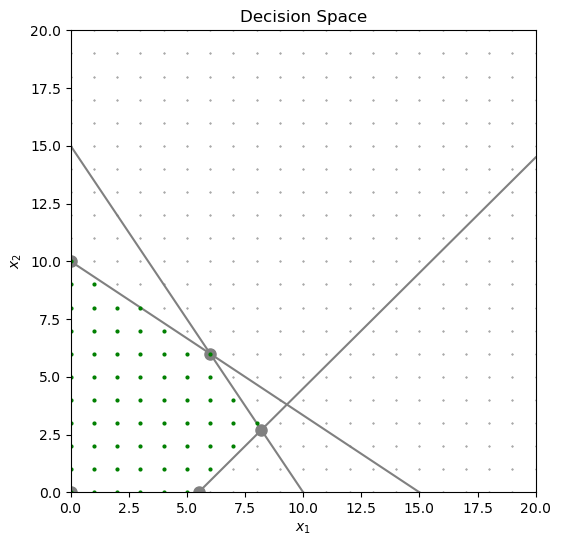
\includegraphics[height=4.25cm]{decisionSpace.png} 
       \end{center}
      \end{column}
      \begin{column}{0.5\textwidth}
      Objective space:
      
      \begin{center}
      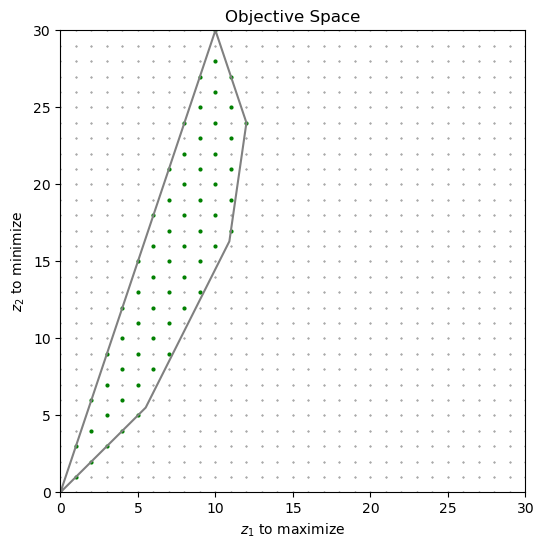
\includegraphics[height=4.25cm]{objectiveSpace.png} 
       \end{center}
      \end{column}
      \end{columns} 

\end{frame}



% 
% -------------------------------------------------------------------------------------------------------------------------------------------------------
%

\begin{frame}
  \frametitle{Example (2/4)}
\vspace{3mm}


%\hspace{-2mm}
Coding the MOO problem with \texttt{JuMP}

{\scriptsize
\begin{tcolorbox}[arc=1ex, colback=black!20, colframe=black!20, left=3pt, right=3pt, top=3pt, bottom=2pt]
\texttt{ \hspace{-1.5mm}\green{julia>}  using JuMP, HiGHS}\\
\texttt{ \hspace{-2mm}\green{julia>}  import MultiObjectiveAlgorithms as MOA}
\end{tcolorbox} 


\begin{tcolorbox}[arc=1ex, colback=black!20, colframe=black!20, left=3pt, right=3pt, top=3pt, bottom=2pt]
\texttt{ \hspace{-1.5mm}\green{julia>} model = Model( ) }\\
\texttt{ \hspace{-2mm}\green{julia>} @variable(model, x1$\ge$0, Int)}\\
\texttt{ \hspace{-2mm}\green{julia>}  @variable(model, x2$\ge$0, Int)}\\
\texttt{ \hspace{-2mm}\green{julia>}  @expression(model, fct1, x1 + x2)     \hfill  \# to maximize}\\
\texttt{ \hspace{-2mm}\green{julia>}  @expression(model, fct2, x1 + 3 * x2)  \hfill \# to minimize}\\
\texttt{ \hspace{-2mm}\green{julia>}  @objective(model, Max,  \redxg{ [fct1, (-1) * fct2]})}\\
\texttt{ \hspace{-2mm}\green{julia>}  @constraint(model, 2*x1 + 3*x2 $\le$ 30)}\\
\texttt{ \hspace{-2mm}\green{julia>}  @constraint(model, 3*x1 + 2*x2 $\le$ 30)}\\
\texttt{ \hspace{-2mm}\green{julia>}  @constraint(model,   x1 -   x2 $\le$ 5.5)}
%\texttt{ \hspace{-2mm}\green{julia>}  }
\end{tcolorbox} 

%\begin{tcolorbox}[arc=1ex, colback=black!20, colframe=black!20, left=3pt, right=3pt, top=3pt, bottom=2pt]
%\texttt{ \hspace{-1.5mm}\green{julia>}   print(model)}
%\end{tcolorbox} 
}


\end{frame}

% 
% -------------------------------------------------------------------------------------------------------------------------------------------------------
%

\begin{frame}
  \frametitle{Example (3/4)}
\vspace{3mm}


Setup the MIP solver: e.g. \texttt{HiGHS}

{\scriptsize
\begin{tcolorbox}[arc=1ex, colback=black!20, colframe=black!20, left=3pt, right=3pt, top=3pt, bottom=2pt]
\texttt{ \hspace{-1.5mm}\green{julia>} set\_optimizer(model,()->\redxg{MOA.Optimizer(HiGHS.Optimizer)})} 
\end{tcolorbox} 
}
\bigskip
\pause

Setup the algorithm: $\epsilon$-constraint; step=1 (default value)

{\scriptsize
\begin{tcolorbox}[arc=1ex, colback=black!20, colframe=black!20, left=3pt, right=3pt, top=3pt, bottom=2pt]
\texttt{ \hspace{-1.5mm}\green{julia>} set\_attribute(model, \redxg{MOA.Algorithm(), MOA.EpsilonConstraint()}) }
\end{tcolorbox} 
}
\bigskip
\pause

Optimize the MOO problem

{\scriptsize
\begin{tcolorbox}[arc=1ex, colback=black!20, colframe=black!20, left=3pt, right=3pt, top=3pt, bottom=2pt]
\texttt{ \hspace{-1.5mm}\green{julia>}  optimize!(model) }
\end{tcolorbox} 
}

\end{frame}

% 
% -------------------------------------------------------------------------------------------------------------------------------------------------------
%

\begin{frame}
  \frametitle{Example  (4/4)}
\vspace{3mm}


Get $X_E$ and $Y_N$

{\scriptsize
\begin{tcolorbox}[arc=1ex, colback=black!20, colframe=black!20, left=3pt, right=3pt, top=3pt, bottom=2pt]
\texttt{ \hspace{-1.5mm}\green{julia>}  for i in 1:\redxg{result\_count(model)} }\\
\texttt{ \hspace{-2mm}\green{julia>}      \qquad z1\_opt = objective\_value(model; \redxg{result = i})\redxg{[1]}}\\
\texttt{ \hspace{-2mm}\green{julia>}      \qquad z2\_opt = -1 * objective\_value(model; \redxg{result = i})\redxg{[2]} }\\
\texttt{ \hspace{-2mm}\green{julia>}      \qquad x1\_opt = value(x1; \redxg{result = i})}\\
\texttt{ \hspace{-2mm}\green{julia>}      \qquad x2\_opt = value(x2; \redxg{result = i}) }\\
\texttt{ \hspace{-2mm}\green{julia>}  end }
\end{tcolorbox} 
}

\vspace{0mm}


    \begin{columns}
      \begin{column}{0.5\textwidth}
      
      \begin{center}
      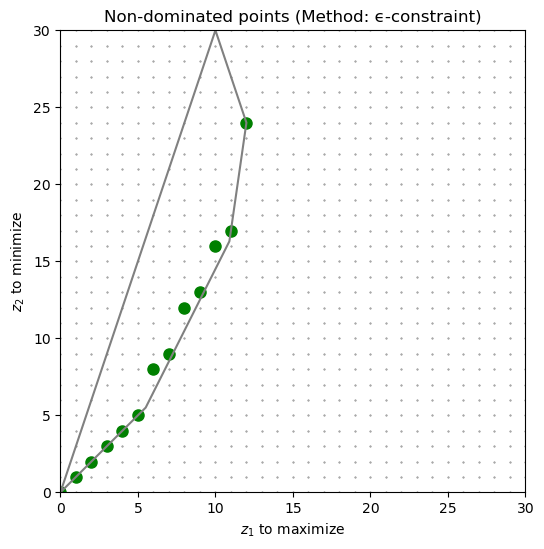
\includegraphics[height=4.25cm]{ndPoints.png} 
       \end{center}
      \end{column}
      \begin{column}{0.5\textwidth}
      
      \begin{center}
      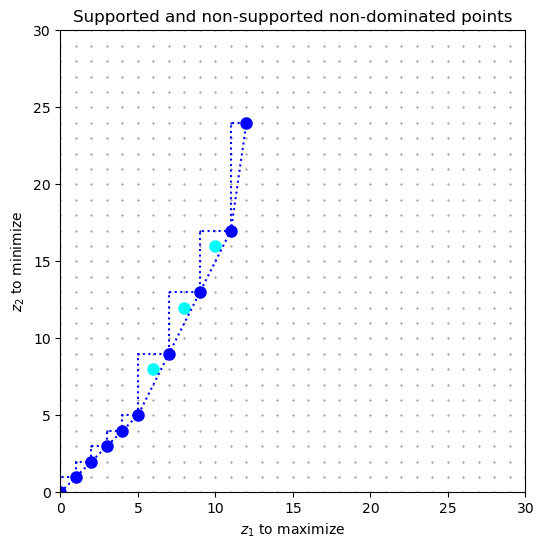
\includegraphics[height=4.25cm]{seNe.png} 
       \end{center}
      \end{column}
      \end{columns} 

\end{frame}

% ================================================================
% ================================================================
% ================================================================


% 
% -------------------------------------------------------------------------------------------------------------------------------------------------------
%
\begin{frame}

\begin{center} 
\Large{From \\ an explicit to an implicit model \\ with JuMP}
\end{center}
              
\end{frame}

% 
% -------------------------------------------------------------------------------------------------------------------------------------------------------
%

\begin{frame}
  \frametitle{Example (1/2)}
%\vspace{3mm}

      {\scriptsize
    \begin{columns}
\hspace{-10mm}        \begin{column}{0.4\textwidth}
  \[
\begin{array}{crrcrrrl}
\max z_1 & = & x_1 & + & x_2  \\
\min z_2 & = & x_1 & + & 3x_2 \vspace{2mm}\\
s.t. & & 2x_1 & + &  3x_2 & \le & \redxg{30} \\
    &&  3x_1 & + &  2x_2 & \le & \redxg{30} \\
    &&   x_1 & - &   x_2 & \le & \redxg{5.5} \vspace{2mm}\\
    &&   x_1 & , &   x_2 & \in & \mathbb{N}
\end{array}
\]
      \end{column}
      %
      %
      \begin{column}{0.5\textwidth} 
    \[
     \  \rightarrow  \quad
\begin{array}{crrcll}
 \max  z_k  = & {\sum_{j=1}^{n} c^k_j x_j}    & & & k=1, \dots , p  \vspace{1mm}\\
 %\min  z_2  = & {\sum_{j=1}^{n} c^2_j x_j}    & & & \vspace{1mm}\\
  s.t &          {\sum_{j=1}^{n} a_{ij} x_j}  &\le&  \redxg{b_i} & i=1, \dots , m   \vspace{1mm}\\
    &         x_j &\in&  \mathbb{N} &  j=1, \dots , n 
\end{array}
\]
\vspace{7mm}
      \end{column}
      \end{columns} 
}      

\vspace{3mm}

{\scriptsize
\begin{tcolorbox}[arc=1ex, colback=black!20, colframe=black!20, left=3pt, right=3pt, top=3pt, bottom=2pt]
%\texttt{ \hspace{-2mm}\green{julia>}  using JuMP, HiGHS}\\
\texttt{ \hspace{-1.5mm}\green{julia>}  c1 = [1,1]; c2 = -1 * [1,3];  c = vcat(c1',c2')}\\
\texttt{ \hspace{-2mm}\green{julia>}  a  = [2 3; 3 2; 1 -1]} \\
\texttt{ \hspace{-2mm}\green{julia>}  \redxg{b  = [30, 30, 5.5]}}\\
\texttt{ \hspace{-2mm}\green{julia>}  m,n = size(a)}\\
\texttt{ \hspace{-2mm}\green{julia>}  p = size(c,1)}
\end{tcolorbox} 

\begin{tcolorbox}[arc=1ex, colback=black!20, colframe=black!20, left=3pt, right=3pt, top=3pt, bottom=2pt]
\texttt{ \hspace{-1.5mm}\green{julia>} md = Model( ) }\\
%
\texttt{ \hspace{-2mm}\textcolor{lightgray}{julia>  @variable(md, x[1:n]$\ge$0, Int)}}\\
%
\texttt{ \hspace{-2mm}\textcolor{lightgray}{julia>  @expression(md, z[k=1:p], sum(c[k,j]*x[j] for j=1:n))}} \\
%\texttt{ \hspace{-2mm}\green{julia>}  @expression(md, z1,  \redxg{sum(c1[j]*x[j] for j=1:n)})  \hfill  \# to maximize}\\
%\texttt{ \hspace{-2mm}\green{julia>}  @expression(md, z2,  \redxg{sum(c2[j]*x[j] for j=1:n)})  \hfill \# to minimize}\\
\texttt{ \hspace{-2mm}\textcolor{lightgray}{julia>  @objective(md, Max, [z[k] for k=1:p])}}\\
%\texttt{ \hspace{-2mm}\green{julia>}  @objective(md, Max,   [z1, (-1) * z2])}\\
%
\texttt{ \hspace{-2mm}\textcolor{lightgray}{julia>   @constraint(md,  ct[i=1:m],  sum(a[i,j]*x[j] for j=1:n) $\le$ b[i])}}
\end{tcolorbox} 
}

\end{frame}


% 
% -------------------------------------------------------------------------------------------------------------------------------------------------------
%

\begin{frame}
  \frametitle{Example (1/2)}
%\vspace{3mm}

      {\scriptsize
    \begin{columns}
\hspace{-10mm}        \begin{column}{0.4\textwidth}
  \[
\begin{array}{crrcrrrl}
\max z_1 & = & x_1 & + & x_2  \\
\min z_2 & = & x_1 & + & 3x_2 \vspace{2mm}\\
s.t. & & 2x_1 & + &  3x_2 & \le & 30 \\
    &&  3x_1 & + &  2x_2 & \le & 30 \\
    &&   x_1 & - &   x_2 & \le & 5.5 \vspace{2mm}\\
    &&   x_1 & , &   x_2 & \in & \mathbb{N}
\end{array}
\]
      \end{column}
      %
      %
      \begin{column}{0.5\textwidth} 
    \[
     \  \rightarrow  \quad
\begin{array}{crrcll}
 \max  z_k  = & {\sum_{j=1}^{n} c^k_j x_j}    & & & k=1, \dots , p  \vspace{1mm}\\
 %\min  z_2  = & {\sum_{j=1}^{n} c^2_j x_j}    & & & \vspace{1mm}\\
  s.t &          {\sum_{j=1}^{n} a_{ij} x_j}  &\le&  b_i & i=1, \dots , m   \vspace{1mm}\\
    &         \redxg{x_j} &\in&  \mathbb{N} & \redxg{ j=1, \dots , n }
\end{array}
\]
\vspace{7mm}
      \end{column}
      \end{columns} 
}      

\vspace{3mm}

{\scriptsize
\begin{tcolorbox}[arc=1ex, colback=black!20, colframe=black!20, left=3pt, right=3pt, top=3pt, bottom=2pt]
%\texttt{ \hspace{-2mm}\green{julia>}  using JuMP, HiGHS}\\
\texttt{ \hspace{-1.5mm}\green{julia>}  c1 = [1,1]; c2 = -1 * [1,3];  c = vcat(c1',c2')}\\
\texttt{ \hspace{-2mm}\green{julia>}  a  = [2 3; 3 2; 1 -1]} \\
\texttt{ \hspace{-2mm}\green{julia>}  b  = [30, 30, 5.5]}\\
\texttt{ \hspace{-2mm}\green{julia>}  m,n = size(a)}\\
\texttt{ \hspace{-2mm}\green{julia>}  p = size(c,1)}
\end{tcolorbox} 

\begin{tcolorbox}[arc=1ex, colback=black!20, colframe=black!20, left=3pt, right=3pt, top=3pt, bottom=2pt]
\texttt{ \hspace{-1.5mm}\green{julia>} md = Model( ) }\\
%
\texttt{ \hspace{-2mm}\green{julia>}  @variable(md, \redxg{x[1:n]}$\ge$0, Int)}\\
%
\texttt{ \hspace{-2mm}\textcolor{lightgray}{julia>  @expression(md, z[k=1:p], sum(c[k,j]*x[j] for j=1:n))}} \\
%\texttt{ \hspace{-2mm}\green{julia>}  @expression(md, z1,  \redxg{sum(c1[j]*x[j] for j=1:n)})  \hfill  \# to maximize}\\
%\texttt{ \hspace{-2mm}\green{julia>}  @expression(md, z2,  \redxg{sum(c2[j]*x[j] for j=1:n)})  \hfill \# to minimize}\\
\texttt{ \hspace{-2mm}\textcolor{lightgray}{julia>  @objective(md, Max, [z[k] for k=1:p])}}\\
%\texttt{ \hspace{-2mm}\green{julia>}  @objective(md, Max,   [z1, (-1) * z2])}\\
%
\texttt{ \hspace{-2mm}\textcolor{lightgray}{julia>   @constraint(md,  ct[i=1:m],  sum(a[i,j]*x[j] for j=1:n) $\le$ b[i])}}
\end{tcolorbox} 
}

\end{frame}


% 
% -------------------------------------------------------------------------------------------------------------------------------------------------------
%

\begin{frame}
  \frametitle{Example (1/2)}
%\vspace{3mm}

      {\scriptsize
    \begin{columns}
\hspace{-10mm}        \begin{column}{0.4\textwidth}
  \[
\begin{array}{crrcrrrl}
\max z_1 & = & x_1 & + & x_2  \\
\min z_2 & = & x_1 & + & 3x_2 \vspace{2mm}\\
s.t. & & 2x_1 & + &  3x_2 & \le & 30 \\
    &&  3x_1 & + &  2x_2 & \le & 30 \\
    &&   x_1 & - &   x_2 & \le & 5.5 \vspace{2mm}\\
    &&   x_1 & , &   x_2 & \in & \mathbb{N}
\end{array}
\]
      \end{column}
      %
      %
      \begin{column}{0.5\textwidth} 
    \[
     \  \rightarrow  \quad
\begin{array}{crrcll}
 \max  z_k  = & \redxg{{\sum_{j=1}^{n} c^k_j x_j}}    & & & \redxg{k=1, \dots , p}  \vspace{1mm}\\
 %\min  z_2  = & {\sum_{j=1}^{n} c^2_j x_j}    & & & \vspace{1mm}\\
  s.t &          {\sum_{j=1}^{n} a_{ij} x_j}  &\le&  b_i & i=1, \dots , m   \vspace{1mm}\\
    &         x_j &\in&  \mathbb{N}  &  j=1, \dots , n 
\end{array}
\]
\vspace{7mm}
      \end{column}
      \end{columns} 
}      

\vspace{3mm}

{\scriptsize
\begin{tcolorbox}[arc=1ex, colback=black!20, colframe=black!20, left=3pt, right=3pt, top=3pt, bottom=2pt]
%\texttt{ \hspace{-2mm}\green{julia>}  using JuMP, HiGHS}\\
\texttt{ \hspace{-1.5mm}\green{julia>}  c1 = [1,1]; c2 = -1 * [1,3];  c = vcat(c1',c2')}\\
\texttt{ \hspace{-2mm}\green{julia>}  a  = [2 3; 3 2; 1 -1]} \\
\texttt{ \hspace{-2mm}\green{julia>}  b  = [30, 30, 5.5]}\\
\texttt{ \hspace{-2mm}\green{julia>}  m,n = size(a)}\\
\texttt{ \hspace{-2mm}\green{julia>}  p = size(c,1)}
\end{tcolorbox} 

\begin{tcolorbox}[arc=1ex, colback=black!20, colframe=black!20, left=3pt, right=3pt, top=3pt, bottom=2pt]
\texttt{ \hspace{-1.5mm}\green{julia>} md = Model( ) }\\
%
\texttt{ \hspace{-2mm}\green{julia>}  @variable(md, \redxg{x[1:n]}$\ge$0, Int)}\\
%
\texttt{ \hspace{-2mm}\green{julia>}  @expression(md, \redxg{z[k=1:p], sum(c[k,j]*x[j] for j=1:n)})} \\
%\texttt{ \hspace{-2mm}\green{julia>}  @expression(md, z1,  \redxg{sum(c1[j]*x[j] for j=1:n)})  \hfill  \# to maximize}\\
%\texttt{ \hspace{-2mm}\green{julia>}  @expression(md, z2,  \redxg{sum(c2[j]*x[j] for j=1:n)})  \hfill \# to minimize}\\
\texttt{ \hspace{-2mm}\textcolor{lightgray}{julia>  @objective(md, Max, [z[k] for k=1:p])}}\\
%\texttt{ \hspace{-2mm}\green{julia>}  @objective(md, Max,   [z1, (-1) * z2])}\\
%
\texttt{ \hspace{-2mm}\textcolor{lightgray}{julia>   @constraint(md,  ct[i=1:m],  sum(a[i,j]*x[j] for j=1:n) $\le$ b[i])}}
\end{tcolorbox} 
}

\end{frame}

% 
% -------------------------------------------------------------------------------------------------------------------------------------------------------
%

\begin{frame}
  \frametitle{Example (1/2)}
%\vspace{3mm}

      {\scriptsize
    \begin{columns}
\hspace{-10mm}        \begin{column}{0.4\textwidth}
  \[
\begin{array}{crrcrrrl}
\max z_1 & = & x_1 & + & x_2  \\
\min z_2 & = & x_1 & + & 3x_2 \vspace{2mm}\\
s.t. & & 2x_1 & + &  3x_2 & \le & 30 \\
    &&  3x_1 & + &  2x_2 & \le & 30 \\
    &&   x_1 & - &   x_2 & \le & 5.5 \vspace{2mm}\\
    &&   x_1 & , &   x_2 & \in & \mathbb{N}
\end{array}
\]
      \end{column}
      %
      %
      \begin{column}{0.5\textwidth} 
    \[
     \  \rightarrow  \quad
\begin{array}{crrcll}
 \max  \redxg{z_k}  = & {\sum_{j=1}^{n} c^k_j x_j}    & & & \redxg{k=1, \dots , p}  \vspace{1mm}\\
 %\min  z_2  = & {\sum_{j=1}^{n} c^2_j x_j}    & & & \vspace{1mm}\\
  s.t &          {\sum_{j=1}^{n} a_{ij} x_j}  &\le&  b_i & i=1, \dots , m   \vspace{1mm}\\
    &         x_j &\in&  \mathbb{N}  &  j=1, \dots , n 
\end{array}
\]
\vspace{7mm}
      \end{column}
      \end{columns} 
}      

\vspace{3mm}

{\scriptsize
\begin{tcolorbox}[arc=1ex, colback=black!20, colframe=black!20, left=3pt, right=3pt, top=3pt, bottom=2pt]
%\texttt{ \hspace{-2mm}\green{julia>}  using JuMP, HiGHS}\\
\texttt{ \hspace{-1.5mm}\green{julia>}  c1 = [1,1]; c2 = -1 * [1,3];  c = vcat(c1',c2')}\\
\texttt{ \hspace{-2mm}\green{julia>}  a  = [2 3; 3 2; 1 -1]} \\
\texttt{ \hspace{-2mm}\green{julia>}  b  = [30, 30, 5.5]}\\
\texttt{ \hspace{-2mm}\green{julia>}  m,n = size(a)}\\
\texttt{ \hspace{-2mm}\green{julia>}  p = size(c,1)}
\end{tcolorbox} 

\begin{tcolorbox}[arc=1ex, colback=black!20, colframe=black!20, left=3pt, right=3pt, top=3pt, bottom=2pt]
\texttt{ \hspace{-1.5mm}\green{julia>} md = Model( ) }\\
%
\texttt{ \hspace{-2mm}\green{julia>}  @variable(md, \redxg{x[1:n]}$\ge$0, Int)}\\
%
\texttt{ \hspace{-2mm}\green{julia>}  @expression(md, \redxg{z[k=1:p], sum(c[k,j]*x[j] for j=1:n)})} \\
%\texttt{ \hspace{-2mm}\green{julia>}  @expression(md, z1,  \redxg{sum(c1[j]*x[j] for j=1:n)})  \hfill  \# to maximize}\\
%\texttt{ \hspace{-2mm}\green{julia>}  @expression(md, z2,  \redxg{sum(c2[j]*x[j] for j=1:n)})  \hfill \# to minimize}\\
\texttt{ \hspace{-2mm}\green{julia>}  @objective(md, Max, \redxg{[z[k] for k=1:p]})}\\
%\texttt{ \hspace{-2mm}\green{julia>}  @objective(md, Max,   [z1, (-1) * z2])}\\
%
\texttt{ \hspace{-2mm}\textcolor{lightgray}{julia>   @constraint(md,  ct[i=1:m],  sum(a[i,j]*x[j] for j=1:n) $\le$ b[i])}}
\end{tcolorbox} 
}

\end{frame}


% 
% -------------------------------------------------------------------------------------------------------------------------------------------------------
%

\begin{frame}
  \frametitle{Example (1/2)}
%\vspace{3mm}

      {\scriptsize
    \begin{columns}
\hspace{-10mm}        \begin{column}{0.4\textwidth}
  \[
\begin{array}{crrcrrrl}
\max z_1 & = & x_1 & + & x_2  \\
\min z_2 & = & x_1 & + & 3x_2 \vspace{2mm}\\
s.t. & & 2x_1 & + &  3x_2 & \le & 30 \\
    &&  3x_1 & + &  2x_2 & \le & 30 \\
    &&   x_1 & - &   x_2 & \le & 5.5 \vspace{2mm}\\
    &&   x_1 & , &   x_2 & \in & \mathbb{N}
\end{array}
\]
      \end{column}
      %
      %
      \begin{column}{0.5\textwidth} 
    \[
     \  \rightarrow  \quad
\begin{array}{crrcll}
 \max  z_k  = & {\sum_{j=1}^{n} c^k_j x_j}    & & & k=1, \dots , p  \vspace{1mm}\\
 %\min  z_2  = & {\sum_{j=1}^{n} c^2_j x_j}    & & & \vspace{1mm}\\
  s.t &          \redxg{{\sum_{j=1}^{n} a_{ij} x_j} } &\le&  \redxg{b_i} & \redxg{i=1, \dots , m}   \vspace{1mm}\\
    &         x_j &\in&  \mathbb{N}  &  j=1, \dots , n 
\end{array}
\]
\vspace{7mm}
      \end{column}
      \end{columns} 
}      

\vspace{3mm}

{\scriptsize
\begin{tcolorbox}[arc=1ex, colback=black!20, colframe=black!20, left=3pt, right=3pt, top=3pt, bottom=2pt]
%\texttt{ \hspace{-2mm}\green{julia>}  using JuMP, HiGHS}\\
\texttt{ \hspace{-1.5mm}\green{julia>}  c1 = [1,1]; c2 = -1 * [1,3];  c = vcat(c1',c2')}\\
\texttt{ \hspace{-2mm}\green{julia>}  a  = [2 3; 3 2; 1 -1]} \\
\texttt{ \hspace{-2mm}\green{julia>}  b  = [30, 30, 5.5]}\\
\texttt{ \hspace{-2mm}\green{julia>}  m,n = size(a)}\\
\texttt{ \hspace{-2mm}\green{julia>}  p = size(c,1)}
\end{tcolorbox} 

\begin{tcolorbox}[arc=1ex, colback=black!20, colframe=black!20, left=3pt, right=3pt, top=3pt, bottom=2pt]
\texttt{ \hspace{-1.5mm}\green{julia>} md = Model( ) }\\
%
\texttt{ \hspace{-2mm}\green{julia>}  @variable(md, \redxg{x[1:n]}$\ge$0, Int)}\\
%
\texttt{ \hspace{-2mm}\green{julia>}  @expression(md, \redxg{z[k=1:p], sum(c[k,j]*x[j] for j=1:n)})} \\
%\texttt{ \hspace{-2mm}\green{julia>}  @expression(md, z1,  \redxg{sum(c1[j]*x[j] for j=1:n)})  \hfill  \# to maximize}\\
%\texttt{ \hspace{-2mm}\green{julia>}  @expression(md, z2,  \redxg{sum(c2[j]*x[j] for j=1:n)})  \hfill \# to minimize}\\
\texttt{ \hspace{-2mm}\green{julia>}  @objective(md, Max, \redxg{[z[k] for k=1:p]})}\\
%\texttt{ \hspace{-2mm}\green{julia>}  @objective(md, Max,   [z1, (-1) * z2])}\\
%
\texttt{ \hspace{-2mm}\green{julia>}  @constraint(md,  \redxg{ct[i=1:m]},  \redxg{sum(a[i,j]*x[j] for j=1:n) $\le$ b[i]})}
\end{tcolorbox} 
}

\end{frame}


% 
% -------------------------------------------------------------------------------------------------------------------------------------------------------
%

\begin{frame}
  \frametitle{Example  (2/2)}
\vspace{3mm}


Get $X_E$ and $Y_N$

{\scriptsize
\begin{tcolorbox}[arc=1ex, colback=black!20, colframe=black!20, left=3pt, right=3pt, top=3pt, bottom=2pt]
\texttt{ \hspace{-1.5mm}\green{julia>}  for i in 1:result\_count(model) }\\
%\texttt{ \hspace{-2mm}\green{julia>}      \qquad z1\_opt = objective\_value(model; result = i)[1]}\\
%\texttt{ \hspace{-2mm}\green{julia>}      \qquad z2\_opt = -1 * objective\_value(model; result = i)[2] }\\
\texttt{ \hspace{-2mm}\green{julia>}      \qquad z\_opt = [objective\_value(md; result = i)[k] for k=1:p] }\\
\texttt{ \hspace{-2mm}\green{julia>}      \qquad x\_opt = value\redxg{.}(x; result = i)}\\
\texttt{ \hspace{-2mm}\green{julia>}  end }
\end{tcolorbox} 
}
\vspace{2mm}


Plot $Y_N$
{\scriptsize
\begin{tcolorbox}[arc=1ex, colback=black!20, colframe=black!20, left=3pt, right=3pt, top=3pt, bottom=2pt]
\texttt{ \hspace{-1.5mm}\green{julia>} using Plots }\\
\texttt{ \hspace{-1.5mm}\green{julia>} Plots.scatter( }\\
\texttt{ \hspace{-1.5mm}\green{julia>} \                  [value(z[1]; result = i) for i in 1:result\_count(md)], }\\
\texttt{ \hspace{-1.5mm}\green{julia>} \                  [-1 * value(z[2]; result = i) for i in 1:result\_count(md)]; }\\
\texttt{ \hspace{-1.5mm}\green{julia>} \                  xlabel = "objective 1", }\\
\texttt{ \hspace{-1.5mm}\green{julia>} \                  ylabel = "objective 2", }\\
\texttt{ \hspace{-1.5mm}\green{julia>} \                  title = "objective space", }\\
\texttt{ \hspace{-1.5mm}\green{julia>} \                  legend = false, }\\
\texttt{ \hspace{-1.5mm}\green{julia>} \                  xlims = (0,25), }\\
\texttt{ \hspace{-1.5mm}\green{julia>} \                  ylims = (0,25), }\\
\texttt{ \hspace{-1.5mm}\green{julia>} \                  aspect\_ratio=:equal, }\\
\texttt{ \hspace{-1.5mm}\green{julia>}              ) }
\end{tcolorbox} 
}

\end{frame}

% 
% -------------------------------------------------------------------------------------------------------------------------------------------------------
%

\begin{frame}
  \frametitle{More...}
\vspace{3mm}

{\footnotesize

Oscar Dowson, Xavier Gandibleux, Gokhan Kof. 
From vOptGeneric.jl to MultiObjectiveAlgorithms.jl \ \textit{JuliaDays 2023}, 4-6 October 2023. Paris (France).\vspace{10mm}\\


%\begin{itemize}
  %\item 
    \hspace{0mm}\blue{JuMP}:\\
    \hspace{0mm}{\scriptsize \url{https://jump.dev/}}\\
\vspace{5mm}
  
  %\item 
    \hspace{0mm}\blue{MultiObjectiveAlgorithms}:\\
    \hspace{0mm}{\scriptsize \url{https://github.com/jump-dev/MultiObjectiveAlgorithms.jl}}\\
\vspace{5mm}
  
  %\item 
    \hspace{0mm}\blue{Examples:}\\
    \hspace{0mm}{\scriptsize \url{https://jump.dev/JuMP.jl/stable/tutorials/linear/multi\_objective\_examples/}}\\
%\end{itemize}
\vspace{10mm}
  %\item 
   % \hspace{0mm}\blue{vOptSolver}:\\
   % \hspace{0mm}{\scriptsize \url{https://github.com/vOptSolver}}\\
%\vspace{5mm}

}
\end{frame}

% 
% -------------------------------------------------------------------------------------------------------------------------------------------------------
%

\begin{frame}
  \frametitle{Roadmap}
\vspace{3mm}

The missing parts

\begin{itemize}
\item solving MOLP with a  multi-objective simplex algorithm\\
$\drsh$ working on HiGHS2LP, a parametric variant of HiGHS
\pause
\item solving MOMILP with a  branch-and-xx algorithm\\
$\drsh$ works in progress in the literature 
\pause
\item detecting problem-specific structure in a presolve\\
$\drsh$ solving MOCO with specific algorithms 
\end{itemize}


\end{frame}




% 
% -------------------------------------------------------------------------------------------------------------------------------------------------------
%

\begin{frame}
  \frametitle{Practice}
\vspace{3mm}

\begin{enumerate}
\item Installing the packages MultiObjectiveAlgorithms and Plots

\item Coding and solving a MOIP problem \vspace{3mm}

\end{enumerate}
\end{frame}


% 
% -------------------------------------------------------------------------------------------------------------------------------------------------------
%

\begin{frame}
  \frametitle{Call for participation}
\vspace{3mm}



\hspace{-3mm}
\includegraphics[height=1.95cm]{logoparis.png}     \vspace{2mm}\\
\begin{itemize}
\item[] \small{European conference on the Julia programming language}\vspace{-1mm}
\item[] October 2-3, 2025 --- Paris (France)\vspace{-1mm}\\
\smallskip
\url{https://juliacon.org/}
\end{itemize}    
          

\vspace{6mm}

    \begin{columns}
      \begin{column}{0.575\textwidth}
Keynote Speakers: \vspace{2mm}\\

\begin{itemize}
\item[] Laura Grigori (EPFL, Switzerland)\vspace{-1mm}

\item[] Ivet Galabova (HiGHS, Scotland)\vspace{-1mm}

\item[] Tim Besard (JuliaHub, Belgium)\vspace{-1mm}
\end{itemize}
\vspace{4mm}
      \end{column}
      \begin{column}{0.35\textwidth}
Venue:\vspace{2mm}\\
\begin{itemize}
\item[] 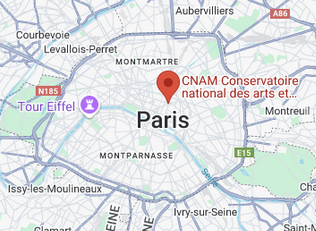
\includegraphics[height=2.0cm]{localisationCNAM.png} 
\end{itemize}
      \end{column}
    \end{columns}






\end{frame}

\end{document}
% 
% -------------------------------------------------------------------------------------------------------------------------------------------------------
%

\begin{frame}
%  \frametitle{Slides suivants...}
  
      \vspace{7mm}
    \centerline{
\includegraphics[height=6cm]{imageMire.png}}
    \vspace{5mm}
    
%  \href{run:./FctOI-1-1-THEME1representations.pdf}{\centerline{\Large{\textcolor{nblue}{Next: Getting started}}}}
  
\end{frame}

  
\end{document}  



    


